%% ====================================================================
%%  Towards Longitudinal Prediction of Parkinson's Disease Motor Subtypes
%%  Preprint source.  pdflatex -> bibtex -> pdflatex x2
%% ====================================================================
\documentclass[11pt]{article}

\usepackage[T1]{fontenc}
\usepackage[utf8]{inputenc}
\usepackage{amsmath,amssymb}
\let\Bbbk\relax
\usepackage{newtxtext,newtxmath}
\usepackage[margin=1.15in]{geometry}
\usepackage{graphicx}
\usepackage{booktabs}
\usepackage{longtable}
\usepackage{array}
\usepackage{authblk}
\usepackage[numbers,sort&compress]{natbib}
\usepackage{microtype}
\usepackage{url}
\usepackage[font=small,labelfont=bf,width=.95\textwidth]{caption}
\usepackage{fancyhdr}
\usepackage[hidelinks]{hyperref}

\graphicspath{{figures/}}

\renewcommand{\arraystretch}{1.08}
\setlength{\parskip}{0pt}
\setlength{\skip\footins}{14pt}
\setlength{\bibsep}{4pt}

\pagestyle{fancy}
\fancyhf{}
\renewcommand{\headrulewidth}{0pt}
\fancyfoot[C]{\thepage}

\newcommand{\TD}{\mathrm{TD}}
\newcommand{\PIGD}{\mathrm{PIGD}}
\newcommand{\Ind}{\mathrm{Ind}}

\title{\bfseries Towards Longitudinal Prediction of\\
Parkinson's Disease Motor Subtypes}

\author[1]{Parv Patel}
\author[1]{Mayank Tewatia}
\author[2]{Varsha Vasudevan}
\author[1]{K.~R.~Sahasranand}
\affil[1]{\normalsize Indian Institute of Technology Palakkad, India}
\affil[2]{\normalsize NeuroComp}

\date{}

\begin{document}
\maketitle
\thispagestyle{fancy}

\begin{abstract}
\noindent
Parkinson's disease is commonly divided into tremor-dominant (TD) and postural
instability and gait difficulty (PIGD) motor subtypes, with an Indeterminate
band between them. The subtype is obtained by thresholding the ratio of two
averages of MDS-UPDRS items, and a change of subtype over time is widely
treated as a marker of motor progression. Much modelling work therefore aims to
predict this label, but the reliability of the label itself is rarely measured
first. We ask whether longitudinal prediction of the motor subtype is limited
by the choice of model family, or by the reliability and representation of the
label being predicted.

We assembled a frozen visit panel from the Parkinson's Progression Markers
Initiative: 1,080 patients and 4,441 labelled visits, of which 934 patients with
two or more labelled visits contribute 3,361 consecutive visit-to-visit
transitions. We first characterised the label without fitting anything. It is
reconstructed exactly from the raw items, but the same visit scored from the
OFF-medication and the ON-medication examination carries the same label at only
75.2\% of pairs; the ratio lives on an integer lattice on which the
Indeterminate band of width 0.25 admits just eleven attainable values, 78\% of
them within 0.02 of a threshold; and moving both thresholds by less than that
spacing relabels 6.7\% of all labelled visits and a fifth of patients, every one
of them out of the Indeterminate class. Over the transitions, 35.2\% of observed
subtype changes revert at the very next visit, requiring a conversion to hold
for two consecutive assessments removes 51.7\% of apparent PIGD conversions
(263 to 127), and the recorded label fails a first-order Markov test in all
three current states ($P \leq 0.004$).

We then fitted and compared model families spanning discrete-time and
continuous-time Markov chains on the observed label; a hidden Markov model with
a latent state and a fitted misclassification matrix; a hierarchical Bayesian
growth model of the ratio and its Student-t variants; Gaussian process
regression on the ratio and on the tremor and PIGD subscores; joint and
multi-output subscore models; time-varying spline mixed models; a discrete
latent clinical state over ten measurements; a continuous nine-domain
level-and-rate profile; and a latent-state model whose observation alphabet
carries the ratio band. Evaluation is leave-one-patient-out with
patient-clustered bootstrap intervals, and all fourteen three-class
specifications are scored on one common case list under one decision rule.

A pre-registered posterior-predictive check rejects the natural continuous
generative model of the label ($T_{\mathrm{obs}} = 3.091$ against a threshold of
2.577), and localises the misfit to the lattice and to one transition
direction. Held-out three-class accuracy was 0.7539 (95\% CI 0.7348--0.7731) for
the hidden Markov model, 0.7474 and 0.7453 for the two observed-label chains,
0.7227 for a persistence rule that repeats the current subtype, and 0.6293 for
a marginal null; five latent states did not help (0.7513, and 404 of 934 folds
converged). The hierarchical Bayesian model estimates a population trend of
$-0.093$ per year in the ratio (95\% credible interval $-0.116$ to $-0.068$)
against a total residual spread of 1.14, about 4.6 times the band width. On the
ratio a flexible kernel improves on a linear trend ($-0.033$ MAE, 95\% CI
$-0.047$ to $-0.021$); on the subscores modelled separately the same model does
not beat persistence on tremor ($-0.0031$, $-0.0084$ to $+0.0022$) and is worse
on PIGD ($+0.0134$, $+0.0083$ to $+0.0187$). Converting the subscore
predictions back to a subtype on exactly the same 934 patients and 3,361 points
gives 75.66\% against the hidden Markov model's 75.39\%, a paired difference of
$+0.27$ points (95\% CI $-0.42$ to $+0.98$). Across all fourteen specifications
the nine fitted models span 1.22 accuracy points, every one beats persistence by
a margin whose interval excludes zero, and \emph{94.3\% of the best model's
margin arises on the 9.9\% of transitions whose current label is Indeterminate};
on transitions recorded PIGD it gains nothing. No fitted model recovers the
Indeterminate class, and the persistence rule attains the highest macro-F1 of
any specification tested.

Richer observations change ranking but not accuracy. A continuous nine-domain
profile ties with the latent-state model on the next label ($+0.0033$, $-0.0050$
to $+0.0112$) while discriminating it substantially better by area under the
curve ($+0.0319$, $+0.0229$ to $+0.0419$) and predicting later Hoehn \& Yahr
stage and mild cognitive impairment that the label does not; adding the ratio
band inside one model family reproduces the same dissociation. The ceiling is
not a shortage of history, a training regime, or a property of early disease: two
visits carry essentially all the usable information, retraining on short windows
is harmful, and no change in accuracy across nine prediction stages excludes
zero. Per patient, accuracy is bimodal and is set by whether that patient's
recorded labels change at all.

We conclude that, in this cohort and under this protocol, the binding constraint
on longitudinal subtype prediction is the reliability and representation of the
label rather than the capacity of the model. The target is the next recorded
output of a labelling rule, not an independent clinical diagnosis; comparisons
whose intervals contain zero are failures to detect a difference and do not
establish equivalence; no external cohort was used, and no clinical utility is
claimed.
\end{abstract}

\medskip
\noindent\textbf{Keywords:} Parkinson's disease; motor subtype; tremor dominant;
postural instability and gait difficulty; longitudinal prediction; label
reliability; hidden Markov model; Gaussian process; measurement; PPMI.

\clearpage
\tableofcontents
\clearpage

% ====================================================================
\section{Introduction}
% ====================================================================

Parkinson's disease is clinically heterogeneous, and the most widely used
summary of that heterogeneity in motor terms divides patients into a
tremor-dominant (TD) group, a postural instability and gait difficulty (PIGD)
group, and an Indeterminate group between them. In the MDS-UPDRS era the
division is operational rather than mechanistic: eleven items are averaged into
a tremor score, five into a PIGD score, and the ratio of the two is compared
against a pair of thresholds, with the interval between them forming the
Indeterminate band~\citep{stebbins2013,goetz2008}. The rule is cheap to apply,
interpretable, and computable from an examination performed anyway, which is why
it is distributed as a derived variable and why most longitudinal studies of
subtype stability have used it.

The label is used well beyond description. It stratifies cohorts, defines
subgroups for biomarker comparison, and is increasingly treated as a prediction
target in its own right: a model is trained on a patient's history and asked
what subtype will be recorded at the next visit. A change of subtype over time
is then read as a marker of motor progression.

Three claims are easy to conflate here, and this paper keeps them apart
throughout. Predicting a \emph{recorded subtype label} is predicting the output
of a deterministic rule applied to sixteen ratings at a future examination.
Predicting \emph{underlying motor progression} is a statement about a patient's
phenotype. Predicting an \emph{independent clinical diagnosis} is a statement
about an adjudicated assessment that this rule does not provide. These are not
equivalent, and only the first is the target of the models evaluated here.

Several groups have shown that the recorded label moves. Substantial fractions
of de novo patients change subtype within twelve months~\citep{simuni2016};
comparable instability has been reported over three years in an independent
early-disease cohort~\citep{kohat2021} and over longer follow-up in the same
cohort used here~\citep{lee2019}; competing subtyping algorithms applied to the
same patients agree only fairly with one another~\citep{ren2020,ren2021}; and a
clinic-based study has reported the classification to be both inconsistent
between algorithms and unstable within patients~\citep{voncoelln2021,erro2019}.
What this literature establishes is that the label \emph{changes}. What it does
not establish is \emph{why} --- and the distinction matters for anyone training a
model on it. Stability studies measure change as a comparison between a baseline
and a later assessment, or as a shift in prevalence across a cohort. That design
cannot separate a patient whose phenotype genuinely progressed from one whose
single noisy assessment crossed a threshold and crossed back, because both appear
as a changed subtype. Separating them requires three consecutive assessments and
a statistic that asks how often a change is undone.

A second gap concerns how predictive studies of this endpoint are reported.
Discrimination is reported far more often than
calibration~\citep{vancalster2019,bouwmeester2012}, and we are not aware of a
study of subtype prediction that reports what a trivial rule --- naming the
currently recorded label --- achieves on the same evaluation set. Without that
comparison an accuracy figure on a label this persistent is hard to interpret,
because a target whose majority class repeats at better than 80\% rewards a model
for doing nothing.

The natural response to a hard prediction problem is a larger model. Before
assuming that more capacity will help, it is worth asking whether the ceiling is
a property of the model or of the measurement. That is the question of this
paper:

\begin{quote}
\emph{Is longitudinal prediction of the Parkinson's disease motor subtype
limited more by model capacity, or by the reliability and representation of the
subtype labels themselves?}
\end{quote}

\subsection{Approach}

We answer it by assembling, on one frozen visit panel and under one evaluation
protocol, a programme of analyses that proceeds in a deliberate order.

We begin with the \emph{target}, not with a model. Section~\ref{sec:construction}
asks what the label is made of: whether it can be reconstructed exactly from the
raw items, how much of its movement is attributable to the examination rather
than the patient, what values the ratio can actually take, and how sensitive the
classification is to the placement of its own thresholds.

Section~\ref{sec:dynamics} asks how the label \emph{behaves} over follow-up,
again without fitting a predictive model: how often an observed change is undone
at the next visit, how the estimated conversion incidence depends on whether a
change must be sustained, how transition probabilities scale with the elapsed
interval, and whether the recorded label satisfies the first-order Markov
property its simplest model assumes.

Section~\ref{sec:ppc} asks whether the natural \emph{generative} account of the
label --- a hierarchical growth model of the continuous ratio, thresholded ---
reproduces the label's dynamics, under a pre-registered posterior-predictive
check with calibrated power.

Sections~\ref{sec:discrete} and~\ref{sec:continuous} fit the two routes to
prediction: models of the recorded label itself, and models of the continuous
quantities the label is cut from. Section~\ref{sec:harmonised} places every
specification on one case list under one decision rule and decomposes each
model's margin over a parameter-free rule by the label recorded at the
prediction point.

Section~\ref{sec:richer} asks whether a \emph{richer observation} helps: ten
clinical measurements through a discrete latent state, the same measurements
through a continuous nine-domain profile, and the ratio band added to the
observation alphabet of the latent-state model itself.
Section~\ref{sec:ceiling} rules out the remaining explanations for the ceiling:
too little history, the wrong training regime, disease stage, and the
possibility that aggregate accuracy hides a well-predicted subgroup.

\subsection{Contributions}

\begin{enumerate}
\itemsep2pt
\item \textbf{A measurement-level characterisation of the endpoint.} We quantify
the label's dependence on the examination state, the arithmetic of the integer
lattice the ratio lives on, the sensitivity of the classification to a threshold
perturbation smaller than that lattice's own spacing, the immediate reversion of
observed changes, the dependence of conversion incidence on its definition, and
the failure of the first-order Markov property --- all before any predictive
model is fitted.

\item \textbf{A pre-registered negative result against the natural generative
model.} A hierarchical growth model of the ratio with heavy-tailed residuals,
checked by a powered posterior-predictive procedure, does not reproduce the
Indeterminate share or the persistence of TD-to-PIGD changes. The misfit is
localised to specific strata of the lattice and to one transition direction.

\item \textbf{A harmonised comparison across model families.} Fourteen
specifications spanning five dissimilar families are scored on one common set of
3,361 held-out prediction opportunities, under one decision rule, one
patient-clustered bootstrap and one parameter-free baseline, with every
continuous model pushed through the project's own unmodified classification rule.

\item \textbf{A stratified decomposition that localises every model's margin.}
We show where each fitted model beats the trivial rule, by the label recorded at
the prediction point, and find the advantage concentrated almost entirely in one
stratum.

\item \textbf{A dissociation between ranking and accuracy, demonstrated twice.}
A continuous nine-domain representation and a ratio-banded observation alphabet
each improve threshold-free discrimination without improving accuracy or
calibration --- the second of these inside a single model family with a single
latent process, so the pattern cannot be attributed to a change of model class.

\item \textbf{A systematic elimination of the remaining explanations.} History
length, training regime, disease stage and patient-level heterogeneity are each
examined and each fails to account for the ceiling.
\end{enumerate}

This study proposes no new model. Its unit of contribution is a protocol, a set
of measurements about an endpoint, and a reproducible account of what does and
does not move the prediction.

% ====================================================================
\section{Related Work}
% ====================================================================

\paragraph{Motor subtype classification and its appraisal.}
The TD/PIGD division used here follows the MDS-UPDRS adaptation of
\citet{stebbins2013}, derived from the scale of \citet{goetz2008}. An
international appraisal of Parkinson's disease subtype classifications examined
many such systems and found the supporting evidence base thin, noting in
particular that longitudinal stability had not been assessed for most of
them~\citep{mestre2021}; a subsequent purpose-driven framework recommends asking
what a subtype is \emph{for} before asking whether it is
real~\citep{marras2024}. Whether the PIGD construct identifies a distinct
phenotype at all, rather than a stage of disease, has been questioned
separately~\citep{nutt2016,kotagal2016,urso2022}.

\paragraph{Stability of the label over follow-up.}
\citet{simuni2016} reported the baseline distribution and one-year instability of
the classification in the de novo PPMI cohort, and \citet{lee2019} followed the
same cohort over longer follow-up. \citet{kohat2021} tracked MDS-UPDRS subtypes
over three years in an independent early-disease cohort, \citet{erro2019}
compared PIGD and akinetic-rigid subtyping and their stability, and
\citet{voncoelln2021} reported both inconsistency between algorithms and
instability within patients. \citet{ren2020,ren2021} compared three published
subtyping algorithms in the same de novo patients and found only fair agreement.
These studies measure net drift between assessments. None reports, to our
knowledge, the proportion of observed changes that are reversed at the next
assessment --- the statistic that distinguishes phenotypic progression from
assessment variability, and the one we report in Section~\ref{sec:dynamics}.

\paragraph{Longitudinal progression modelling in Parkinson's disease.}
\citet{severson2021} learned latent disease states from many clinical
measurements in PPMI using an input--output hidden Markov model;
\citet{fereshtehnejad2017} derived clinical subtyping criteria with longitudinal
validation; and \citet{dadu2022} identified and predicted subtypes and
progression with machine learning across two cohorts. All target
\emph{data-driven} states rather than the published threshold rule, so their
results do not bear directly on the predictability of that rule's output.
Multistate Markov models that treat a recorded state as a noisy reading of a
latent one, through an explicit misclassification matrix, are long established in
panel-data analysis~\citep{jackson2003,jackson2011}; we use that construction as
one family among several rather than as a proposed method. Hierarchical Bayesian
growth models and Gaussian process regression~\citep{rasmussen2006} are standard
tools for individual longitudinal trajectories, and we apply them to the
continuous quantities from which the label is cut.

\paragraph{Benchmarking and reporting practice.}
\citet{bouwmeester2012} and \citet{vancalster2019} document how rarely clinical
prediction models are reported with calibration alongside discrimination, and
proper scoring rules provide the principled alternative to thresholded
accuracy~\citep{gneiting2007}. Reporting guidance for prediction models and for
observational studies is well established~\citep{collins2024,vonelm2007}. Our
protocol applies both discrimination and calibration throughout, and adds the
element we found missing in this particular literature: a parameter-free
baseline evaluated on the identical case list, with paired intervals.

\paragraph{How this study differs.}
Prior work establishes that the label changes and that competing definitions
disagree. This study measures the label's construction and reliability in a way
that separates reversion from progression, tests whether a generative model of
the underlying quantity can reproduce the label's dynamics at all, and then asks
many dissimilar model families the same prediction question on one case list.
The agreement among them --- and their shared failure on one class --- is used as
evidence about the target rather than about any one model.

% ====================================================================
\section{Data and Cohort}
\label{sec:data}
% ====================================================================

\subsection{Data source}
Data came from the Parkinson's Progression Markers Initiative
(PPMI)~\citep{marek2011ppmi}, an ongoing international observational study.
Three sources were used: the PPMI Curated Data Cut (public release 2026-05-11),
which supplies the visit skeleton and covariates; the item-level MDS-UPDRS Part
II (patient questionnaire) and Part III (motor examination) files, which supply
the sixteen ratings from which the subtype is derived; and the participant status
file. The curated cut alone is not sufficient for this study: it distributes the
five-item PIGD subscore but not the eleven-item tremor subscore, and its derived
subtype variable collapses the Indeterminate class, so the item-level files are
required to recover the three-class rule.

\subsection{Cohort definition and the analysed panel}
Participants were included if the curated cut assigned them to the sporadic
Parkinson's disease subgroup. Visits were excluded if they were unscheduled or
premature-withdrawal encounters, or if they fell beyond fifteen years of
follow-up. Of 4,788 participants and 19,450 visits in the curated cut, 1,080
participants contributing 5,774 visits met these criteria
(Figure~\ref{fig:flow}).

A motor subtype could be assigned at 4,441 of those visits (76.9\%). Of the
1,080 participants, 934 had at least two labelled visits and therefore
contributed at least one prediction opportunity; these patients account for
4,295 labelled visits and \textbf{3,361 consecutive labelled visit pairs}, which
form the evaluation set used throughout. Cohort characteristics are given in
Table~\ref{tab:cohort}. At the first labelled visit, 772 participants (71.7\%)
were tremor dominant, 109 (10.1\%) Indeterminate and 195 (18.1\%) PIGD --- within
one percentage point in each class of an independent analysis of the same
cohort~\citep{simuni2016}. The median interval between consecutive labelled
visits was 1.00 years and the median follow-up 3.1 years.

\begin{figure}[t]
\centering
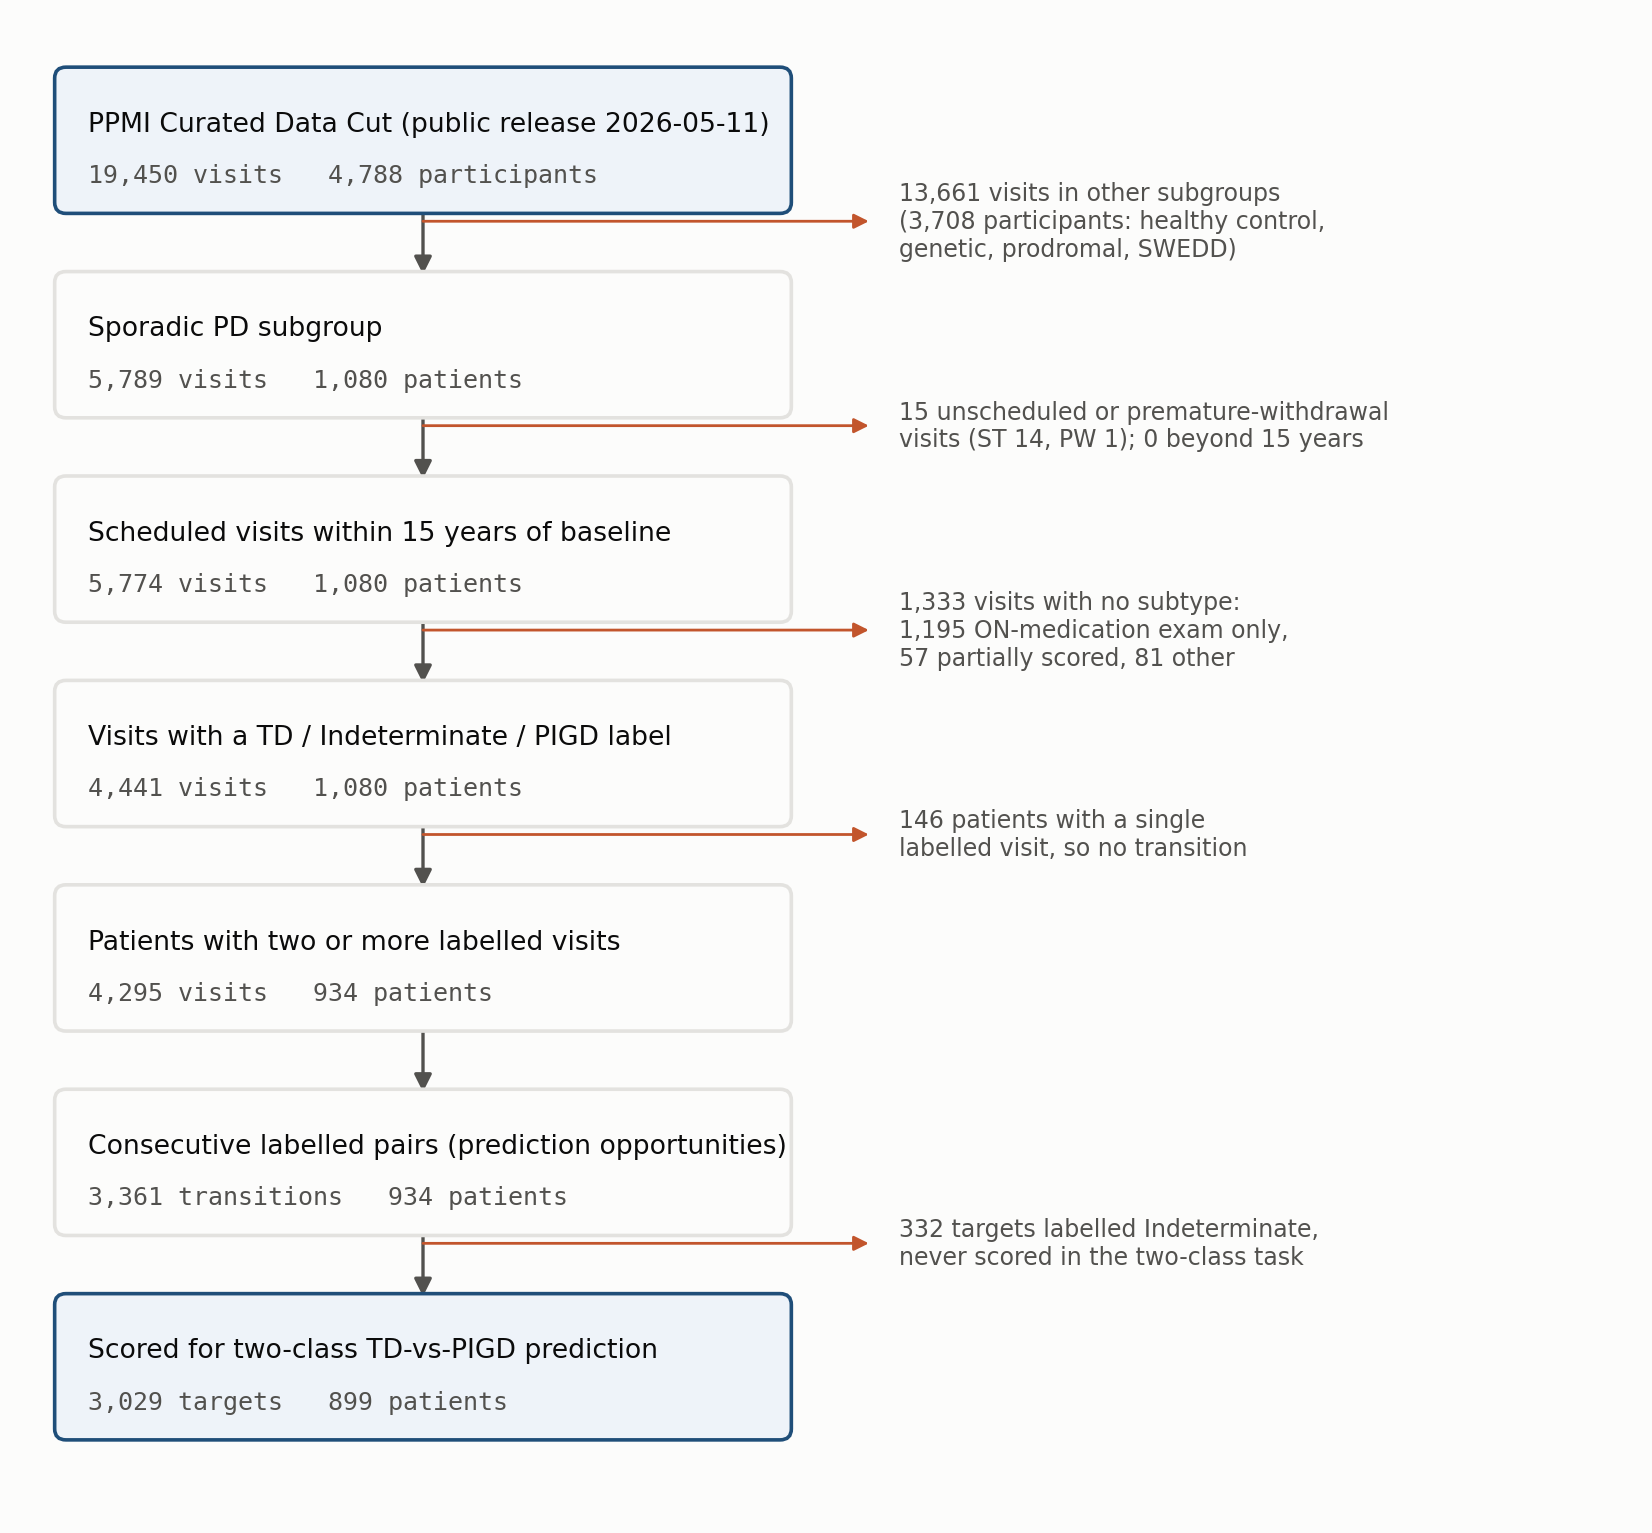
\includegraphics[width=0.84\textwidth]{f01_flow.png}
\caption{Participant flow from the curated data cut to the evaluation set, with
every exclusion counted. The dominant cause of label loss is the OFF-medication
requirement rather than an incomplete examination: 1,195 of 1,333 unlabelled
visits (89.6\%) carried only an ON-medication Part III examination. The final box
is the two-class evaluation set used in the secondary analyses of
Section~\ref{sec:richer}; the three-class analyses use the 3,361 transitions of
the box above it.}
\label{fig:flow}
\end{figure}

\begin{table}[t]
\centering
\caption{Cohort characteristics. Continuous variables are measured at the
participant's first visit and reported as median (interquartile range). The
subtype distribution at the first visit is over the 1,076 first visits that carry
a label. The modelling cohort is the subset of patients contributing at least one
visit-to-visit transition.}
\label{tab:cohort}
\small
\begin{tabular}{@{}lrr@{}}
\toprule
 & Full cohort & Modelling cohort \\
Characteristic & ($\geq 1$ labelled visit) & ($\geq 2$ labelled visits) \\
\midrule
Patients, $n$                               & 1,080 & 934 \\
Labelled visits, $n$                        & 4,441 & 4,295 \\
Labelled visits per patient                 & 3 (2--5) & 4 (3--6) \\
Follow-up, y                                & 3.0 (1.4--5.1) & 3.1 (2.1--6.9) \\
Interval between labelled visits, y         & \multicolumn{2}{c}{1.00 (1.00--1.16)} \\
\addlinespace[2pt]
Male, $n$ (\%)                              & 709 (65.6) & 615 (65.8) \\
Age at baseline, y                          & 64.1 (57.1--70.1) & 63.8 (56.8--69.7) \\
Education, y                                & 16 (14--18) & 16 (14--18) \\
Disease duration at baseline, y             & 0.5 (0.3--1.0) & 0.5 (0.3--1.0) \\
Hoehn \& Yahr stage                         & 2.0 (1.0--2.0) & 2.0 (1.0--2.0) \\
MDS-UPDRS Part I                            & 5 (3--9) & 5 (3--9) \\
MDS-UPDRS Part II                           & 5 (3--9) & 5 (3--9) \\
MDS-UPDRS Part III (OFF)                    & 21 (15--28) & 21 (15--28) \\
MoCA                                        & 27 (26--29) & 27 (26--29) \\
RBDSQ                                       & 3 (2--6) & 3 (2--6) \\
SCOPA-AUT                                   & 9 (6--13) & 9 (6--13) \\
UPSIT                                       & 23 (16--28) & 22 (16--28) \\
DaTscan putamen SBR, bilateral              & 0.7 (0.6--0.9) & 0.7 (0.6--0.9) \\
\addlinespace[2pt]
Tremor subscore $T$ (11 items)              & 0.5 (0.3--0.8) & 0.5 (0.3--0.8) \\
PIGD subscore $P$ (5 items)                 & 0.2 (0.0--0.4) & 0.2 (0.0--0.4) \\
Ratio $r = T/P$, where defined              & 1.8 (0.9--2.7) & 1.8 (0.9--2.8) \\
Visits with $r$ undefined ($P = 0$), $n$ (\%) & 725 (16.3) & 692 (16.1) \\
\midrule
\multicolumn{3}{@{}l}{\textit{Subtype at the first labelled visit}} \\
\quad Tremor dominant                       & 772 (71.7\%) & 676 (72.5\%) \\
\quad Indeterminate                         & 109 (10.1\%) & 99 (10.6\%) \\
\quad PIGD                                  & 195 (18.1\%) & 157 (16.8\%) \\
\addlinespace[2pt]
\multicolumn{3}{@{}l}{\textit{Subtype over all labelled visits}} \\
\quad Tremor dominant                       & 2,891 (65.1\%) & --- \\
\quad Indeterminate                         & 441 (9.9\%) & --- \\
\quad PIGD                                  & 1,109 (25.0\%) & --- \\
\bottomrule
\end{tabular}

\end{table}

\subsection{Missingness and exclusions}
Labels were not imputed; all analyses used complete cases. Of the 1,333 cohort
visits without a subtype, 1,195 (89.6\%) had only an ON-medication Part III
examination and were excluded by the medication-state rule of
Section~\ref{sec:construction}; 65 had no Part III record; 57 had an examination
that was recorded but incomplete; and 16 had a complete Part III but an
incomplete Part II. The dominant mechanism is therefore treatment-related, and
the loss is not random: unlabelled visits came overwhelmingly from treated
participants later in follow-up (median 5.0 years from baseline against 2.0;
96.8\% on antiparkinsonian medication against 57.9\%). The analysed sample is
consequently weighted towards earlier, untreated follow-up, which attenuates
rather than exaggerates observed progression.

\subsection{Visits at which the ratio is undefined}
\label{sec:undefined}
The ratio $r = T/P$ of Section~\ref{sec:rule} is undefined when the PIGD subscore
$P$ is zero. Among all 4,441 labelled visits this occurs at \textbf{725 visits
(16.3\%)}; among the 4,295 labelled visits contributed by the 934 patients of the
modelling cohort it occurs at \textbf{692 visits (16.1\%)}. These visits are
overwhelmingly tremor dominant: of the 725, 665 are TD (a patient with some
tremor and no recorded postural or gait impairment) and 60 are the doubly
degenerate case $T = P = 0$, classified Indeterminate.

This matters for the interpretation of every analysis that models the ratio. The
hierarchical Bayesian growth model and the ratio Gaussian process are defined on
$r$ and cannot use these visits at all, whereas the Markov models, the hidden
Markov model and the subscore models retain them. \textbf{The ratio-based subset
is not a random subset of the cohort}: it systematically excludes the most
strongly tremor-dominant assessments, so quantities estimated on it are
conditioned on the presence of some postural or gait impairment and should not be
read as cohort-wide. The share of labelled visits at which the ratio is defined
also rises with follow-up, from 0.74 in study year 0 to above 0.95 after year
eight, so the ratio cohort is additionally weighted towards later visits. Where a
comparison spans a ratio model and a non-ratio model, we restrict it to the
transitions both can score and say so.

% ====================================================================
\section{The Motor Subtype Label and How It Is Constructed}
\label{sec:construction}
% ====================================================================

Because the central question of this paper concerns the label rather than any
model, we treat the label's construction as a result in its own right and report
it before the methods.

\subsection{The classification rule}
\label{sec:rule}
The \emph{tremor score} $T$ is the mean of eleven MDS-UPDRS items (2.10;
3.15a--b; 3.16a--b; 3.17a--e; 3.18) and the \emph{PIGD score} $P$ the mean of five
(2.12, 2.13, 3.10, 3.11, 3.12), following \citet{stebbins2013}. Writing
$r = T/P$, the subtype at a visit is
\begin{equation}
\mathrm{subtype} =
\begin{cases}
\TD,   & r \geq 1.15 \ \text{ or } (P = 0,\ T > 0),\\[2pt]
\PIGD, & r \leq 0.90,\\[2pt]
\Ind,  & \text{otherwise.}
\end{cases}
\label{eq:rule}
\end{equation}
The final branch covers $0.90 < r < 1.15$ and the doubly degenerate case
$T = P = 0$. The band is open at both ends, so a ratio falling exactly on a
threshold is assigned to the outer class, and the two degenerate cases are
handled explicitly rather than by division.

\subsection{Three data-handling decisions that change the label}
First, PPMI records ``unable to rate'' as the sentinel value 101 \emph{in the
same numeric field as a valid 0--4 rating}; every value outside the valid range
was blanked before any mean was taken. This is not a rounding concern: one such
value among the five PIGD items lifts their mean to roughly 20 and reclassifies a
tremor-dominant visit as PIGD. Second, a subscore was set to missing if
\emph{any} constituent item was missing, matching PPMI's own derivation. Third,
the classification uses the \emph{OFF-medication or untreated} examination,
because levodopa suppresses tremor and scoring ON-state examinations would
manufacture apparent PIGD transitions that are pharmacological rather than
pathological. Where a visit carried more than one eligible Part III examination,
the record with the fewest missing items was retained.

\subsection{What the construction implies}

Table~\ref{tab:construction} reports four audits of the label's construction.

\paragraph{The label is reconstructed exactly, and validates against PPMI's own
derivations.} Rebuilding the item sums from the raw item tables matched the
frozen panel at all 5,774 visits, with zero mismatches in the tremor score, the
PIGD score or the label. Agreement with PPMI's own two-class derived label was
4,431 of 4,431 (100.00\%), and with a three-class label in an archived release
covering 390 participants, 1,595 of 1,597 (99.87\%). Nothing that follows is an
artefact of our implementation of the rule.

\paragraph{A quarter of same-visit labels move with the examination state.}
Scoring the same visit from the OFF-medication and the ON-medication examination
gives the same label at only \textbf{75.2\%} of the 2,343 pairs that carry both
(714 patients), and at 72.1\% when the label is built from the Part III items
alone. The ON examination's tremor item sum is a median of 2 points lower than
the OFF examination's (10th to 90th percentile $-7$ to $0$) against a median
difference of 0 for the PIGD sum. This comparison confounds medication response
with time of day, examination order and rater, so it is not a test--retest
reliability coefficient; but it bounds the within-visit stability of the label at
about three quarters, and it does so without reference to any model or to any
change in the patient.

\paragraph{The ratio lives on a lattice, and the Indeterminate band is thinner
than the lattice's own spacing.} Because $T$ is a mean of eleven integer ratings
and $P$ a mean of five, $r$ takes values on a lattice rather than a continuum
(Figure~\ref{fig:lattice}). Inside a band only $0.25$ wide, just \textbf{eleven}
attainable values occur among the 381 Indeterminate visits with a defined ratio,
and two of them dominate: 198 visits (52.0\%) sit at $r = 0.9091$ and 100
(26.2\%) at $r = 1.1364$, which are 0.009 and 0.014 from the respective
thresholds (Figure~\ref{fig:attainable}). Every Indeterminate visit in the cohort
is one item point away from another label. The PIGD item sum is zero at 16.3\% of
labelled visits and the tremor sum at 7.2\%, so a substantial part of the panel
sits on the degenerate edges of the lattice.

\begin{figure}[t]
\centering
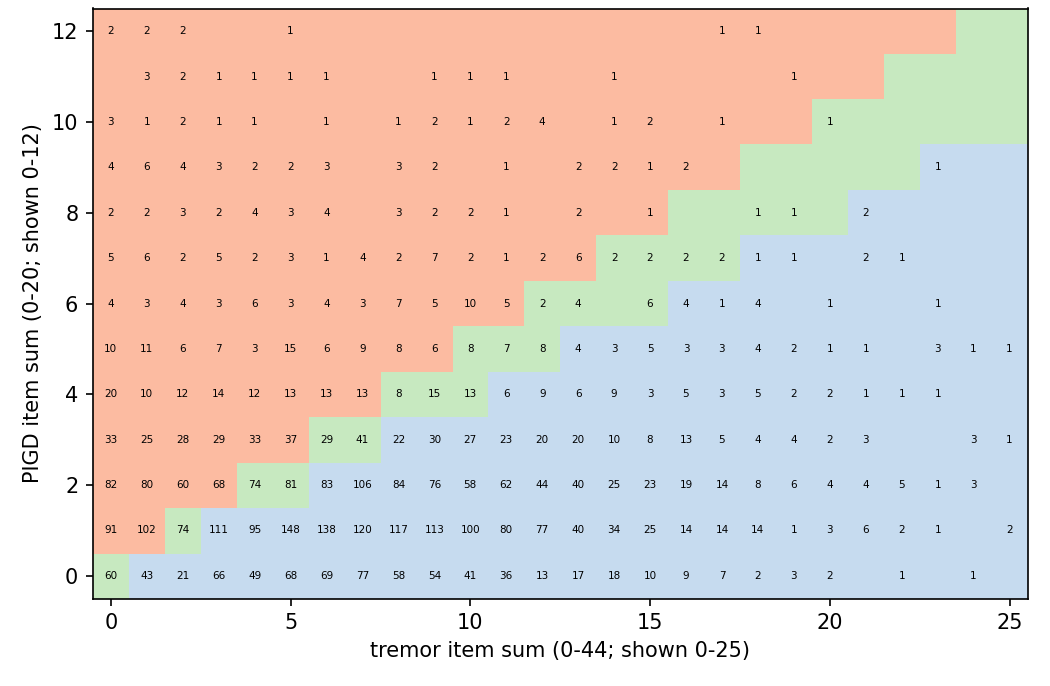
\includegraphics[width=0.80\textwidth]{f02_lattice.png}
\caption{The label as a function of the two integer item sums. Each cell is an
attainable combination of the tremor item sum (horizontal) and the PIGD item sum
(vertical), shaded by the class that~\eqref{eq:rule} assigns to it --- blue TD,
green Indeterminate, red PIGD --- and annotated with the number of labelled
visits it holds. The Indeterminate region is a thin diagonal strip one cell wide
over most of its length, so every Indeterminate visit is one item point from
another label.}
\label{fig:lattice}
\end{figure}

\begin{figure}[t]
\centering
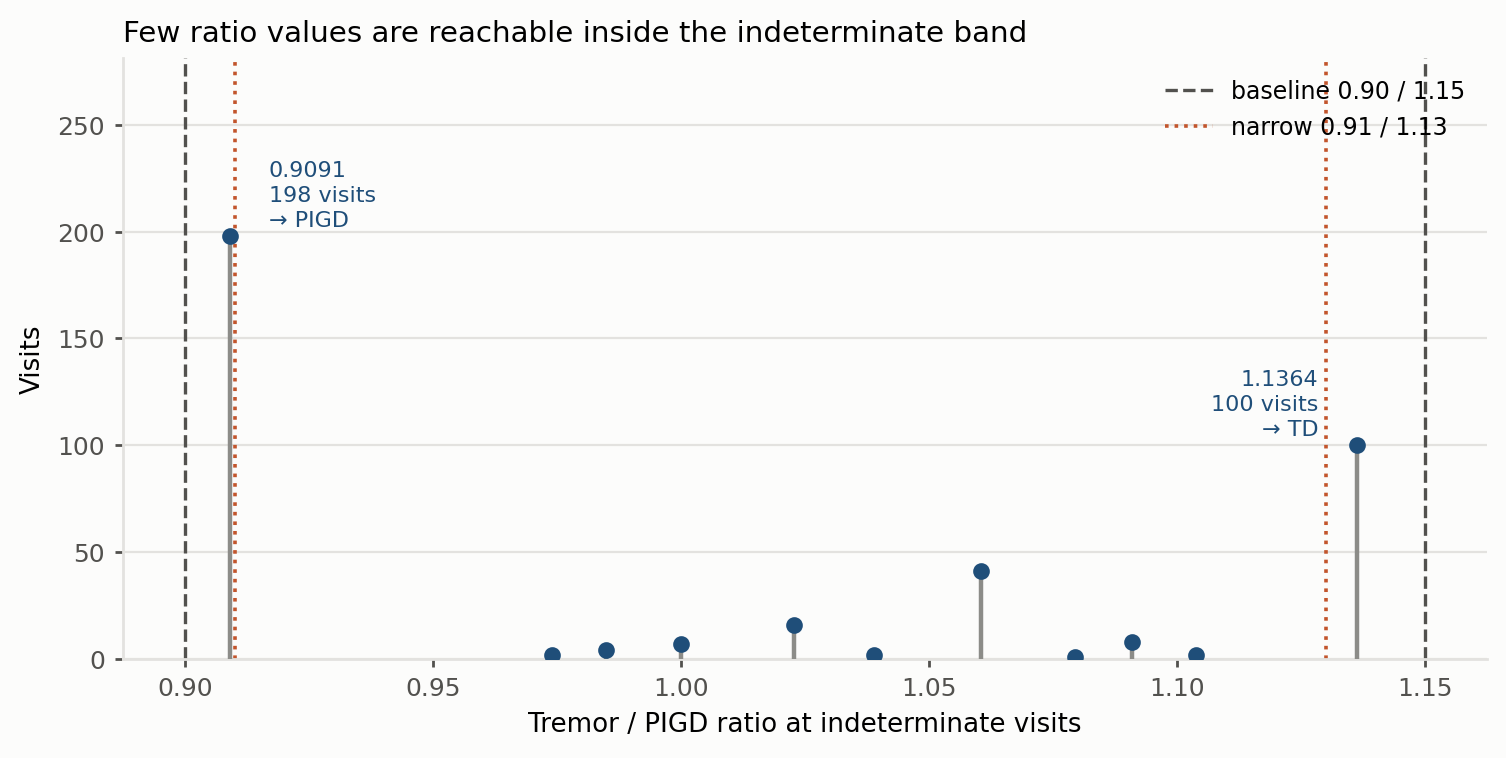
\includegraphics[width=0.84\textwidth]{f03_attainable.png}
\caption{Attainable values of the ratio inside the Indeterminate band. Each point
is one attainable value of $r = T/P$ and its height the number of labelled visits
taking it; dashed lines are the thresholds of~\eqref{eq:rule} and dotted lines
the perturbed rule. Of the 381 Indeterminate visits with a defined ratio, 78\%
sit at the two values nearest the thresholds, so moving the thresholds by less
than the spacing of the lattice moves both values across.}
\label{fig:attainable}
\end{figure}

\paragraph{A threshold perturbation smaller than the lattice spacing relabels a
fifth of patients.} Rebuilding the entire panel under a perturbed rule that moves
both thresholds inward by 0.01 and 0.014 (PIGD if $r < 0.91$, TD if $r > 1.13$)
relabels \textbf{298 of 4,441 labelled visits (6.71\%), every one of them out of
the Indeterminate class}. No TD or PIGD visit moves. The Indeterminate class
falls from 441 visits to 143, a reduction of 67.6\%, with 198 becoming PIGD and
100 becoming TD --- exactly the two dominant lattice values, so the entire effect
is two attainable values crossing a line that moved by less than the gap between
adjacent values. Measured over patients rather than visits, the perturbation
touches \textbf{235 of 1,080 (21.76\%)}, and agreement with PPMI's own derived
labels falls from 1.000 to 0.977 (two-class) and from 0.999 to 0.929
(three-class). This is a deterministic recomputation on a fixed panel rather than
an estimate from a sample, so no uncertainty interval is reported and none would
be appropriate; neither rule is treated as correct.

\begin{table}[t]
\centering
\caption{Audits of the label's construction. Panels (a) and (b) establish that the
label is reproduced exactly from the items but depends heavily on which
examination is scored; panels (c) and (d) establish that the Indeterminate band
is narrower than the resolution of the quantity it is applied to.}
\label{tab:construction}
\small
\begin{tabular}{@{}llr@{}}
\toprule
Property & Quantity & Value \\
\midrule
\multicolumn{3}{@{}l}{\textit{(a) Reconstruction from the raw items}}\\
 & Visits reconstructed exactly ($T$, $P$ and label) & 5,774 of 5,774 \\
 & Agreement with PPMI's two-class derived label & 4,431 of 4,431 (100.00\%) \\
 & Agreement with an archived three-class derived label & 1,595 of 1,597 (99.87\%) \\
\addlinespace[3pt]
\multicolumn{3}{@{}l}{\textit{(b) Dependence on the examination state (same visit, OFF vs ON)}}\\
 & Label agreement, all 16 items & 0.7516 \\
 & Label agreement, Part III items only & 0.7208 \\
 & Same-visit OFF/ON pairs with both labels & 2,343 (714 patients) \\
 & Median ON${-}$OFF tremor item sum (10th--90th pct) & $-2$ ($-7$ to $0$) \\
 & Median ON${-}$OFF PIGD item sum (10th--90th pct) & $\phantom{-}0$ ($-1$ to $0$) \\
\addlinespace[3pt]
\multicolumn{3}{@{}l}{\textit{(c) The integer lattice inside the Indeterminate band}}\\
 & Indeterminate visits with a defined ratio & 381 \\
 & Distinct attainable ratio values they take & 11 \\
 & At $r = 0.9091$ (0.009 from the PIGD threshold) & 198 (52.0\%) \\
 & At $r = 1.1364$ (0.014 from the TD threshold) & 100 (26.2\%) \\
 & PIGD item sum $=0$ among labelled visits & 16.3\% \\
 & Tremor item sum $=0$ among labelled visits & 7.2\% \\
\addlinespace[3pt]
\multicolumn{3}{@{}l}{\textit{(d) Sensitivity to threshold placement (perturbed rule $r<0.91$ / $r>1.13$)}}\\
 & Labelled visits relabelled & 298 of 4,441 (6.71\%) \\
 & \quad of which leaving the Indeterminate class & 298 (100\%) \\
 & \quad TD or PIGD visits moved & 0 \\
 & Patients with at least one relabelled visit & 235 of 1,080 (21.76\%) \\
 & Indeterminate visits before $\to$ after & 441 $\to$ 143 ($-67.6$\%) \\
 & Agreement with PPMI two-class label, base $\to$ perturbed & 1.000 $\to$ 0.977 \\
 & Agreement with PPMI three-class label, base $\to$ perturbed & 0.999 $\to$ 0.929 \\
\bottomrule
\end{tabular}

\end{table}

\paragraph{What follows from this section.} Two properties of the label are fixed
before any model is fitted and cannot be removed by a better predictor: the label
of a visit depends substantially on which examination is scored, and the
Indeterminate class is an arithmetically fragile strip whose membership is
decided by differences smaller than one item point. Both are properties of the
measurement, and both bound what any model of the label can achieve.

% ====================================================================
\section{Research Questions}
% ====================================================================

The programme reported here was organised around six questions, in order.

\begin{enumerate}
\itemsep2pt
\item \textbf{How does the recorded label behave over follow-up?} How often is an
observed change undone at the next visit, how does the estimated conversion
incidence depend on the definition of a conversion, does the transition structure
depend on the elapsed interval, and is the recorded label first-order Markov?
(Section~\ref{sec:dynamics}.)

\item \textbf{Does a generative model of the underlying ratio reproduce the
label's dynamics?} If the ratio follows a hierarchical growth model with
heavy-tailed slopes and residuals, do label sequences simulated from it reproduce
the observed Indeterminate share, reversion rates and clustering?
(Section~\ref{sec:ppc}.)

\item \textbf{Does a latent state predict the next recorded label better than a
chain in the label itself, and do more latent states help?}
(Section~\ref{sec:discrete}.)

\item \textbf{Does modelling the continuous quantity the label is cut from
predict the label better?} The ratio and the two subscores, under parametric
growth models, Gaussian processes and mixed models, with the label derived
afterwards through the unchanged rule. (Section~\ref{sec:continuous}.)

\item \textbf{When every family is placed under one decision rule and one case
list, how far apart are they, and where does each model's advantage over a
trivial rule come from?} (Section~\ref{sec:harmonised}.)

\item \textbf{Does a richer observation of the patient help, and if so on which
metric?} Ten clinical measurements through a discrete latent state and through a
continuous profile, and the ratio band inside the latent-state model's own
observation alphabet. (Section~\ref{sec:richer}.)
\end{enumerate}

A seventh question runs through the programme and is settled in
Section~\ref{sec:ceiling}: if the accuracy ceiling is real, is it explained by too
little history, by the training regime, by disease stage, or by heterogeneity
across patients?

% ====================================================================
\section{Methods}
\label{sec:methods}
% ====================================================================

\subsection{The longitudinal prediction task}
\label{sec:task}
Visits were ordered within patient by elapsed time from that patient's first
visit. Unlabelled visits were removed before pairing, so a missing year does not
break a sequence; a \emph{transition} is a pair of consecutive \emph{labelled}
visits, carrying the actual elapsed interval between them.

The task is: given a patient's history up to and including visit $k$, and the
elapsed interval $\Delta$ to visit $k+1$, predict the subtype recorded at visit
$k+1$. The unit of prediction is one transition, and the evaluation set is the
3,361 transitions of Section~\ref{sec:data}.

What is available at prediction time is the patient's own labelled history
$y_1,\dots,y_k$ (or, for the continuous models, the subscore, ratio or
measurement history), the elapsed times between those visits, and the interval
$\Delta$ to the target visit. The model is told \emph{when} the next visit
happens, not what is recorded at it. This is the usual convention for panel data
but is an assumption worth stating: no result here addresses when a patient will
next be seen, and all transition probabilities are conditional on the next visit
occurring.

\subsection{Observed-label Markov models}
Two specifications treat the recorded label itself as the state, so that the
state space is $\mathcal{S} = \{\TD, \Ind, \PIGD\}$ and no latent structure is
posited.

The \emph{discrete-time chain} estimates a row-stochastic matrix $A$ with
$A_{ab} = \Pr(y_{k+1} = b \mid y_k = a)$ from the observed pairs by maximum
likelihood, ignoring the elapsed interval. Its assumption is that the next label
depends on the current one and on nothing else, including the time between
visits.

The \emph{continuous-time chain} relaxes the second half of that assumption. It
estimates a generator $Q$ with non-negative off-diagonal entries and rows summing
to zero, giving
\begin{equation}
\Pr(y_{k+1} = b \mid y_k = a,\ \Delta) = \bigl[\exp(Q\Delta)\bigr]_{ab},
\label{eq:ctmc}
\end{equation}
where $\exp(\cdot)$ is the matrix exponential. Off-diagonal rates are
parameterised as $\exp(\theta)$ to keep them positive. This specification is
interval-aware but still first-order in the observed label.

Whether that first-order assumption holds is testable without fitting either
model, by asking whether the next label is conditionally independent of the
previous one given the current one. We test this on consecutive triples with a
$\chi^2$ test of independence, separately for each current state
(Section~\ref{sec:dynamics}).

\subsection{Hidden Markov model with a misclassification matrix}
\label{sec:hmm}
The hidden Markov model separates what is recorded from what is modelled as
evolving. A latent state $X(t) \in \mathcal{S}$ evolves as a continuous-time
Markov chain with generator $Q$, and what is observed at visit $k$ is not
$X(t_k)$ but a noisy reading $Y_k$ related to it by a misclassification matrix
$E$,
\begin{equation}
E_{ab} = \Pr(Y_k = b \mid X(t_k) = a), \qquad \sum_b E_{ab} = 1 .
\label{eq:emission}
\end{equation}
This is the classification-error construction of~\citet{jackson2003}. The
likelihood of one patient's whole sequence marginalises over every latent path by
the forward algorithm,
\begin{equation}
L = \pi^{\!\top} \! \operatorname{diag}(E_{\cdot y_1})
    \prod_{k=2}^{K} \exp\!\bigl(Q \Delta_{k-1}\bigr)
    \operatorname{diag}(E_{\cdot y_k})\, \mathbf{1},
\label{eq:forward}
\end{equation}
and a prediction for visit $k+1$ is obtained by filtering the history to a
posterior over $X(t_k)$, propagating it through $\exp(Q\Delta)$, and passing it
through $E$. Specifications with three, four and five latent states were fitted
by maximum likelihood with deterministic restarts.

A constraint is required. Left unconstrained, the maximum-likelihood solution is
degenerate and identical across random restarts: the latent Indeterminate state
emits uniformly and PIGD becomes absorbing at the parameter boundary. We
therefore require each state to be recorded correctly more often than not,
$E_{aa} \geq 0.5$. The consequences of this constraint, and the behaviour of the
unconstrained and larger specifications, are reported in
Supplementary~\ref{sup:hmm}.

The latent states of this model are a modelling device. They are estimated solely
from the sequence of recorded labels and their timings, and nothing in this
design identifies them with clinically validated phenotypes. We refer to them as
latent states throughout and do not interpret them as independently confirmed
subtypes.

\subsection{Hierarchical Bayesian growth model of the ratio}
\label{sec:hb}
The growth model abandons the discrete label and models the continuous quantity
the label is cut from. For patient $i$ at time $t_{ij}$ years from that patient's
first visit,
\begin{align}
r_{ij} &= \bigl(\beta_0 + b_{0i}\bigr) + \bigl(\beta_1 + b_{1i}\bigr) t_{ij} + \varepsilon_{ij},
\label{eq:hb}\\[2pt]
b_{0i} &\sim \mathcal{N}(0, \tau_0^2), \quad
b_{1i} \sim \mathcal{N}(0, \tau_1^2), \quad
\varepsilon_{ij} \sim \mathcal{N}(0, \sigma^2),
\nonumber
\end{align}
with $\beta_0, \beta_1$ the population intercept and slope, $b_{0i}, b_{1i}$
patient-level deviations, and $\varepsilon_{ij}$ residual variation. The model was
fitted by Gibbs sampling under weakly informative priors on 2,426 ratio
observations from 573 training patients.

Two points of specification matter. First, $\sigma$ is the \emph{total} residual
SD. Separate observation and process terms, both additive on the same
observation, are not separately identifiable, so only their sum is estimated;
this is a limitation of the specification, not a choice, and it means the model
cannot separate measurement error from true fluctuation. Second, the model is
defined on $r$ and therefore uses only visits at which $r$ is defined
(Section~\ref{sec:undefined}).

Student-t variants replacing the Gaussian slopes, the Gaussian residuals, or both
were fitted and compared over seven patient splits
(Supplementary~\ref{sup:studentt}).

A subtype prediction is derived by applying the unchanged rule~\eqref{eq:rule} to
the predictive distribution of $r$, which makes the relationship between the
residual spread $\sigma$ and the width of the Indeterminate band directly
interpretable.

\subsection{Gaussian process regression}
\label{sec:gp}
Gaussian process regression~\citep{rasmussen2006} replaces the parametric linear
trend of~\eqref{eq:hb} with a distribution over functions. For a patient's
trajectory $f(t)$ we take $f \sim \mathcal{GP}\bigl(m(t), k(t,t')\bigr)$ with a
fitted linear mean function $m(t)$ and Gaussian observation noise, and compare
four covariance functions:
\begin{align*}
K_0:&\quad k = \sigma_c^2 + \sigma_\ell^2\, t t'  &&\text{(constant + linear)}\\
K_1:&\quad k = \sigma_c^2 + \sigma_f^2 \exp\!\bigl(-\tfrac{(t-t')^2}{2\ell^2}\bigr) &&\text{(constant + squared exponential)}\\
K_2:&\quad k = \sigma_c^2 + \sigma_\ell^2\, t t' + \sigma_f^2 \exp\!\bigl(-\tfrac{(t-t')^2}{2\ell^2}\bigr) &&\text{(both)}\\
K_3:&\quad k = \sigma_c^2 + \sigma_\ell^2\, t t' + \text{Mat\'ern-}3/2 &&\text{(rougher alternative)}
\end{align*}
$K_0$ is the Gaussian process analogue of a linear trend and is the natural
comparator for the growth model; $K_1$ is the flexible alternative. The
comparison $K_1$ against $K_0$ asks whether departures from a straight line carry
predictive signal, and $K_3$ against $K_1$ asks whether the trajectory is rougher
than a squared-exponential kernel allows.

Gaussian processes were fitted to three targets: the ratio $r$, and the tremor
and PIGD subscores modelled separately. The subscore models were additionally
fitted in a jointly-covarying (multi-output) form, in which a coregionalisation
block couples the two outputs, with its diagonal counterpart as the nested
control.

\subsection{Mixed models of the subscores}
A joint bivariate linear mixed model on the two subscores, with correlated
patient-level random intercepts, provides an interpretable parametric comparator
(Supplementary~\ref{sup:subscore}). A time-varying variant replaces the constant
population slope with a linear spline in time from baseline, with knots at two
and five years, to ask whether the rate of change of each subscore is constant
over follow-up (Supplementary~\ref{sup:temporal}).

\subsection{Richer observations of the patient}
\label{sec:methods-richer}
Three specifications widen the observation beyond the subtype label.

A \emph{discrete latent clinical state} replaces the three-state label alphabet
with a continuous-time hidden Markov model whose Gaussian emission is over ten
standardised clinical measurements, with the state count selected on a
development set.

A \emph{continuous nine-domain profile} gives every patient, in each of nine
clinical domains (bradykinesia/rigidity, tremor, PIGD, MDS-UPDRS Parts I and II,
MoCA, GDS, SCOPA-AUT and ESS), two numbers filtered from their own history by a
continuous-time local linear trend model: a \emph{level} and a \emph{rate of
change}. Levodopa-equivalent daily dose enters as an input to the observation
equation rather than as a domain, so that ``has started treatment'' is not one of
the coordinates. Inference is a Kalman filter, so the state after visit $k$ is a
function of visits $0,\dots,k$ and nothing else; the absence of future
information is a structural property of the recursion rather than a convention to
be policed.

A \emph{ratio-banded observation alphabet} keeps the latent-state model of
Section~\ref{sec:hmm} unchanged and widens only what it observes: the observation
at a visit becomes the pair (subtype, ratio band), where the band discretises $r$
at a fixed width, giving a joint alphabet of up to 73 categories. Because the
latent process and the decision rule are untouched, any change in performance is
attributable to the observation alone. Band widths of 0.05, 0.10, 0.20, 0.30 and
0.50 were swept.

\subsection{Baselines}
The canonical baseline is \textbf{persistence}: name the currently recorded
label. It is the trivial rule a clinician would use, it has no parameters, and it
needs no subscores. Four further reference points are kept clearly separate from
it: subscore last-observation-carried-forward, a patient-mean subscore, a
population-mean subscore, and a marginal null that always predicts the majority
class. A first-visit multinomial model with baseline covariates provides a
no-history reference (Supplementary~\ref{sup:firstvisit}).

% ====================================================================
\section{Evaluation Protocol}
\label{sec:evaluation}
% ====================================================================

\subsection{Patient-level validation}
All primary models were validated by \textbf{leave-one-patient-out}
cross-validation. For each of the 934 patients in turn, the model is refitted
from scratch on all other patients and then used to predict that patient's
recorded subtypes one visit at a time. \emph{No visit of the held-out patient
enters the fit}, and each prediction uses only that patient's own earlier visits
as history. This yields 3,361 held-out predictions from 934 patients for every
specification, on the same case list.

The structural point is that the holdout is at the level of the \emph{patient},
not the visit. Because one patient contributes several correlated transitions,
holding out a visit while training on its neighbours from the same patient would
leak information; holding out the patient removes that channel entirely.

A battery of ten checks was asserted at run time on every saved prediction row:
that every patient is held out exactly once; that the held-out patient is the
patient being predicted; that every fold trained on all other patients; that the
prediction count equals the transition count; that the history is strictly the
visits before the target; that the target visit is always later than the current
visit; that probabilities sum to one; that the predicted class is the argmax;
that the confusion-matrix totals equal the prediction count; and that every fit
converged. All ten passed for the three-state specifications. The history-window
experiments of Section~\ref{sec:ceiling} add a tamper test, which found zero
spurious changes over 934 folds and 11,644 cases.

\subsection{Comparisons that span validation designs}
The nine-domain profile is validated by repeated patient-level five-fold
cross-validation (four repeats) rather than leave-one-patient-out, because
leave-one-out was measured at roughly 153 seconds per fit. The standardiser,
model parameters and all baselines are refitted inside every fold on training
patients only. Where the profile is compared against a leave-one-patient-out
model, the comparison is made through paired predictions on identical cases, and
the design difference is stated with the result; it favours the
leave-one-patient-out model.

Similarly, the growth model and the ratio Gaussian process cannot score every
transition (Section~\ref{sec:undefined}). Where they are compared against a model
that can, the comparison is restricted to the transitions both can score and the
restricted sample size is reported.

\subsection{Harmonisation of the decision rule}
\label{sec:harmonisation}
The central methodological step in comparing families is that \textbf{every
specification is expressed as a three-class predictive probability vector over
$(\TD, \Ind, \PIGD)$ on the same 3,361 cases, and the predicted class is the
argmax of that vector}. The chains and the hidden Markov models are natively on
this representation; the continuous models are converted by Monte Carlo through
the project's own unmodified classification function --- 10,000 draws per case
from the model's joint predictive distribution, each draw classified
by~\eqref{eq:rule}, and the resulting class frequencies taken as the probability
vector. Common random numbers are used across specifications so that the draws
cancel in paired contrasts. No tuned thresholds and no per-model calibration are
applied.

Two checks bound the cost of this conversion. Halving the number of draws moved
accuracy by at most 0.0015 for any specification, and the vectorised
implementation of~\eqref{eq:rule} was checked against the reference
implementation on 5,000 synthetic cases including 400 both-subscores-zero and 600
PIGD-zero cases (5,000 of 5,000 agreement).

Harmonisation is not cosmetic. The same saved predictions from one Gaussian
process score 0.7298 under a point-estimate label derivation and 0.7566 under the
probability-vector derivation --- a difference larger than the entire spread
between the nine fitted specifications.

\subsection{Metrics}
Models are compared on accuracy, multiclass Brier score, log loss, macro-F1 and
per-class recall; on two-class tasks, additionally on area under the ROC curve,
average precision, partial area under the curve in the operating region
(false-positive rate at most 0.2) and a calibration gap. Accuracy alone is
reported nowhere without a probabilistic companion~\citep{gneiting2007,
vancalster2019}, because on a three-class target with a small middle class the
two can rank specifications in opposite orders. Continuous targets are scored by
mean absolute error (MAE), root mean squared error, continuous ranked probability
score (CRPS), log predictive score and the coverage of the stated 95\% predictive
interval. Because the subscores and the ratio are non-negative while the models
place Gaussian predictive distributions on them, we also report the predictive
mass falling below zero as a diagnostic of misspecification.

\subsection{Uncertainty and its interpretation}
Because one patient contributes several correlated transitions, every interval
reported here is a \textbf{patient-level cluster bootstrap}: patients are drawn
with replacement carrying all of their visits, and every statistic is recomputed
from scratch in each replicate (2,000 draws unless stated; 4,000 for the
fifteen-arm subscore comparison of Supplementary~\ref{sup:subscore}). Paired
contrasts share one resample between the two conditions in every replicate, so
the reported difference and its interval are paired.

Intervals from the hierarchical Bayesian model are \emph{credible} intervals from
the posterior and are labelled as such; all others are bootstrap
\emph{confidence} intervals, and the two are not interchangeable. Where a
deterministic recomputation on a fixed panel is reported --- the threshold
perturbation of Section~\ref{sec:construction} --- no interval is given, because
none would be meaningful.

We report whether an interval excludes zero, which is a statement about
precision, and separately whether a difference is large enough to matter, which
is not. \textbf{An interval that contains zero is a failure to detect a difference
at this sample size; it is not evidence that two models are equivalent, and we do
not treat it as such anywhere in this paper.} Multiplicity is largely uncorrected
across the specifications compared, and analyses described as exploratory were
specified after the predictions were generated.

% ====================================================================
\section{Results}
% ====================================================================

\subsection{How the recorded label behaves over follow-up}
\label{sec:dynamics}

Across the 3,361 transitions, TD was the most persistent recorded state and
Indeterminate by far the least (Figure~\ref{fig:instability}a,
Table~\ref{tab:transitions}). A visit recorded TD was followed by another TD
visit with probability 0.808 (95\% CI 0.788--0.826), and a PIGD visit by another
PIGD visit with probability 0.702 (0.661--0.738). A visit recorded Indeterminate
remained Indeterminate with probability only 0.192 (0.148--0.234), returning to
TD in 0.440 (0.381--0.500) of cases and moving to PIGD in 0.368 (0.318--0.417).
PIGD was not absorbing: 29.8\% of PIGD visits were followed by a non-PIGD
assessment.

\begin{figure}[t]
\centering
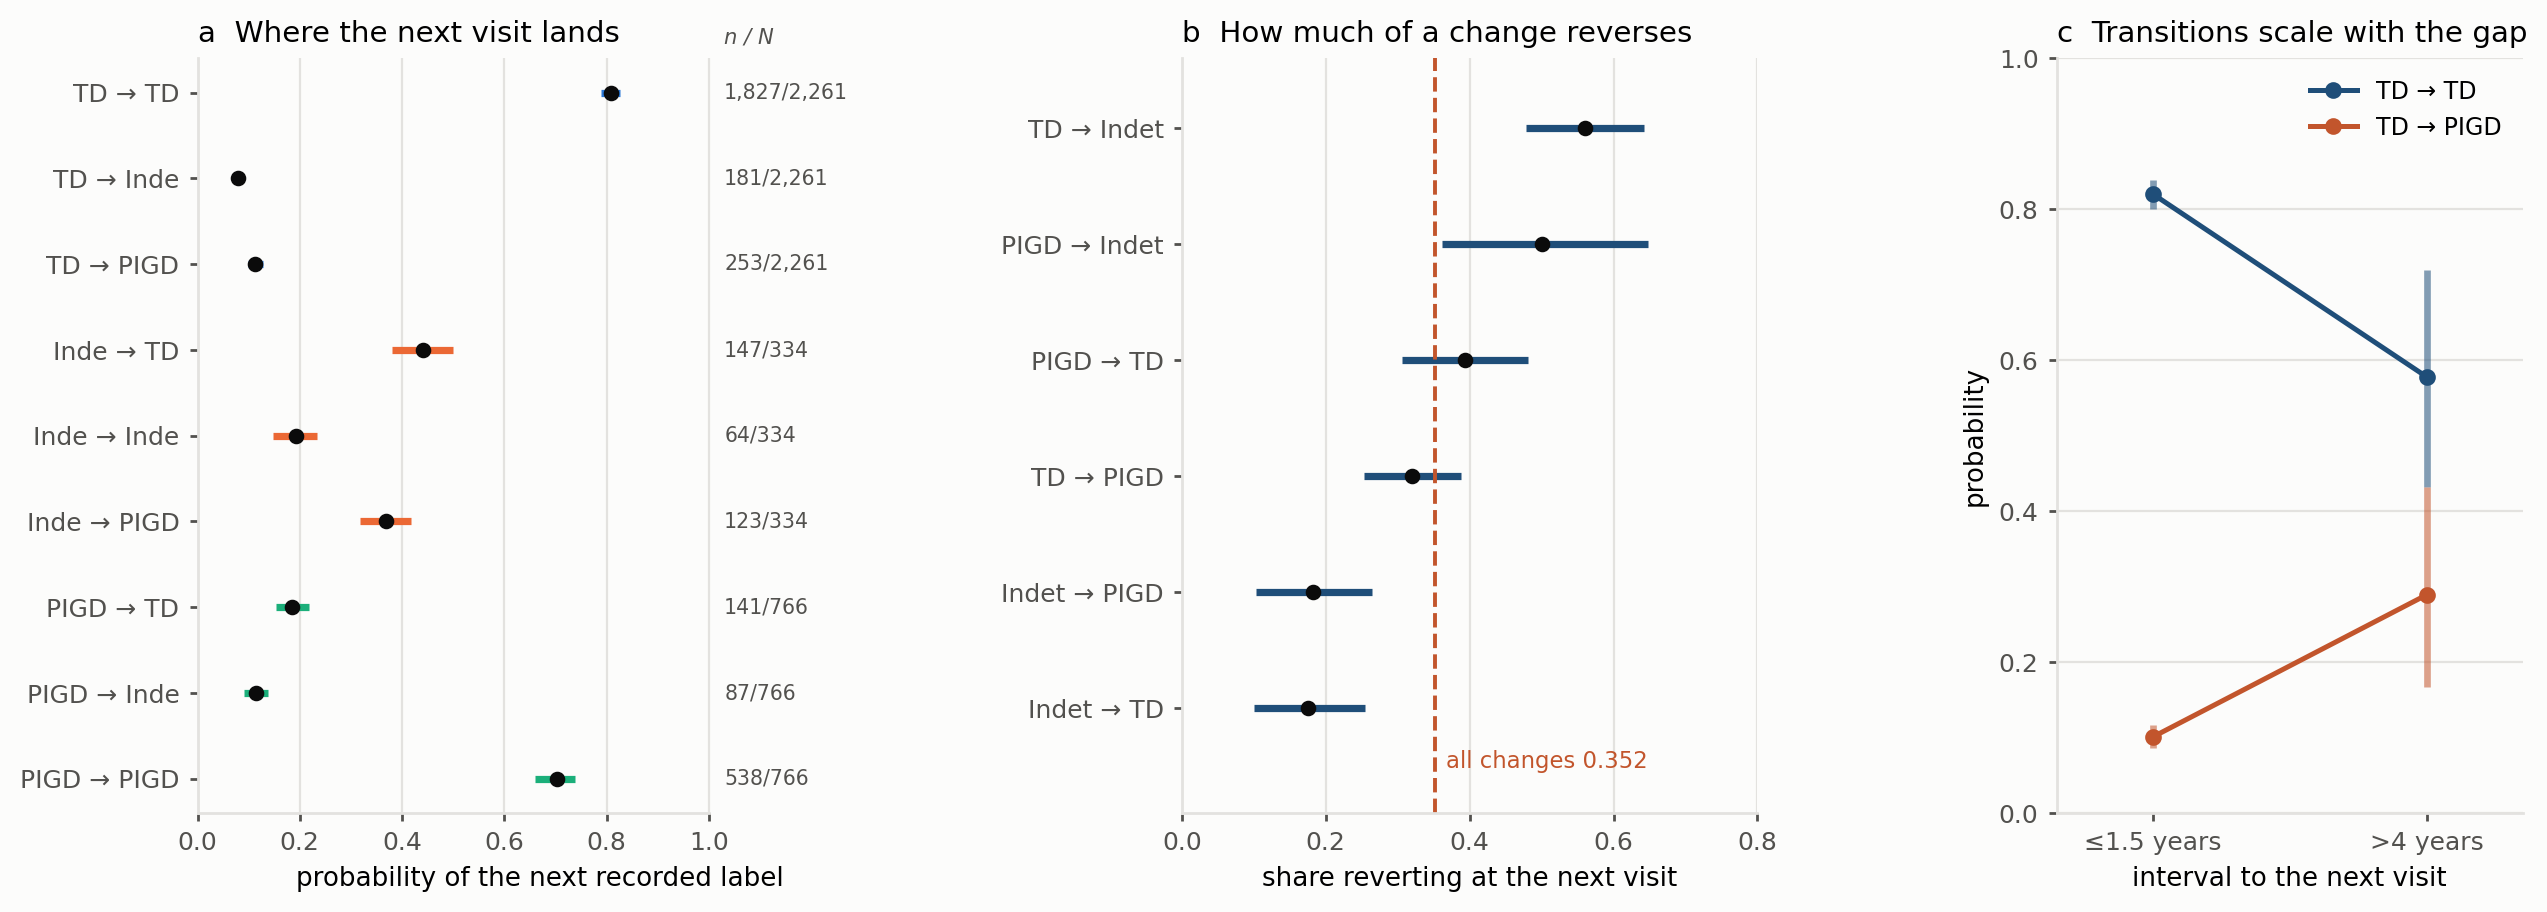
\includegraphics[width=\textwidth]{f04_instability.png}
\caption{The recorded label is unstable, and much of the instability is not
progression. (\textbf{a}) One-step transition probabilities over the 3,361
consecutive labelled visit pairs, with patient-clustered bootstrap 95\%
intervals; the counts at the right are the numerator and denominator of each
estimate. (\textbf{b}) Of every observed change of state, the proportion back at
the origin state one visit later, with the pooled rate of 0.352 marked; changes
into the Indeterminate band revert far more often than changes crossing the full
width of the scale. (\textbf{c}) TD$\to$TD and TD$\to$PIGD probabilities
stratified by the elapsed interval to the next visit.}
\label{fig:instability}
\end{figure}

\begin{table}[t]
\centering
\caption{One-step transition probabilities between consecutive labelled visits,
with patient-clustered bootstrap 95\% intervals over the 934 patients. Rows sum
to one.}
\label{tab:transitions}
\small
\begin{tabular}{@{}llrrl@{}}
\toprule
Subtype at visit $k$ & Subtype at visit $k+1$ & $n$ & $\hat{p}$ & 95\% CI \\
\midrule
TD ($n{=}2{,}261$) & TD & 1,827 & 0.808 & (0.788, 0.826) \\
 & Indeterminate & 181 & 0.080 & (0.068, 0.092) \\
 & PIGD & 253 & 0.112 & (0.098, 0.127) \\
\addlinespace[2pt]
Indeterminate ($n{=}334$) & TD & 147 & 0.440 & (0.381, 0.500) \\
 & Indeterminate & 64 & 0.192 & (0.148, 0.234) \\
 & PIGD & 123 & 0.368 & (0.318, 0.417) \\
\addlinespace[2pt]
PIGD ($n{=}766$) & TD & 141 & 0.184 & (0.153, 0.218) \\
 & Indeterminate & 87 & 0.114 & (0.091, 0.138) \\
 & PIGD & 538 & 0.702 & (0.661, 0.738) \\
\bottomrule
\end{tabular}

\end{table}

\paragraph{A third of observed changes reversed immediately.}
Of 673 observed changes of state, \textbf{35.2\% (31.8--38.8) returned to the
origin state at the following visit} (Figure~\ref{fig:instability}b,
Table~\ref{tab:dynamics}a). Reversion was concentrated in changes involving the
Indeterminate band: TD$\to$Indeterminate reversed in 0.560 (0.478--0.642) of
cases and PIGD$\to$Indeterminate in 0.500 (0.362--0.648), while changes crossing
the full width of the scale reversed less often --- TD$\to$PIGD in 0.320
(0.253--0.388) and PIGD$\to$TD in 0.393 (0.305--0.481).

This is the statistic that separates the two readings of an observed change. A
change undone at the very next assessment is not easily read as phenotypic
progression, and more than a third of changes in this cohort were.

\paragraph{The definition of a conversion dominates its estimated frequency.}
Among the 885 patients not PIGD at their first labelled visit, 263 converted to
PIGD on a single-assessment definition but only 127 when the conversion was
required to hold across two consecutive labelled visits --- a reduction of
\textbf{51.7\% (45.7--57.7)}. Kaplan--Meier cumulative incidence at five years
was 35.3\% (30.8--39.9) under the single-visit definition against 15.3\%
(12.0--19.0) under the sustained one (Figure~\ref{fig:conversion}). The two
definitions differ by roughly a factor of two on the same patients.

\begin{figure}[t]
\centering
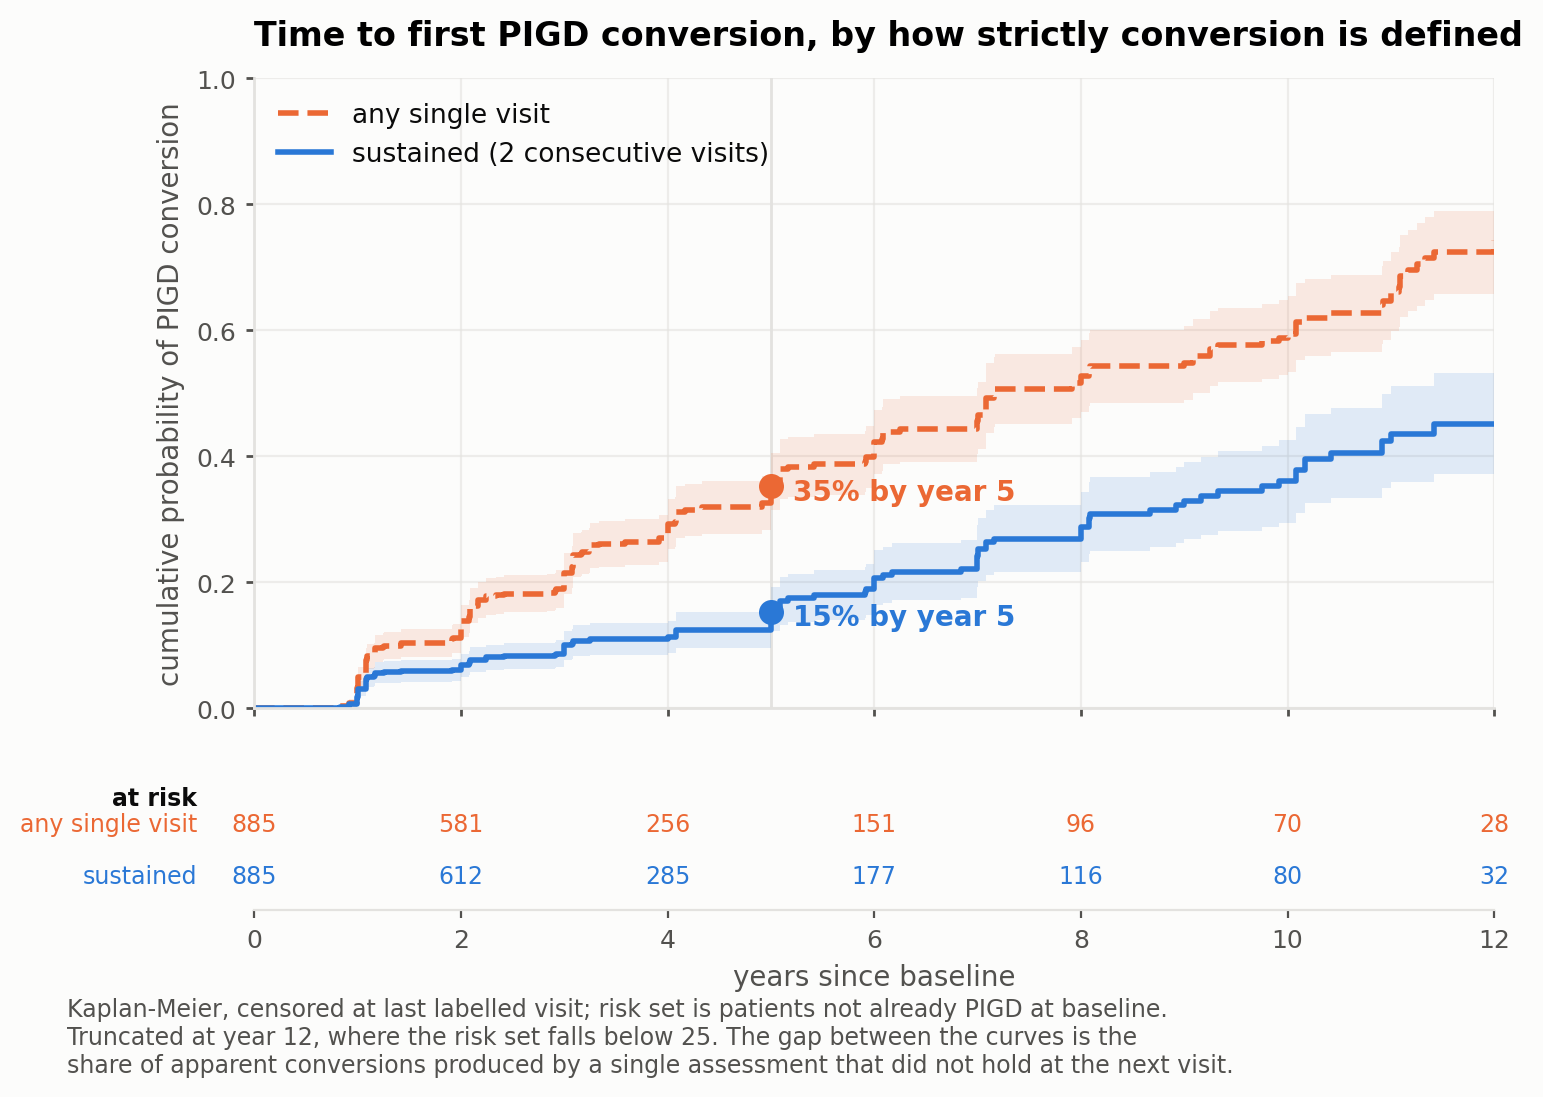
\includegraphics[width=0.78\textwidth]{f05_conversion.png}
\caption{Kaplan--Meier cumulative incidence of conversion to PIGD among the 885
patients not PIGD at their first labelled visit, under two definitions of the
event. Requiring the change to hold across two consecutive labelled visits more
than halves the five-year estimate, from 35.3\% to 15.3\%, on the same patients.}
\label{fig:conversion}
\end{figure}

\paragraph{Transition probabilities scale with the elapsed interval.}
TD$\to$TD fell from 0.820 at intervals of 1.5 years or less to 0.578 beyond four
years, while TD$\to$PIGD rose from 0.100 to 0.289
(Figure~\ref{fig:instability}c), the two interval-stratified intervals being
non-overlapping. A single pooled matrix therefore averages one-year and
multi-year transitions in whatever proportion attendance happened to produce, and
is not a property of the disease. This motivates the interval-aware
specifications of~\eqref{eq:ctmc} and~\eqref{eq:forward}.

\paragraph{The observed label is not first-order Markov.}
Testing whether the next label is conditionally independent of the previous one
given the current one rejects independence in all three current states
(Table~\ref{tab:dynamics}d): for current TD, $\chi^2 = 156.59$ on 4 degrees of
freedom over 1,583 triples ($P = 7.9 \times 10^{-33}$); for current
Indeterminate, $\chi^2 = 15.28$ over 235 triples ($P = 0.0042$); for current
PIGD, $\chi^2 = 61.15$ over 609 triples ($P = 1.7 \times 10^{-12}$). Concretely,
among currently-TD patients the probability of a PIGD outcome was 0.086 if the
previous label had been TD and 0.393 if it had been PIGD.

The correct reading is that the current recorded label is not a sufficient
statistic for the past. This motivates a latent-state formulation, in which a
slower underlying state carries the history the recorded label does not, but it
does not by itself establish one: unequal visit intervals and within-patient
correlation could also produce history dependence, and the test treats triples as
independent when patients contribute several.

\paragraph{The Indeterminate class behaves as a transient, but a pre-registered
test of that reading is inconclusive.}
A pre-registered audit compared the reversion rate after an \emph{entry} into
Indeterminate with that after a \emph{direct} TD--PIGD change
(Table~\ref{tab:dynamics}e). Entries revert at 0.543 (0.471--0.615) against 0.349
(0.298--0.397) for direct changes, a contrast of $+0.194$ ($+0.108$ to
$+0.281$); only 17.6\% of entries are sustained at the next visit, and 3 of 135
entries with two later visits are still Indeterminate at both. The median
Kaplan--Meier time to leave the Indeterminate label is 1.08 years, against 2.08
for PIGD and 5.41 for TD (Supplementary Figure~\ref{sfig:exit}). However, the
pre-registered reading rule also required the within-patient clustering of
Indeterminate visits to exceed what their frequency implies, and the
observed-to-expected ratio is 1.179 (0.988--1.391), which includes one. By its
own rule the audit is therefore \textbf{inconclusive}: the reversion contrast is
consistent with transient boundary crossing, but the clustering test does not
confirm it, and the statistic has low power at 441 visits.

\paragraph{Residual fluctuation is not pure measurement noise.}
Consecutive residual changes from a patient's own linear trend are negatively
correlated at lag 1 ($-0.219$, $-0.273$ to $-0.162$), but \emph{less} negatively
than independent noise with the same visit pattern implies ($-0.333$, $-0.369$ to
$-0.295$); the difference is $+0.113$ ($+0.046$ to $+0.179$, one-sided Monte
Carlo $P = 5\times10^{-4}$; Table~\ref{tab:dynamics}f). Part of a patient's
deviation from their own trend therefore persists to the next visit. This
indicates a state-space form, in which an unobserved level accumulates process
noise and is read with error, over an independent-noise growth form --- the
family to which the hidden Markov model and the nine-domain profile belong.

\begin{table}[t]
\centering
\caption{The dynamics of the recorded label, measured without fitting a
predictive model. All intervals are patient-clustered bootstraps unless stated.
Panel (e) is a pre-registered audit whose reading rule required both the
reversion contrast and the clustering statistic to agree; they do not, so the
audit is inconclusive by its own rule.}
\label{tab:dynamics}
\footnotesize
\begin{tabular}{@{}llll@{}}
\toprule
Quantity & Estimate & 95\% interval & Basis \\
\midrule
\multicolumn{4}{@{}l}{\textit{(a) Immediate reversion of an observed change (673 changes)}}\\
All observed changes            & 0.352 & (0.318, 0.388) & patient bootstrap \\
\quad TD $\to$ Indeterminate    & 0.560 & (0.478, 0.642) & patient bootstrap \\
\quad PIGD $\to$ Indeterminate  & 0.500 & (0.362, 0.648) & patient bootstrap \\
\quad TD $\to$ PIGD             & 0.320 & (0.253, 0.388) & patient bootstrap \\
\quad PIGD $\to$ TD             & 0.393 & (0.305, 0.481) & patient bootstrap \\
\addlinespace[3pt]
\multicolumn{4}{@{}l}{\textit{(b) Conversion to PIGD under two definitions (885 patients at risk)}}\\
Converted, single assessment    & 263 & --- & count \\
Converted, two consecutive      & 127 & --- & count \\
Reduction under the sustained rule & 0.517 & (0.457, 0.577) & patient bootstrap \\
Cumulative incidence at 5 y, single & 0.353 & (0.308, 0.399) & Kaplan--Meier \\
Cumulative incidence at 5 y, sustained & 0.153 & (0.120, 0.190) & Kaplan--Meier \\
\addlinespace[3pt]
\multicolumn{4}{@{}l}{\textit{(c) Dependence on the elapsed interval}}\\
$\Pr(\TD \to \TD)$, $\Delta \leq 1.5$ y & 0.820 & --- & stratified count \\
$\Pr(\TD \to \TD)$, $\Delta > 4$ y      & 0.578 & --- & stratified count \\
$\Pr(\TD \to \PIGD)$, $\Delta \leq 1.5$ y & 0.100 & --- & stratified count \\
$\Pr(\TD \to \PIGD)$, $\Delta > 4$ y    & 0.289 & --- & stratified count \\
\addlinespace[3pt]
\multicolumn{4}{@{}l}{\textit{(d) First-order Markov property in the recorded label}}\\
Current TD ($n{=}1{,}583$ triples)   & $\chi^2 = 156.59$ & $P = 7.9\times10^{-33}$ & $\chi^2$, df $=4$ \\
Current Indeterminate ($n{=}235$)    & $\chi^2 = 15.28$  & $P = 0.0042$ & $\chi^2$, df $=4$ \\
Current PIGD ($n{=}609$)             & $\chi^2 = 61.15$  & $P = 1.7\times10^{-12}$ & $\chi^2$, df $=4$ \\
\addlinespace[3pt]
\multicolumn{4}{@{}l}{\textit{(e) Pre-registered Indeterminate audit (inconclusive by its own rule)}}\\
Reversion after entry, $R_E$    & 0.543 & (0.471, 0.615) & patient bootstrap \\
Reversion after a direct change, $R_D$ & 0.349 & (0.298, 0.397) & patient bootstrap \\
Contrast $R_E - R_D$            & 0.194 & (0.108, 0.281) & patient bootstrap \\
Indeterminate sustained at two later visits & 0.022 & (0.000, 0.050) & patient bootstrap \\
Within-patient clustering, O/E, Indeterminate & 1.179 & (0.988, 1.391) & patient bootstrap \\
\addlinespace[3pt]
\multicolumn{4}{@{}l}{\textit{(f) Lag-1 autocorrelation of within-patient residual change (397 patients, 2,050 pairs)}}\\
Observed                        & $-0.219$ & ($-0.273$, $-0.162$) & patient bootstrap \\
Independent-noise null          & $-0.333$ & ($-0.369$, $-0.295$) & Monte Carlo \\
Observed $-$ null               & $+0.113$ & ($+0.046$, $+0.179$) & combined resample \\
\bottomrule
\end{tabular}

\end{table}

\paragraph{What follows.} The target changes often, a third of the change is
undone at once, its estimated conversion rate halves under a sustained-change
definition, its transition structure depends on attendance, and it is not
first-order Markov. Each of these is a property of the endpoint, measurable
before any model, and each bounds what a model trained on it can achieve.

\subsection{A generative model of the ratio does not reproduce the label}
\label{sec:ppc}

If the Indeterminate class is a transient crossing of a noisy continuous
quantity, then a generative model of that quantity should reproduce the label
record. We tested this directly, under a pre-registered protocol with a
calibrated threshold and positive controls.

A hierarchical growth model of the ratio with Student-t slopes and residuals was
fitted on 821 patients and 3,528 ratio-defined visits in five whole-patient
folds. For each patient, 500 patient-conditional replicate label sequences were
simulated from the fitted model and five pre-registered statistics computed: the
Indeterminate share, the reversion rate after an entry, the reversion rate after
a direct change, their difference, and the within-patient clustering ratio. The
omnibus statistic was compared against a threshold $c$ derived from 500 synthetic
null cohorts.

The verdict is \textbf{not reproduced} (Table~\ref{tab:ppc}):
$T_{\mathrm{obs}} = 3.091$ against $c = 2.577$. Two statistics fail. The observed
Indeterminate share is 0.1029 against a replicate mean of 0.0648, and the direct
reversion rate is 0.3115 against 0.4356 --- the model generates too few
Indeterminate visits and expects direct TD--PIGD changes to revert far more often
than they do. The reversion after entry and the clustering ratio are reproduced.
The check has power: the strong positive control was detected in 100 of 100
cohorts (lower 95\% bound 0.964), and three null-like controls in 6, 7 and 5 of
100.

\begin{table}[t]
\centering
\caption{Pre-registered posterior-predictive check of the label's dynamics under a
hierarchical growth model of the ratio with Student-t slopes and residuals (821
patients, 3,528 ratio-defined visits, 500 patient-conditional replicates). The
$z$ scores are capped at the resolution of the replicate distribution.}
\label{tab:ppc}
\small
\begin{tabular}{@{}llrrrl@{}}
\toprule
 & Statistic & Observed & Replicate mean & $z$ & $p$ \\
\midrule
$S_1$ & Indeterminate share                 & 0.1029 & 0.0648 & $-3.091$ & 0.001 \\
$S_2$ & Reversion after entry, $R_E$        & 0.5796 & 0.5555 & $-0.495$ & 0.310 \\
$S_3$ & Direct reversion, $R_D$             & 0.3115 & 0.4356 & $+3.091$ & 0.999 \\
$S_4$ & $R_E - R_D$                         & 0.2681 & 0.1200 & $-3.091$ & 0.001 \\
$S_5$ & Within-patient clustering, O/E      & 1.0334 & 1.0770 & $+0.207$ & 0.582 \\
\midrule
\multicolumn{6}{@{}l}{Omnibus $T_{\mathrm{obs}} = 3.091$ against the pre-registered threshold $c = 2.577$:
\textbf{not reproduced}}\\
\multicolumn{6}{@{}l}{Power: strong positive control detected in 100 of 100 cohorts (lower 95\% bound 0.964);}\\
\multicolumn{6}{@{}l}{three null-like controls in 6, 7 and 5 of 100.}\\
\bottomrule
\end{tabular}

\end{table}

Diagnostics localise the misfit without attaching a verdict
(Figure~\ref{fig:ppc}). The excess of 183 Indeterminate visits over the
generator's expectation is not uniform across the PIGD item sum: it sits at sums
2 (50\% of the excess), 3 (24\%) and 4--5 (22\%), and at sum 1 the observed and
expected counts agree (70 against 71.8). The reason is the lattice: a band of
nominal width 0.25 captures 1.82 times its width in lattice points at the lowest
PIGD sums, and if it captured only its nominal width the Indeterminate share
would be about 0.068, two thirds of the way from the observed 0.103 to the
generator's 0.051.

The direct-reversion deficit is entirely direction-specific. TD-to-PIGD changes
revert at 0.253 (0.187--0.325) against a generator expectation of 0.469 --- 37
observed reversions against 83 expected --- whereas PIGD-to-TD changes revert at
0.398 against an expectation of 0.396 (Supplementary
Figure~\ref{sfig:direction}). The misfit is present, and larger, among the 585
patients with no excluded PIGD-zero visit, so the exclusion of
Section~\ref{sec:undefined} is weakened as its driver.

\begin{figure}[t]
\centering
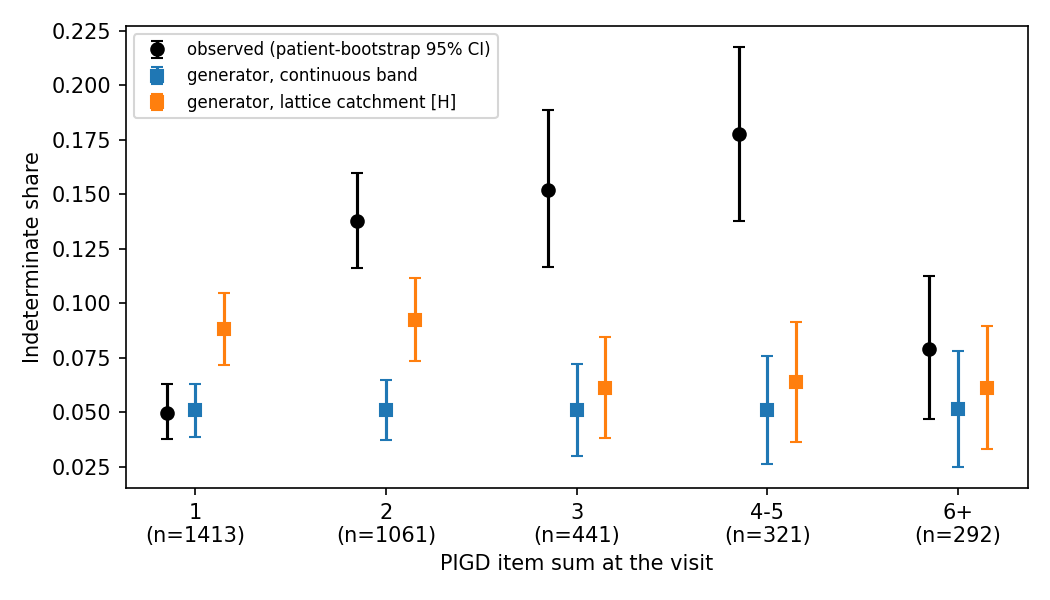
\includegraphics[width=0.84\textwidth]{f06_ppc.png}
\caption{Where the generative model of the ratio fails. Observed Indeterminate
share by PIGD item sum at the visit (black), against the expectation under the
fitted continuous-ratio generator treating the band as a continuous interval
(blue) and as the catchment of lattice points it actually contains (orange).
Intervals are patient-clustered bootstraps for the observed values and predictive
intervals for the generator. The excess is concentrated at PIGD item sums 2 to 5
and is largely explained by the lattice, not by an additional state.}
\label{fig:ppc}
\end{figure}

\paragraph{Interpretation.} A continuous-ratio growth model with heavy tails
cannot reproduce two features of the label record: the Indeterminate share, which
the integer lattice inflates inside the band, and the persistence of TD-to-PIGD
changes, which a symmetric-noise model under-predicts. Both are features of how
the label is constructed from integer item sums rather than of the patients.
Nothing here is evidence for or against a biological intermediate subtype. The
diagnostic recommendation was that a measurement-faithful integer-score model
with no intermediate state should be the next test; that model was specified but
never run on the cohort (Supplementary~\ref{sup:notrun}), so the question
remains open.

\subsection{Models of the label itself}
\label{sec:discrete}

Under leave-one-patient-out validation on the 3,361 transitions
(Table~\ref{tab:lopo}, Figure~\ref{fig:lopo}), the hidden Markov model reached
accuracy 0.7539 (95\% CI 0.7348--0.7731), the discrete-time chain 0.7474
(0.7272--0.7670), the continuous-time chain 0.7453 (0.7250--0.7646), the
persistence rule 0.7227 (0.7009--0.7437) and the marginal null 0.6293
(0.6011--0.6565). On the proper scores the ordering is the same and the
separation is larger: log-likelihood per prediction $-0.673$ for the hidden
Markov model against $-0.707$ and $-0.711$ for the chains, and three-class Brier
0.369 against 0.390 and 0.393.

\begin{table}[t]
\centering
\caption{Leave-one-patient-out three-class prediction of the next recorded label
(934 folds, 3,361 predictions). $^{\dagger}$The persistence rule emits only zero
and one, so its log-likelihood is degenerate and its Brier score reflects that.}
\label{tab:lopo}
\footnotesize
\setlength{\tabcolsep}{4pt}
\begin{tabular}{@{}lrlrrr@{}}
\toprule
Model & Accuracy & 95\% CI & Mean per-patient & Log-lik.\ / pred. & Brier \\
\midrule
Hidden Markov model, 3 latent states & 0.7539 & (0.7348, 0.7731) & 0.7538 & $-0.6726$ & 0.3688 \\
Markov chain, discrete-time          & 0.7474 & (0.7272, 0.7670) & 0.7513 & $-0.7066$ & 0.3896 \\
Markov chain, continuous-time        & 0.7453 & (0.7250, 0.7646) & 0.7481 & $-0.7105$ & 0.3925 \\
\textbf{Persistence} (recorded label)& \textbf{0.7227} & (0.7009, 0.7437) & 0.7213 & $-7.662^{\dagger}$ & 0.5546 \\
Marginal null                        & 0.6293 & (0.6011, 0.6565) & 0.6404 & $-0.8756$ & 0.5211 \\
\midrule
\multicolumn{6}{@{}l}{\textit{Per-class performance of the hidden Markov model}}\\
\multicolumn{2}{@{}l}{Class} & Support & Predicted & Recall & Precision \\
\multicolumn{2}{@{}l}{TD}            & 2,115 & 2,450 & 0.9102 & 0.7857 \\
\multicolumn{2}{@{}l}{Indeterminate} & 332   & \textbf{1} & \textbf{0.0000} & --- \\
\multicolumn{2}{@{}l}{PIGD}          & 914   & 910   & 0.6663 & 0.6692 \\
\midrule
\multicolumn{6}{@{}l}{\textit{Accuracy by the label recorded at the prediction point}}\\
\multicolumn{2}{@{}l}{Current TD ($n{=}2{,}261$)} & \multicolumn{4}{l}{0.8107} \\
\multicolumn{2}{@{}l}{Current Indeterminate ($n{=}334$)} & \multicolumn{4}{l}{0.4880} \\
\multicolumn{2}{@{}l}{Current PIGD ($n{=}766$)} & \multicolumn{4}{l}{0.7023} \\
\bottomrule
\end{tabular}

\end{table}

\begin{figure}[t]
\centering
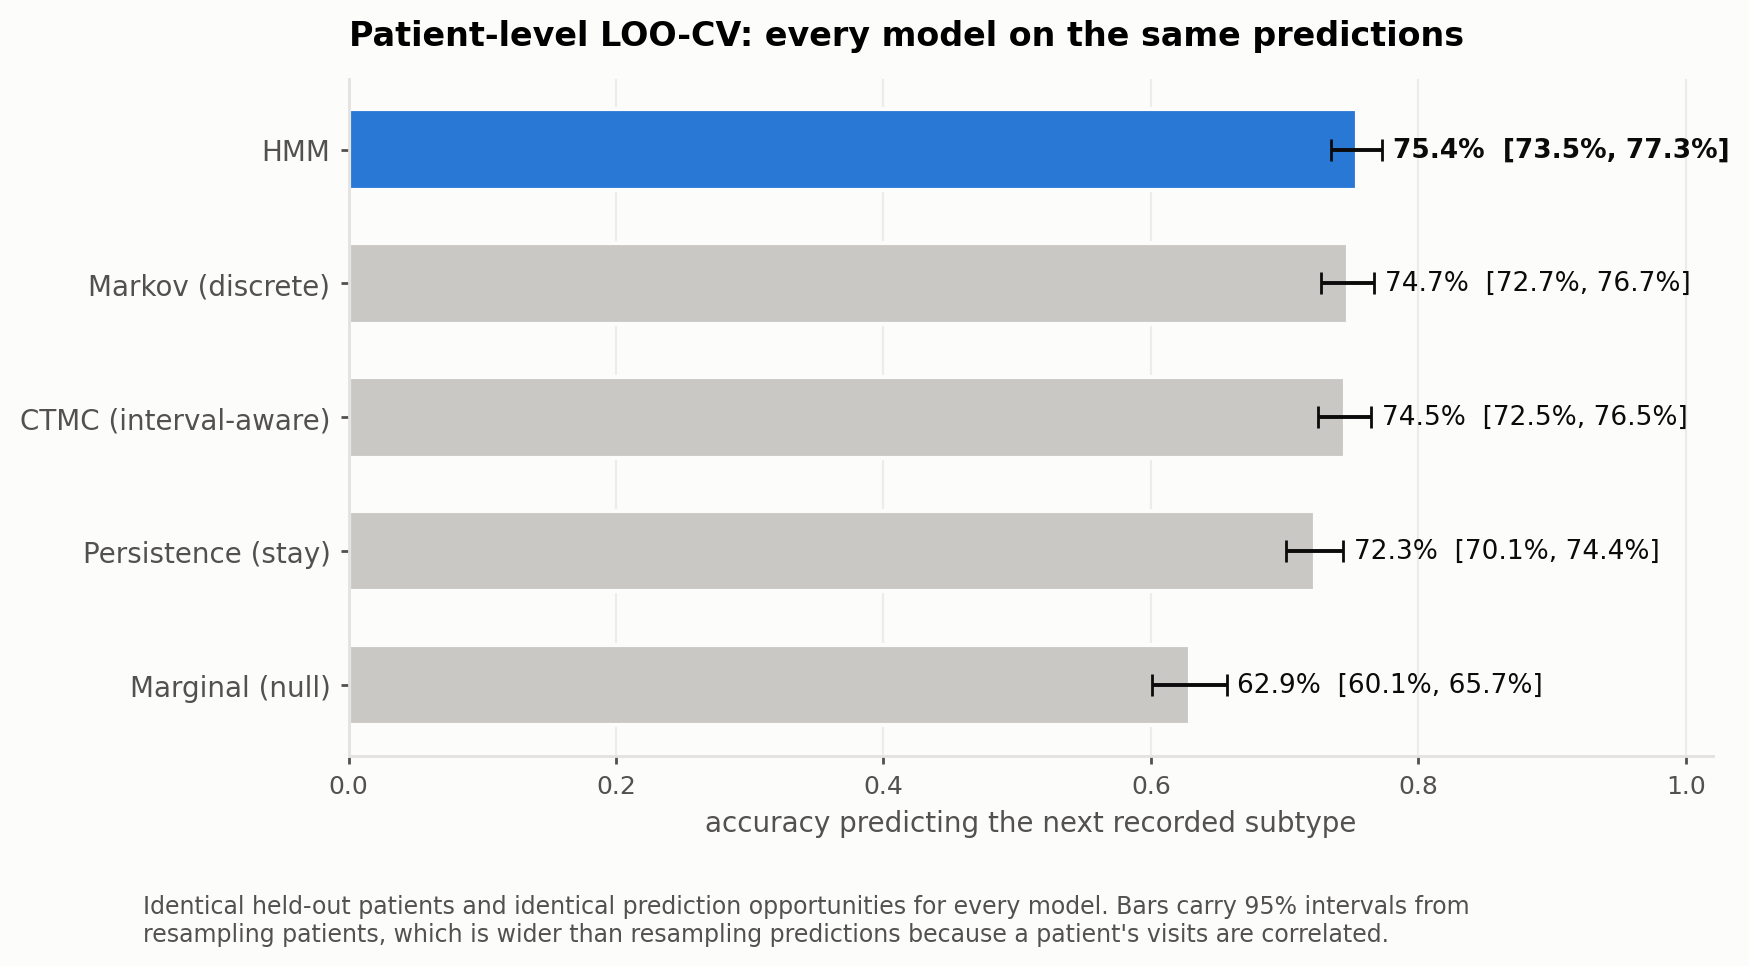
\includegraphics[width=0.84\textwidth]{f08_lopo.png}
\caption{Leave-one-patient-out three-class comparison of the hidden Markov model,
the two observed-label chains, the persistence rule and the marginal null on the
same 3,361 transitions.}
\label{fig:lopo}
\end{figure}

Three features of this result matter more than the ordering.

\paragraph{The margin over the trivial rule is three points.} The hidden Markov
model's advantage over persistence is $+3.1$ accuracy points (95\% CI $+2.2$ to
$+4.1$, from the harmonised contrast of Section~\ref{sec:harmonised}); its
advantage over the discrete chain is 0.7 points. The latent layer is nonetheless
strongly supported on information criteria against the best alternative on a
common joint likelihood ($\Delta$AIC 224, $\Delta$BIC 186;
Supplementary~\ref{sup:misc}), and on a single 70/30 split it beat the discrete
chain in 10 of 10 resamples by $+0.028$ log-likelihood per pair
(Supplementary~\ref{sup:hmm}). The latent layer earns its parameters on the
probabilities; it barely moves the thresholded call.

\paragraph{The model never predicts the Indeterminate class.} It issues that
label \textbf{once in 3,361 predictions} (recall 0.000), because the
Indeterminate probability never exceeds the TD or PIGD probability under the
argmax rule --- its maximum over the whole evaluation set is 0.371. This is the
correct consequence of the label's own dynamics: an Indeterminate visit is
followed by Indeterminate only 19\% of the time. The fitted misclassification
matrix records the same fact in its parameters (Figure~\ref{fig:emission}): the
latent TD state is recorded correctly at 0.941 and the latent PIGD state at
0.842, while the latent Indeterminate row sits exactly at the constraint floor of
0.500. The data do not identify an Indeterminate state that is recorded as
Indeterminate more than half the time.

\begin{figure}[t]
\centering
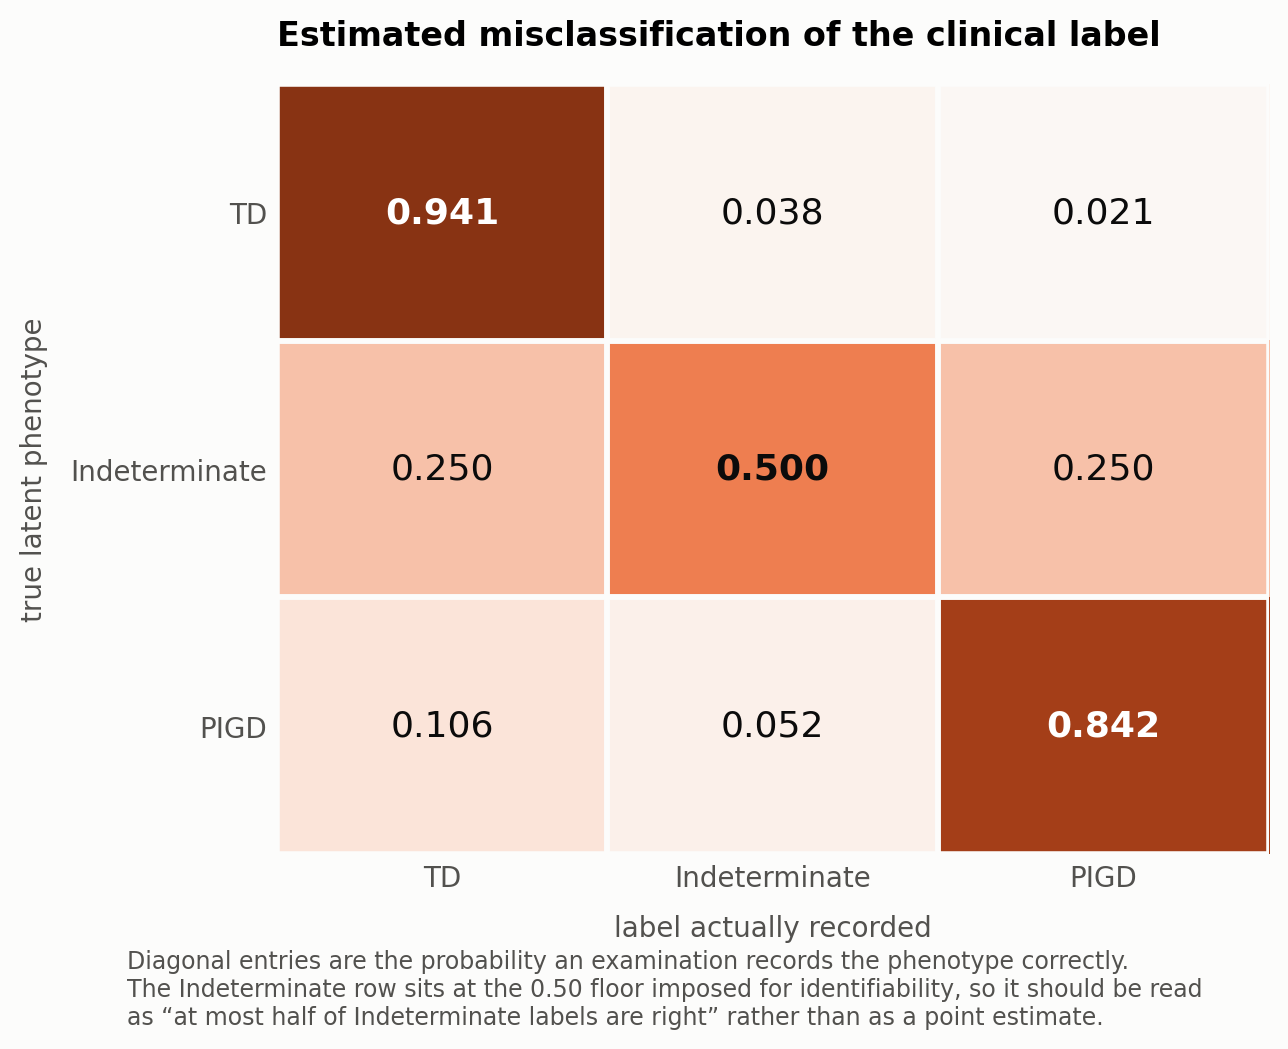
\includegraphics[width=0.60\textwidth]{f07_emission.png}
\caption{Fitted misclassification matrix $E$ of the three-state hidden Markov
model: rows are latent states, columns the probability of each recorded label.
The latent Indeterminate row sits exactly at the imposed floor of 0.5, which is a
result about that state rather than an artefact of the constraint.}
\label{fig:emission}
\end{figure}

\paragraph{Neither more latent states nor fewer constraints change the picture.}
A five-state specification scored 0.7513, below the three-state model, and
reported convergence in only 404 of 934 folds (43.3\%) against 934 of 934 for
every other specification, so 59.2\% of its predictions come from non-converged
fits; it is reported as a negative result about capacity and not used further.
Removing the emission floor, or fitting four or five states without it, changes
held-out accuracy by at most 0.002 (Supplementary~\ref{sup:hmm}). The
three-state floor-constrained fit has a unique optimum --- all 40 random starts
reach the same log-likelihood to within 0.01 --- whereas the unconstrained
three-state fit sits on a ridge and the five-state fit is multimodal (1 of 40
starts within 0.01 of the best). A prior-corrected decision rule that divides each
predicted probability by its class prevalence recovers Indeterminate recall of
0.25 to 0.32 at the cost of accuracy, which falls to 0.68--0.71; the probabilities
themselves do not change, which locates the failure in the decision rule's
interaction with a rare class rather than in the fitted model.

\subsection{Models of the continuous quantity the label is cut from}
\label{sec:continuous}

\subsubsection{The hierarchical Bayesian growth model}

Fitted on 2,426 ratio observations from 573 training patients, the growth model
estimates a \textbf{population trend of $-0.0927$ per year} in the ratio, with a
95\% credible interval of $-0.1159$ to $-0.0682$ (Table~\ref{tab:growth},
Figure~\ref{fig:growth}). The posterior probability that the population slope is
negative is 1.000. On the clinical scale this is a slow drift of the cohort
average away from tremor dominance and towards PIGD.

\begin{table}[t]
\centering
\caption{Hierarchical Bayesian growth model of the ratio~\eqref{eq:hb}: posterior
summary, the relationship between the residual spread and the Indeterminate band,
and the head-to-head comparison with the hidden Markov model on the transitions
both can score. Intervals are 95\% credible intervals.}
\label{tab:growth}
\small
\begin{tabular}{@{}llrl@{}}
\toprule
Parameter & Interpretation & Mean & 95\% CrI \\
\midrule
$\beta_0$ & population baseline ratio              & 2.2920 & (2.1577, 2.4272) \\
$\beta_1$ & population change in $r$, per year     & $-0.0927$ & ($-0.1159$, $-0.0682$) \\
$\sigma$  & total residual SD                      & 1.1380 & (1.0993, 1.1778) \\
$\tau_0$  & between-patient SD of intercepts       & 1.3408 & (1.2466, 1.4421) \\
$\tau_1$  & between-patient SD of slopes, per year & 0.1033 & (0.0780, 0.1315) \\
\midrule
\multicolumn{4}{@{}l}{\textit{Residual spread against the width of the Indeterminate band}}\\
\multicolumn{2}{@{}l}{$\sigma$ / band width ($0.25$)} & \multicolumn{2}{l}{4.6} \\
\multicolumn{2}{@{}l}{Variance of $r$: between / within patients} & \multicolumn{2}{l}{53.6\% / 46.4\%} \\
\midrule
\multicolumn{4}{@{}l}{\textit{Head to head against the hidden Markov model on the 825 pairs both can score}}\\
\multicolumn{2}{@{}l}{Hidden Markov model} & \multicolumn{2}{l}{log-lik.\ $-0.6559$; accuracy 0.7612; Brier 0.3573} \\
\multicolumn{2}{@{}l}{Hierarchical Bayesian growth} & \multicolumn{2}{l}{log-lik.\ $-0.6814$; accuracy 0.7370; Brier 0.3786} \\
\multicolumn{2}{@{}l}{Across six further patient splits} & \multicolumn{2}{l}{HMM ahead 6 of 6, mean $+0.0579$ (SD 0.0188)} \\
\bottomrule
\end{tabular}

\end{table}

\begin{figure}[t]
\centering
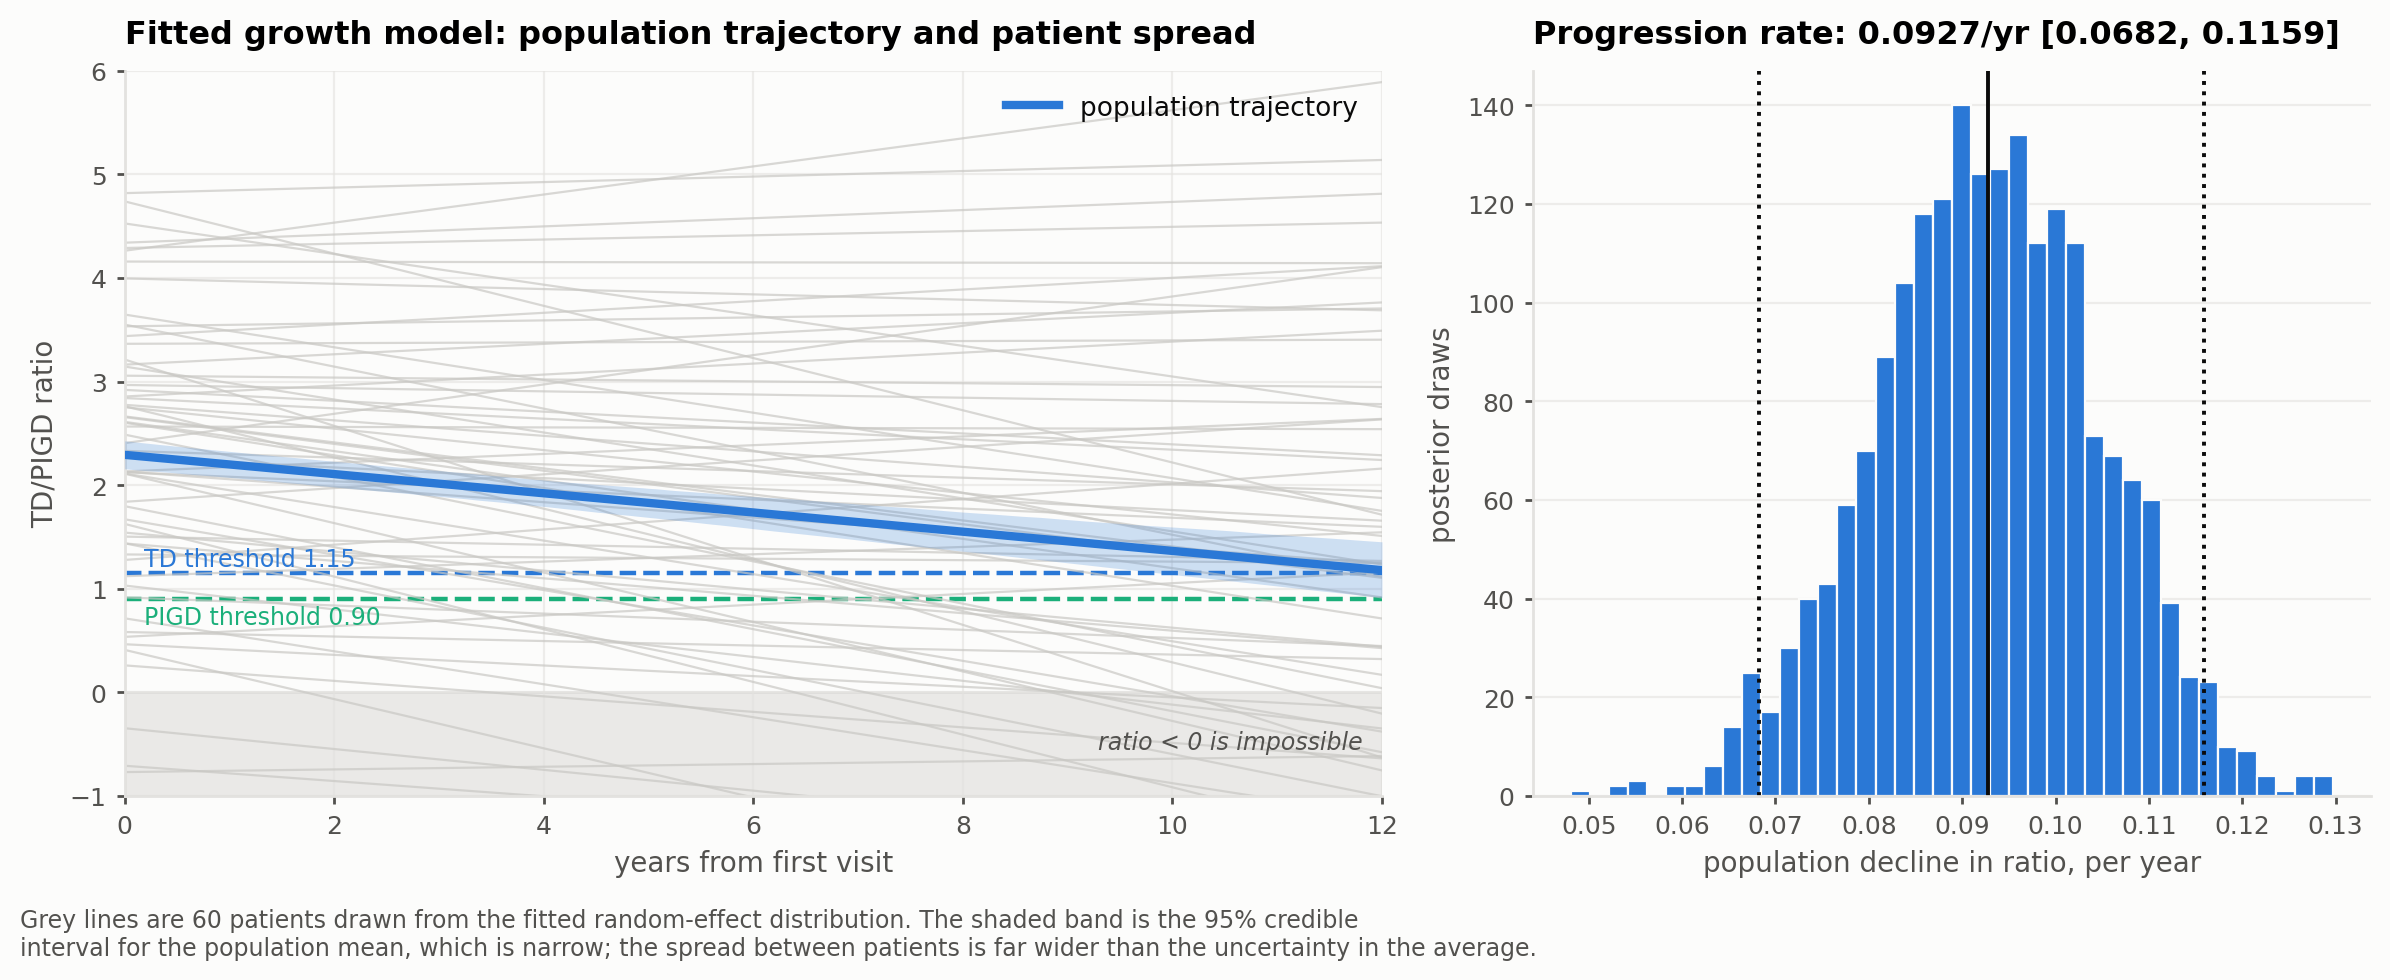
\includegraphics[width=\textwidth]{f09_growth.png}
\caption{Hierarchical Bayesian growth model of the ratio. \textbf{Left:} the
fitted population trajectory (heavy line) with its 95\% credible band, against 60
patient trajectories drawn from the fitted random-effect distribution (grey); the
two classification thresholds are marked. The credible band on the population
mean is narrow while the spread between patients is wide, so the population trend
is not a patient-level progression rate. The shaded region below zero marks ratio
values that cannot occur, on which the Gaussian likelihood nonetheless places
mass. \textbf{Right:} the posterior for the population rate of decline.}
\label{fig:growth}
\end{figure}

Three features of the posterior matter more than the trend itself.

First, \textbf{the population trend is not a patient-level progression rate}. The
between-patient SD of slopes is $\tau_1 = 0.103$ per year, comparable in
magnitude to the population slope of $-0.093$ itself, so the fitted distribution
of individual slopes spans both signs. The credible interval in
Table~\ref{tab:growth} is an interval on the \emph{cohort average}, and
Figure~\ref{fig:growth} shows how much wider the spread of individual
trajectories is than the uncertainty in that average. A statement about the
population here licenses no statement about an individual patient. The ratio's
variance decomposes into 53.6\% between patients and 46.4\% within them.

Second, \textbf{the residual spread dwarfs the Indeterminate band}. The total
residual SD is $\sigma = 1.138$ (1.099--1.178) against a band 0.25 wide --- a
factor of \textbf{4.6}. A model predicting which of three bands the next ratio
falls in must place a predictive distribution several times wider than the middle
band, so under an argmax decision rule the middle class is almost never the most
probable outcome. The failure of every family to recover the Indeterminate class
is in this sense a consequence of the representation rather than of any model's
capacity.

Third, on prediction of the next recorded label the growth model does not improve
on the latent-state model. Compared on the same 825 held-out transitions both can
score, the hidden Markov model reached a held-out log-likelihood of $-0.656$ per
transition against the growth model's $-0.681$, with accuracies of 0.761 and
0.737 and Brier scores of 0.357 and 0.379; across six further patient-level
splits the hidden Markov model was ahead in 6 of 6, by a mean of $+0.058$ (SD
0.019; paired $t$-test $P = 6.6\times10^{-4}$, Wilcoxon $P = 0.031$). The growth
model under-predicts PIGD in every reliability bin, with a mean gap of 0.105,
which is what a Gaussian on a quantity this dispersed does near a threshold.

Student-t variants resolve one question and close another. Heavy-tailed
\emph{residuals} improve held-out prediction unambiguously ($+0.112$ log
predictive density per visit, $+0.061$ to $+0.168$, positive in 7 of 7 splits;
residual degrees of freedom about 2.1). Heavy-tailed \emph{slopes} are
\textbf{not supported}: a pre-registered reassessment with a converged sampler met
the per-split criterion in only 1 of 7 splits against a threshold of 5, with zero
false flags in 180 null calibration cohorts and 55 of 60 detections in the
positive control (Supplementary~\ref{sup:studentt}). The heavy residual tails are
the same phenomenon the lag-1 and posterior-predictive analyses see: occasional
large excursions of the ratio that do not persist.

\subsubsection{Gaussian processes on the ratio and on the subscores}

\paragraph{On the ratio, a flexible kernel helps.}
On one-step-ahead prediction of the ratio (821 patients, 2,707 held-out points),
the squared-exponential kernel $K_1$ reached a pooled MAE of 0.972 against 1.005
for the linear-trend kernel $K_0$ (Table~\ref{tab:gp}, Figure~\ref{fig:gpr}). The
paired difference is \textbf{$-0.033$ (95\% CI $-0.047$ to $-0.021$)}, and the
same sign and significance hold when errors are averaged within patients before
pooling ($-0.019$, $-0.028$ to $-0.011$). Departures from a straight line
therefore carry predictive signal on this quantity, and the Gaussian process also
beats persistence on the ratio by $-0.071$ ($-0.098$ to $-0.045$).

The remaining kernel contrasts were inconclusive or null. Adding a linear term
beside an RBF changed MAE by about $10^{-6}$, and its variance pinned at its lower
bound in every fold; a Matérn-3/2 kernel did not improve on the squared
exponential ($-0.0005$, $-0.0015$ to $+0.0005$). The linear-kernel Gaussian
process and the hierarchical Bayesian growth model --- two different
implementations of the same linear-trend assumption --- were also
indistinguishable ($-0.0009$, $-0.0033$ to $+0.0014$), which is an internal
consistency check rather than a finding.

\begin{table}[t]
\centering
\caption{Gaussian process results. (\textbf{a}) One-step-ahead prediction of the
ratio. (\textbf{b}) Paired kernel and baseline contrasts on the ratio; negative
values favour the first-named specification, since the metric is MAE.
(\textbf{c}) The two subscores modelled separately on the full evaluation set.
All intervals are patient-clustered bootstraps.}
\label{tab:gp}
\small
\setlength{\tabcolsep}{5pt}
\begin{tabular}{@{}llrrrr@{}}
\toprule
Target & Specification & MAE & RMSE & CRPS & Cov.\ 95\% \\
\midrule
\multicolumn{6}{@{}l}{\textit{(a) Ratio $r$; 821 patients, 2,707 held-out points}}\\
 & GP, linear kernel ($K_0$)            & 1.005 & 1.387 & 0.747 & 0.939 \\
 & GP, RBF kernel ($K_1$)               & \textbf{0.972} & 1.357 & 0.725 & 0.941 \\
 & GP, linear $+$ RBF ($K_2$)           & 0.972 & 1.357 & 0.725 & 0.941 \\
 & GP, linear $+$ Mat\'ern-3/2 ($K_3$)  & 0.971 & 1.356 & 0.725 & 0.941 \\
 & Hierarchical Bayesian growth model   & 1.006 & 1.391 & 0.748 & 0.930 \\
 & Persistence                          & 1.043 & 1.540 & 0.818 & 0.936 \\
 & Patient mean                         & 1.063 & 1.471 & 0.800 & 0.941 \\
 & Population mean                      & 1.395 & 1.801 & 0.984 & 0.948 \\
\addlinespace[4pt]
\multicolumn{6}{@{}l}{\textit{(b) Paired contrasts on the ratio (MAE; negative favours the first-named)}}\\
\multicolumn{2}{@{}l}{$K_1 - K_0$: does a flexible kernel beat a linear trend?}
   & \multicolumn{4}{l}{$-0.0333$ \,($-0.0467$, $-0.0205$)\quad \textbf{favours $K_1$}} \\
\multicolumn{2}{@{}l}{$K_3 - K_1$: does Mat\'ern beat squared exponential?}
   & \multicolumn{4}{l}{$-0.0005$ \,($-0.0015$, $+0.0005$)\quad inconclusive} \\
\multicolumn{2}{@{}l}{$K_0 - $ growth model: do the two linear forms agree?}
   & \multicolumn{4}{l}{$-0.0009$ \,($-0.0033$, $+0.0014$)\quad inconclusive} \\
\multicolumn{2}{@{}l}{$K_1 - $ persistence}
   & \multicolumn{4}{l}{$-0.0707$ \,($-0.0979$, $-0.0451$)\quad \textbf{favours $K_1$}} \\
\addlinespace[4pt]
\multicolumn{6}{@{}l}{\textit{(c) Subscores modelled separately; 934 patients, 3,361 held-out points}}\\
 & Tremor: GP ($K_1$)                   & 0.2395 & --- & 0.1708 & 0.936 \\
 & Tremor: persistence                  & 0.2426 & --- & 0.1797 & 0.953 \\
 & PIGD: GP ($K_1$)                     & 0.2175 & --- & 0.1618 & 0.933 \\
 & PIGD: persistence                    & \textbf{0.2040} & --- & 0.1724 & 0.951 \\
\addlinespace[2pt]
\multicolumn{2}{@{}l}{Tremor: GP $-$ persistence (MAE)}
   & \multicolumn{4}{l}{$-0.0031$ \,($-0.0084$, $+0.0022$)\quad inconclusive} \\
\multicolumn{2}{@{}l}{PIGD: GP $-$ persistence (MAE)}
   & \multicolumn{4}{l}{$+0.0134$ \,($+0.0083$, $+0.0187$)\quad \textbf{favours persistence}} \\
\multicolumn{2}{@{}l}{Joint (tremor $+$ PIGD): GP $-$ persistence (log score)}
   & \multicolumn{4}{l}{$+0.1437$ \,($+0.1020$, $+0.1860$)\quad \textbf{favours the GP}} \\
\bottomrule
\end{tabular}

\end{table}

\begin{figure}[t]
\centering
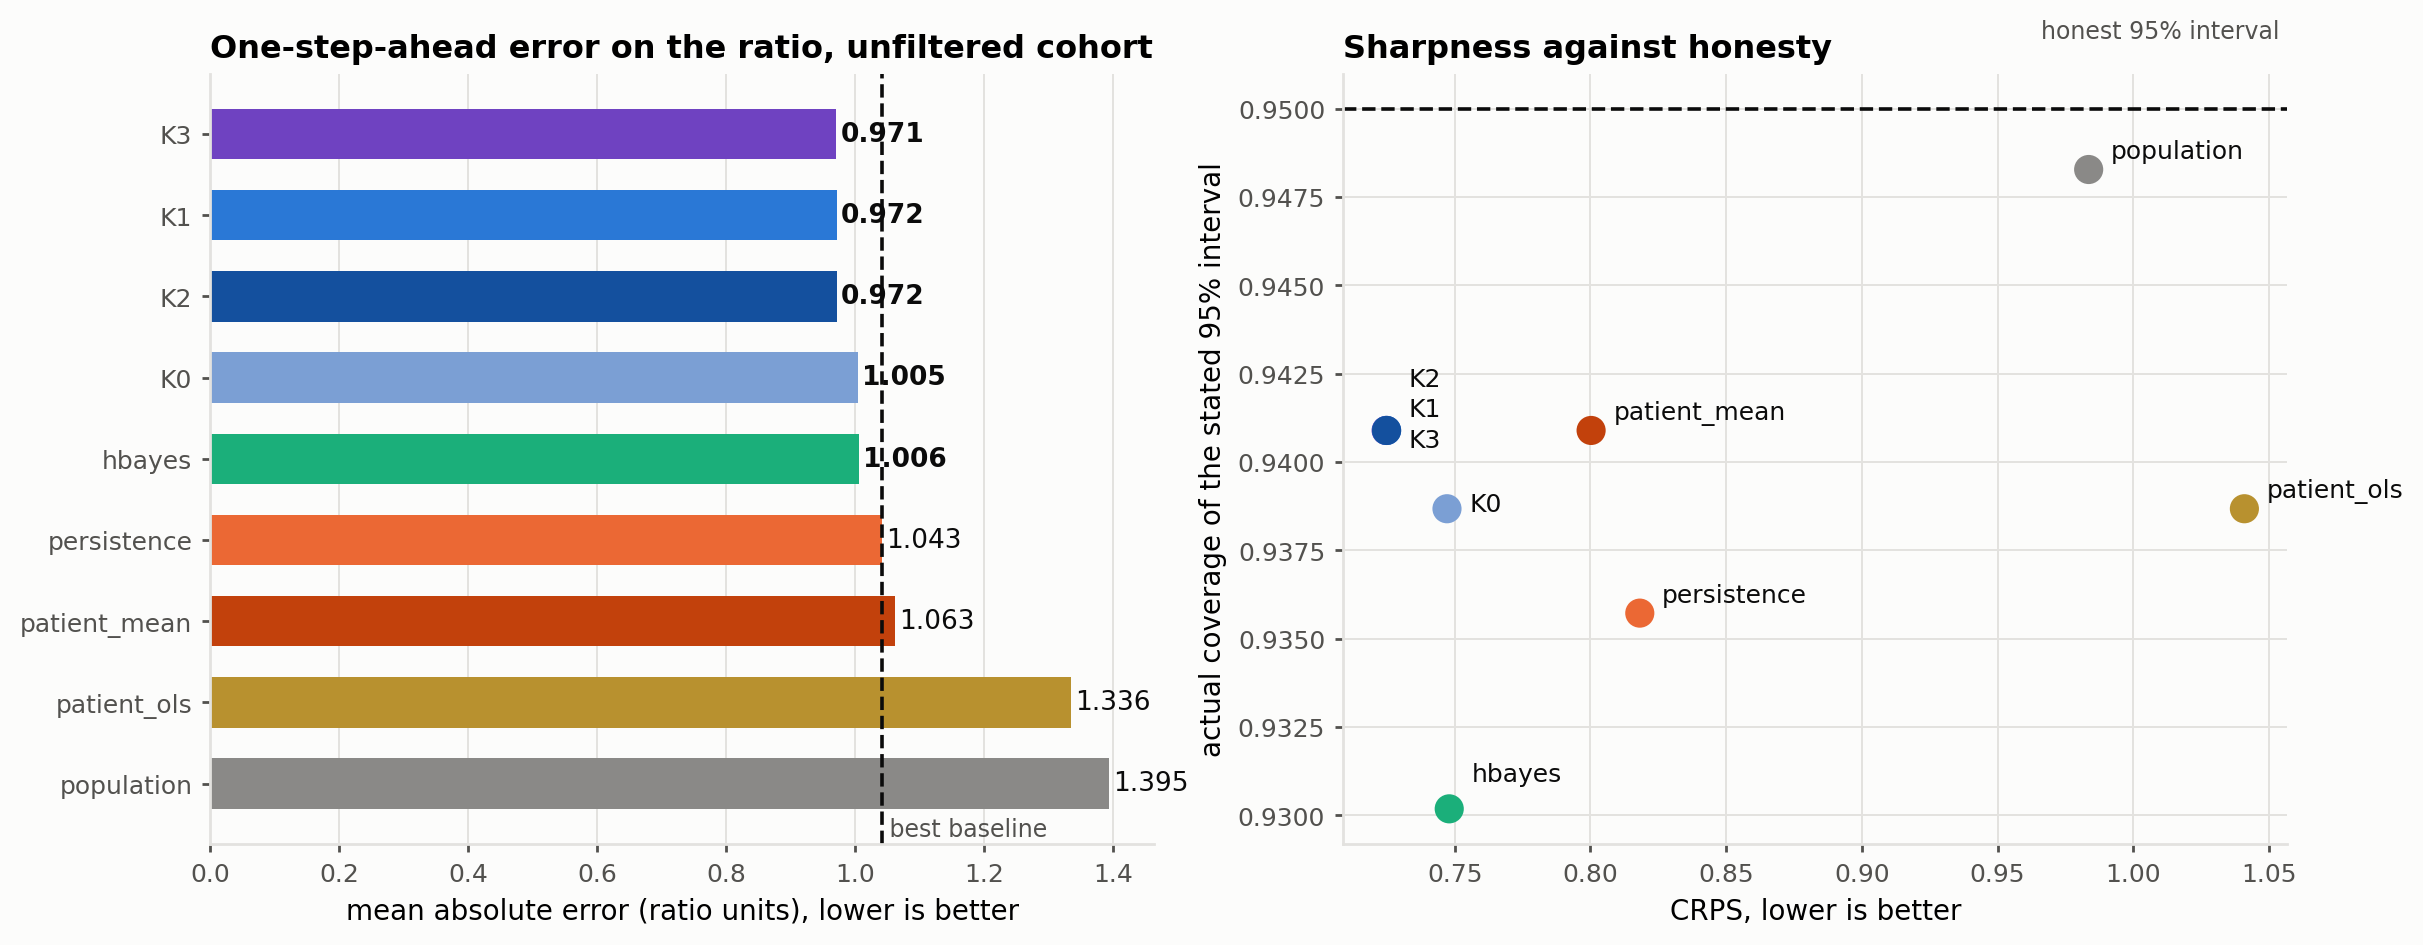
\includegraphics[width=\textwidth]{f10_gpr.png}
\caption{Gaussian process regression on the ratio, one step ahead and
leave-one-patient-out on 2,707 held-out points. \textbf{Left:} mean absolute
error in ratio units, lower being better, for the four kernels of
Section~\ref{sec:gp}, the hierarchical Bayesian growth model and the rule
baselines; the dashed line marks the best baseline. The RBF kernels separate from
the linear kernel $K_0$ and from the growth model, which are themselves
indistinguishable. \textbf{Right:} CRPS against the realised coverage of the
stated 95\% predictive interval, with nominal coverage marked. All specifications
are slightly under-covered.}
\label{fig:gpr}
\end{figure}

\paragraph{On the subscores, it does not.}
The advantage does not survive the change of target. Modelled separately on the
full evaluation set of 3,361 points from 934 patients --- which recovers the 654
points and 113 patients the ratio model cannot score --- the Gaussian process
\textbf{did not beat persistence on the tremor subscore} ($-0.0031$, 95\% CI
$-0.0084$ to $+0.0022$) and was \textbf{worse than persistence on the PIGD
subscore} ($+0.0134$, 95\% CI $+0.0083$ to $+0.0187$, in favour of the trivial
rule). The jointly-covarying form changed nothing: the full coregionalisation
block differs from its diagonal counterpart by $-0.0003$ on tremor and $-0.0001$
on PIGD, both intervals containing zero, because the two subscores are nearly
uncorrelated (random-intercept correlation $-0.015$, residual correlation
$+0.019$).

The reason is the point mass at zero. At the 446 held-out visits where the PIGD
subscore is zero, persistence predicts below 0.1 at 62\% of them while the
Gaussian process never does --- its mean prediction there is 0.242. A continuous
Gaussian model cannot reproduce an exact zero, and a sixth of this cohort's visits
carry one. The same misspecification is visible as predictive mass below zero:
12.9\% to 13.9\% of each ratio predictive distribution and 5.3\% of the tremor
distribution fall on values the quantity cannot take.

On proper scores the picture reverses: every Gaussian process beats persistence
on CRPS and log score for both subscores (joint log score $+0.144$, $+0.102$ to
$+0.186$), and kernels with both a linear and a flexible component beat the
simpler ones ($K_2 - K_0$ joint log score $+0.073$, $+0.051$ to $+0.096$). A
model can be better calibrated and simultaneously worse on absolute error when the
target has an atom the model cannot represent.

\paragraph{Deriving the label from the subscores.}
Pushed through the unchanged rule~\eqref{eq:rule} by Monte Carlo, the independent
subscore Gaussian process reaches three-class accuracy 0.7566 against the hidden
Markov model's 0.7539 \emph{on exactly the same 934 patients and 3,361 points},
a paired difference of \textbf{$+0.27$ accuracy points (95\% CI $-0.42$ to
$+0.98$)}. The interval contains zero. The jointly-covarying form gives $+0.45$
points ($-0.26$ to $+1.17$). On log loss the Gaussian processes are better than
the hidden Markov model ($-0.020$, $-0.032$ to $-0.007$) and the mixed model is
worse ($+0.018$, $+0.004$ to $+0.032$).

This is the first like-for-like comparison of the continuous route against the
categorical route in this programme, and its answer is that they are
indistinguishable on accuracy at this sample size. \textbf{That is a failure to
detect a difference, not a demonstration of equivalence}: the interval is roughly
1.4 accuracy points wide, no equivalence margin was pre-specified, and the two
models differ on quantities this comparison does not measure --- their probability
vectors, what else they predict, and what they require as input.

\paragraph{Time-varying rates are a population description, not a predictive
feature.} A linear-spline mixed model finds the PIGD slope rising across
follow-up (0.045, 0.057 and 0.080 per year in years 0--2, 2--5 and beyond 5) and
the tremor slope falling (0.033, 0.033 and 0.013), with the same pattern within
the 226 patients observed in both periods. A dedicated audit confirms a departure
from linearity (supremum likelihood ratio 39.1 against a bootstrap 95th
percentile of 7.7, $P = 0.005$) but finds \emph{no identifiable knot} (best
single knot 4.75 years, bootstrap range 2.5 to 10 years), Wald intervals on the
late-period slopes too narrow by factors of 1.7 and 2.2 against a patient
bootstrap, and informative attrition (log-odds of loss to follow-up rising by
$+0.52$ per point of PIGD score). On held-out prediction the spline improves PIGD
MAE by $-0.0034$ and tremor not at all, and both lose to persistence
(Supplementary~\ref{sup:temporal}).

\subsection{The harmonised comparison and where each margin lives}
\label{sec:harmonised}

Placing all fourteen specifications on one case list under one decision rule
(Table~\ref{tab:families}, Figure~\ref{fig:families}) gives the programme's
central result. The nine fitted specifications span \textbf{1.22 accuracy
points}, from 0.7453 to 0.7575. Every one exceeds the persistence rule by a
margin whose interval excludes zero, between $+0.0226$ (0.0135--0.0316) and
$+0.0348$ (0.0252--0.0450); and the intervals overlap heavily with each other,
the gap between the best and the worst fitted specification being smaller than
the width of any single interval.

The families differ in almost every modelling choice that is supposed to matter:
categorical against continuous observations, discrete against continuous time, a
memoryless chain against a latent state read through a misclassification matrix,
six parameters against several dozen, a parametric linear trend against a
non-parametric Gaussian process. None of those choices moves the accuracy at
which the next recorded label is reproduced.

\begin{figure}[t]
\centering
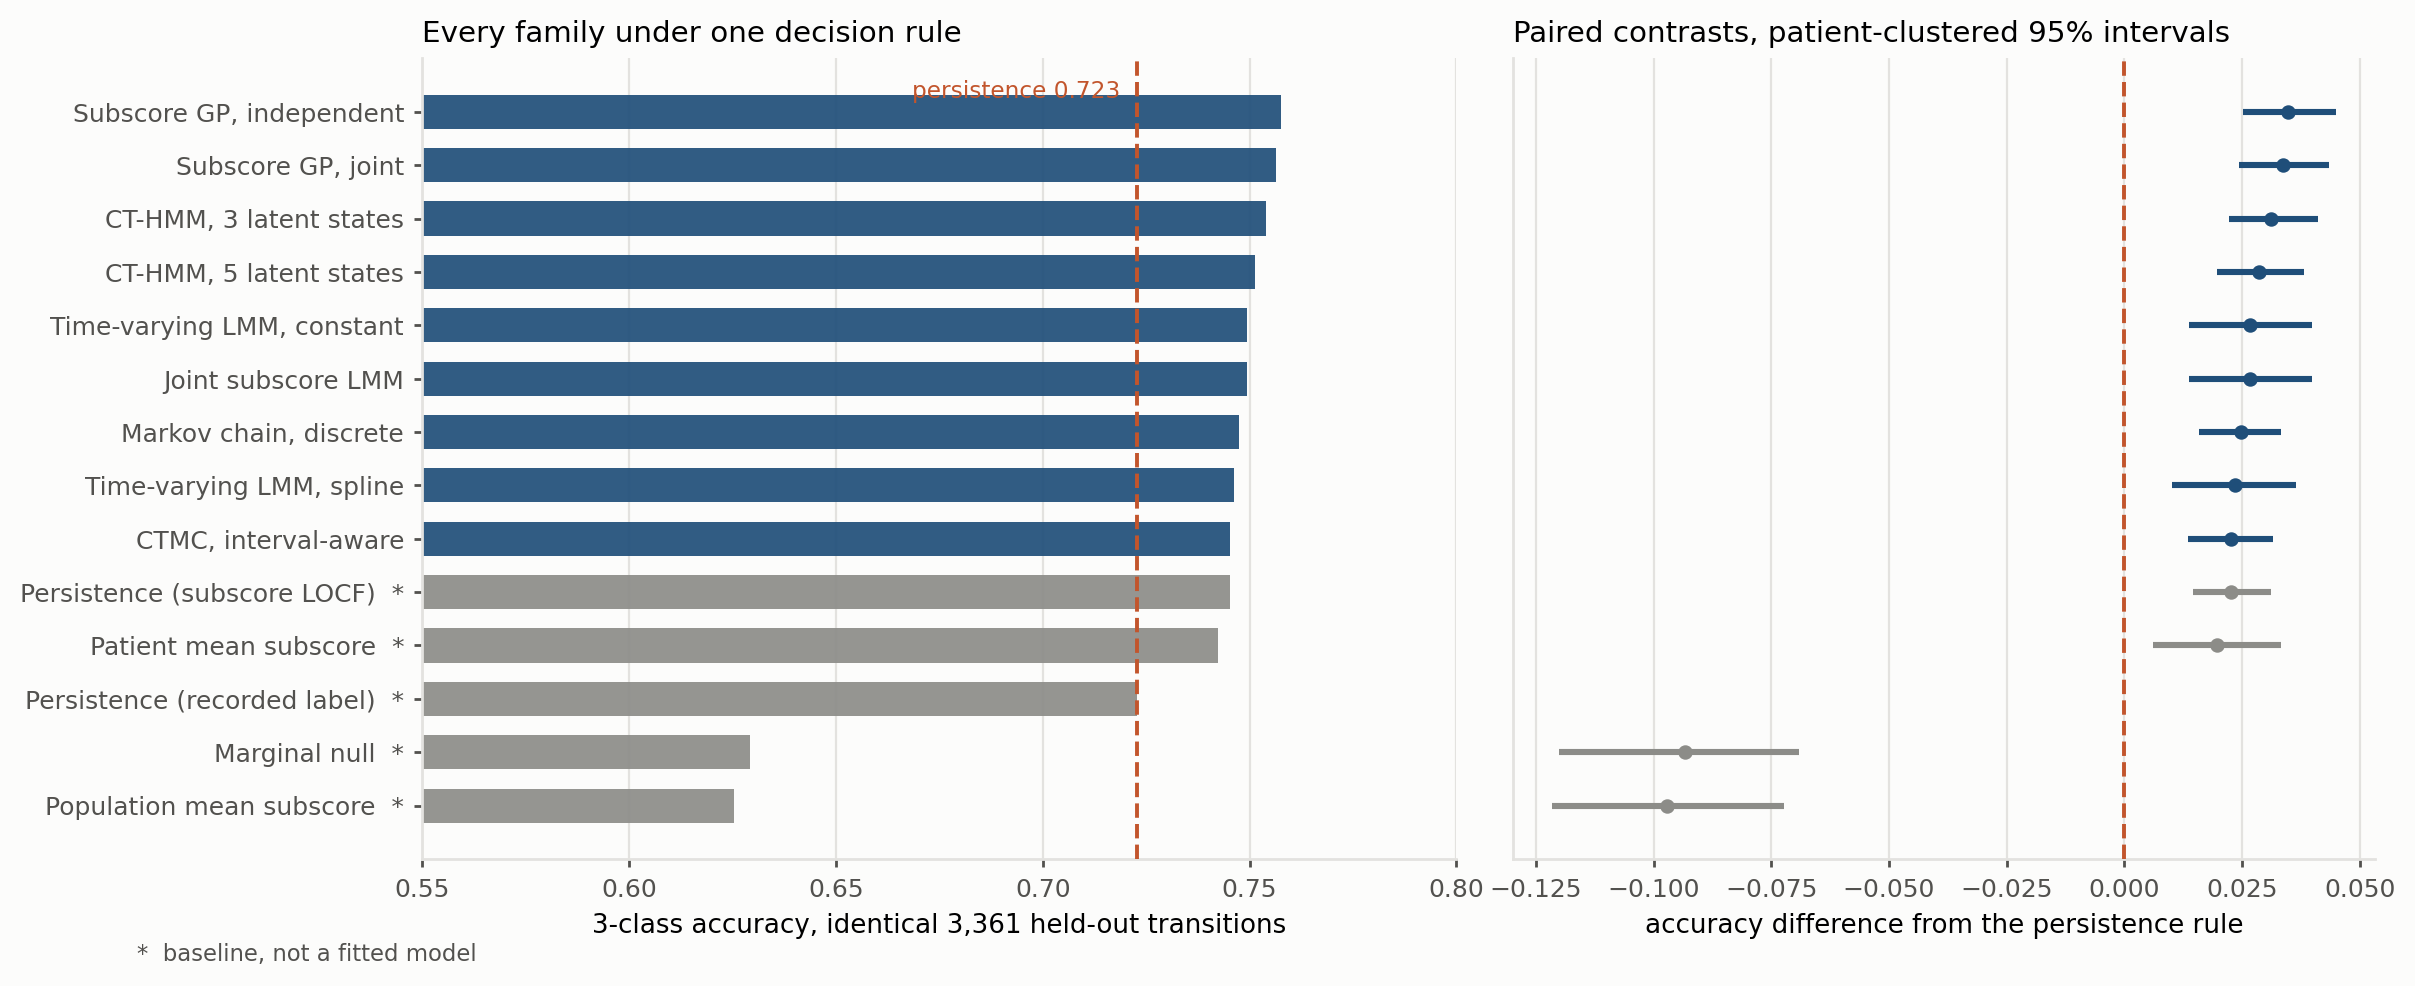
\includegraphics[width=\textwidth]{f11_harmonised.png}
\caption{Every specification under one decision rule on the identical 3,361
held-out transitions. \textbf{Left:} three-class accuracy; fitted models in dark,
baselines in grey, with the persistence rule marked. The $x$-axis is truncated at
0.55. \textbf{Right:} the paired accuracy difference of each specification from
the persistence rule, with patient-clustered bootstrap 95\% intervals. Panel
labels follow the source analysis: CT-HMM is the continuous-time hidden Markov
model of Section~\ref{sec:hmm} and CTMC the continuous-time Markov chain
of~\eqref{eq:ctmc}. Numerical values are in Table~\ref{tab:families}.}
\label{fig:families}
\end{figure}

\begin{table}[t]
\centering
\caption{Harmonised comparison of all specifications on the same 3,361 held-out
transitions from 934 patients, under one decision rule (argmax of the three-class
probability vector). ``Rec.\ Ind.'' is recall on the 332 Indeterminate outcomes.
$^{*}$The five-state hidden Markov model converged in only 404 of 934 folds and
is not a like-for-like estimate. $^{\dagger}$The persistence rule emits only zero
and one, so its log loss is clipped and it cannot be calibrated.}
\label{tab:families}
\scriptsize
\setlength{\tabcolsep}{4.5pt}
\begin{tabular}{@{}llrlrrrr@{}}
\toprule
Specification & Family & Acc. & $\Delta$ vs.\ persistence (95\% CI) & Brier & Log loss & Macro-F1 & Rec.\ Ind. \\
\midrule
\multicolumn{8}{@{}l}{\textit{Fitted models}}\\
Subscore GP, independent   & GP               & 0.7575 & $+0.0348$ \,(0.0252, 0.0450) & 0.3602 & 0.6537 & 0.5074 & 0.000 \\
Subscore GP, joint         & GP               & 0.7563 & $+0.0336$ \,(0.0243, 0.0436) & 0.3594 & 0.6518 & 0.5070 & 0.000 \\
HMM, 3 latent states       & latent HMM       & 0.7539 & $+0.0312$ \,(0.0223, 0.0411) & 0.3688 & 0.6726 & 0.5037 & 0.000 \\
HMM, 5 latent states$^{*}$ & latent HMM       & 0.7513 & $+0.0286$ \,(0.0196, 0.0381) & 0.3700 & 0.6746 & 0.5011 & 0.000 \\
Time-varying LMM, constant & mixed model      & 0.7495 & $+0.0268$ \,(0.0136, 0.0398) & 0.3826 & 0.6919 & 0.4977 & 0.000 \\
Joint subscore LMM         & mixed model      & 0.7495 & $+0.0268$ \,(0.0136, 0.0398) & 0.3826 & 0.6919 & 0.4977 & 0.000 \\
Markov chain, discrete     & observed-label   & 0.7474 & $+0.0247$ \,(0.0159, 0.0334) & 0.3896 & 0.7066 & 0.4929 & 0.000 \\
Time-varying LMM, spline   & mixed model      & 0.7462 & $+0.0235$ \,(0.0102, 0.0364) & 0.3794 & 0.6860 & 0.4937 & 0.000 \\
Markov chain, continuous   & observed-label   & 0.7453 & $+0.0226$ \,(0.0135, 0.0316) & 0.3925 & 0.7105 & 0.4909 & 0.000 \\
\addlinespace[3pt]
\multicolumn{8}{@{}l}{\textit{Baselines}}\\
Subscore LOCF              & baseline         & 0.7453 & $+0.0226$ \,(0.0146, 0.0311) & 0.3723 & 0.7556 & 0.4970 & 0.000 \\
Patient-mean subscore      & baseline         & 0.7423 & $+0.0196$ \,(0.0061, 0.0332) & 0.3802 & 0.7594 & 0.4903 & 0.003 \\
\textbf{Persistence}       & \textbf{baseline}& \textbf{0.7227} & ---                   & 0.5546 & 7.6620$^{\dagger}$ & \textbf{0.5559} & \textbf{0.193} \\
Marginal null              & baseline         & 0.6293 & $-0.0934$ \,($-0.1202$, $-0.0691$) & 0.5211 & 0.8756 & 0.2575 & 0.000 \\
Population-mean subscore   & baseline         & 0.6254 & $-0.0973$ \,($-0.1215$, $-0.0723$) & 0.5174 & 0.8716 & 0.3460 & 0.000 \\
\bottomrule
\end{tabular}

\end{table}

\paragraph{No fitted model recovers the Indeterminate class.}
Of the 332 Indeterminate outcomes, every fitted specification recovers none:
each predicts the class between zero and four times in 3,361 opportunities, and
per-class recall is 0.000 throughout. Only the persistence rule predicts it with
any frequency --- 334 times, recovering 19.3\% of them --- and in consequence
\textbf{the persistence rule attains the highest macro-F1 of any specification
tested} (0.5559 against 0.5074 for the best fitted model) while having the lowest
accuracy. Accuracy and macro-F1 rank the specifications in opposite orders,
because accuracy rewards abandoning a small middle class and macro-F1 does not.

\paragraph{The entire margin sits in one stratum.}
Stratifying each model's gain by the label recorded at the prediction point
localises the effect completely (Table~\ref{tab:margin},
Figure~\ref{fig:margin}). For the hidden Markov model, \textbf{94.3\% of its 105
net cases gained over persistence come from the 334 transitions (9.9\% of the
data) at which the current label was Indeterminate}, where persistence is right
19.2\% of the time and the model 48.8\%. Where the current label was TD it gained
six correct predictions out of 2,261; where the current label was PIGD it gained
\textbf{none at all} out of 766, the two rules achieving identical accuracy of
0.7023 on that stratum. The two approaches made the same call on 98.4\% of
current-TD and 96.9\% of current-PIGD transitions, against 0.3\% where the
current label was Indeterminate. The discrete Markov chain makes the point more
starkly: it predicted exactly what persistence predicted on 100\% of both outer
strata and took all 83 of its gained cases from the Indeterminate band.

\begin{table}[t]
\centering
\caption{Where each model's advantage over the persistence rule comes from,
decomposed by the label recorded at the prediction point. ``Cases gained'' is the
net number of additional correct predictions in that stratum.}
\label{tab:margin}
\footnotesize
\setlength{\tabcolsep}{3.5pt}
\begin{tabular}{@{}llrrrrrr@{}}
\toprule
Model & Stratum & $n$ & Share & Model acc. & Persist.\ acc. & Cases gained & Share of gain \\
\midrule
HMM, 3 latent states   & TD            & 2,261 & 67.3\% & 0.8107 & 0.8080 & 6   & 5.7\% \\
                       & Indeterminate & 334   & 9.9\%  & 0.4880 & 0.1916 & \textbf{99} & \textbf{94.3\%} \\
                       & PIGD          & 766   & 22.8\% & 0.7023 & 0.7023 & \textbf{0}  & 0.0\% \\
\addlinespace[2pt]
Subscore GP, indep.    & TD            & 2,261 & 67.3\% & 0.8120 & 0.8080 & 9   & 7.7\% \\
                       & Indeterminate & 334   & 9.9\%  & 0.4910 & 0.1916 & 100 & 85.5\% \\
                       & PIGD          & 766   & 22.8\% & 0.7128 & 0.7023 & 8   & 6.8\% \\
\addlinespace[2pt]
Markov chain, discrete & TD            & 2,261 & 67.3\% & 0.8080 & 0.8080 & 0   & 0.0\% \\
                       & Indeterminate & 334   & 9.9\%  & 0.4401 & 0.1916 & 83  & \textbf{100.0\%} \\
                       & PIGD          & 766   & 22.8\% & 0.7023 & 0.7023 & 0   & 0.0\% \\
\midrule
\multicolumn{8}{@{}l}{\textit{Share of predictions identical to the persistence rule}}\\
HMM, 3 latent states   & \multicolumn{3}{l}{TD 98.4\%} & \multicolumn{2}{l}{Indeterminate 0.3\%} & \multicolumn{2}{l}{PIGD 96.9\%} \\
Subscore GP, indep.    & \multicolumn{3}{l}{TD 97.2\%} & \multicolumn{2}{l}{Indeterminate 0.0\%} & \multicolumn{2}{l}{PIGD 97.4\%} \\
Markov chain, discrete & \multicolumn{3}{l}{TD 100.0\%} & \multicolumn{2}{l}{Indeterminate 0.0\%} & \multicolumn{2}{l}{PIGD 100.0\%} \\
\bottomrule
\end{tabular}

\end{table}

\begin{figure}[t]
\centering
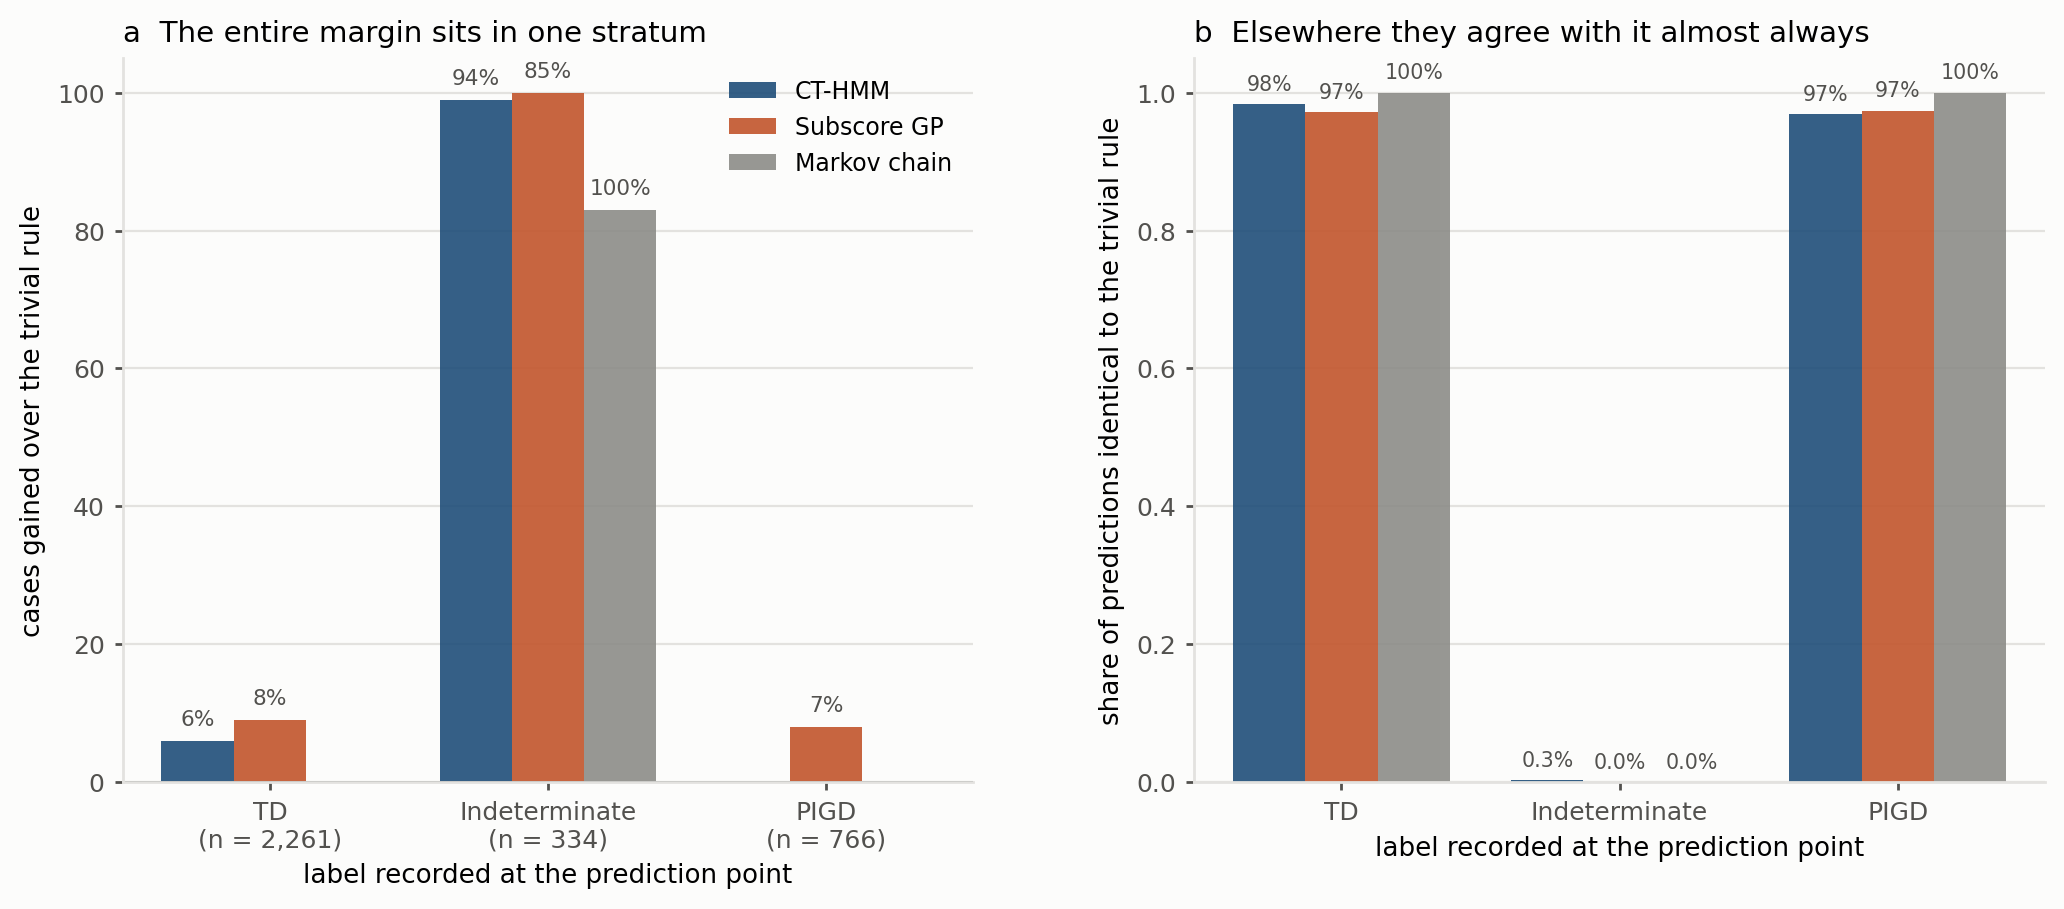
\includegraphics[width=\textwidth]{f12_margin.png}
\caption{Where each model's advantage over the persistence rule comes from.
(\textbf{a}) Extra correct predictions over persistence in each stratum; the
percentage above each bar is that stratum's share of the model's total gain.
(\textbf{b}) Share of predictions identical to persistence in each stratum.
Outside the Indeterminate band the fitted models reproduce the trivial rule
almost exactly. Panel labels follow the source analysis: CT-HMM is the three-state
hidden Markov model, Subscore GP the independent subscore Gaussian process, and
Markov chain the discrete-time chain.}
\label{fig:margin}
\end{figure}

\paragraph{What the models are actually doing.} They are not predicting
progression better than the trivial rule. On 90\% of transitions they reproduce
it. On the remaining tenth they decline to repeat a class that is rarely
repeated, and that accounts for essentially all of their advantage. The accuracy
ceiling is therefore not a property of any model; it is set by how often the next
label contradicts the history, which is a property of the label.

\subsection{Does a richer observation help?}
\label{sec:richer}

The harmonised comparison varies the model while holding the observation
essentially fixed --- a label, or the two subscores it is computed from. This
section varies the observation.

\subsubsection{The two-class task, and what a latent state is worth}

Removing the Indeterminate outcomes leaves 3,029 transitions from 899 patients on
which the target is TD or PIGD (Table~\ref{tab:twoclass}). The hidden Markov
model reaches 0.8369 (0.8204--0.8541), a direct logistic model with the history
and the interval 0.8359, persistence of the last non-Indeterminate label 0.8336,
the discrete chain 0.8293 and a two-class prior 0.6983.

The pre-specified contrasts separate what each ingredient is worth. Holding the
observed process interval-aware, adding a \emph{latent state} is worth $+0.0092$
($+0.0003$ to $+0.0179$) --- the one structural comparison in this paper whose
interval excludes zero. Holding the chain in the observed label, adding
\emph{elapsed time} is worth $-0.0017$ ($-0.0039$ to $+0.0003$), that is nothing;
in the discriminative family the same ingredient is worth $+0.0165$ ($+0.0112$ to
$+0.0217$). A latent generative model and a direct discriminative one are
indistinguishable ($+0.0010$, $-0.0054$ to $+0.0075$), and the hidden Markov
model's advantage over persistence on this task is $+0.0033$ ($-0.0037$ to
$+0.0100$), with an interval containing zero.

The rise from 0.754 to 0.837 between the three-class and the two-class task is
largely the removal of an outcome the models never predict, not better
prediction.

\begin{table}[t]
\centering
\caption{Next-visit TD-against-PIGD prediction on the 3,029 eligible transitions
of 899 patients, leave-one-patient-out. $^{\dagger}$The persistence rule's log
loss is undefined and is reported clipped.}
\label{tab:twoclass}
\small
\begin{tabular}{@{}lrlrr@{}}
\toprule
Model & Accuracy & 95\% CI & Brier & Log loss \\
\midrule
Hidden Markov model (latent, interval-aware) & 0.8369 & (0.8204, 0.8541) & 0.1214 & 0.3961 \\
Direct logistic (history $+$ interval)       & 0.8359 & (0.8195, 0.8529) & 0.1225 & 0.4003 \\
Persistence (last non-Indeterminate label)   & 0.8336 & (0.8173, 0.8510) & 0.1598 & $4.193^{\dagger}$ \\
Markov chain, discrete-time                  & 0.8293 & (0.8129, 0.8468) & 0.1328 & 0.4314 \\
Markov chain, continuous-time                & 0.8277 & (0.8114, 0.8451) & 0.1343 & 0.4346 \\
Direct logistic (history only)               & 0.8194 & (0.8019, 0.8372) & 0.1244 & 0.4055 \\
Marginal (two-class prior)                   & 0.6983 & (0.6703, 0.7278) & 0.2111 & 0.6134 \\
\midrule
\multicolumn{5}{@{}l}{\textit{Pre-specified paired contrasts (model a $-$ model b) on identical cases}}\\
\multicolumn{2}{@{}l}{Latent state, observed process held interval-aware} & \multicolumn{3}{l}{$+0.0092$ \,($+0.0003$, $+0.0179$) \quad \textbf{excludes zero}} \\
\multicolumn{2}{@{}l}{Elapsed time, observed-label chain} & \multicolumn{3}{l}{$-0.0017$ \,($-0.0039$, $+0.0003$)} \\
\multicolumn{2}{@{}l}{Elapsed time, discriminative family} & \multicolumn{3}{l}{$+0.0165$ \,($+0.0112$, $+0.0217$) \quad \textbf{excludes zero}} \\
\multicolumn{2}{@{}l}{Latent generative $-$ discriminative} & \multicolumn{3}{l}{$+0.0010$ \,($-0.0054$, $+0.0075$)} \\
\multicolumn{2}{@{}l}{Hidden Markov model $-$ persistence} & \multicolumn{3}{l}{$+0.0033$ \,($-0.0037$, $+0.0100$)} \\
\multicolumn{2}{@{}l}{Hidden Markov model $-$ marginal prior} & \multicolumn{3}{l}{$+0.1387$ \,($+0.1107$, $+0.1665$) \quad \textbf{excludes zero}} \\
\bottomrule
\end{tabular}

\end{table}

\subsubsection{A discrete latent clinical state destroys information}

Replacing the label alphabet with a Gaussian emission over ten standardised
clinical measurements makes the prediction \emph{worse}, by a wide margin. On
2,091 identical two-class cases, a six-state model reaches 0.7255
(0.6960--0.7534) and an eight-state model 0.7336 (0.7062--0.7607), against 0.8384
(0.8183--0.8568) for the subtype-history model on the same cases: paired
differences of $-0.1130$ ($-0.1438$ to $-0.0807$) and $-0.1048$ ($-0.1357$ to
$-0.0757$). The loss is concentrated where the current label is PIGD (accuracy
0.397 against 0.787).

The cause is the bottleneck, not the measurements. A direct logistic model on the
\emph{same} ten measurements and the interval reaches 0.8307 (0.8086--0.8515)
with the best Brier score and log loss of any model on that evaluation set:
$+0.1052$ ($+0.0756$ to $+0.1338$) over the latent model, and $-0.0077$
($-0.0204$ to $+0.0046$) against the subtype-history model. Restricting it to the
tremor and PIGD scores alone changes nothing ($-0.0010$, $-0.0114$ to $+0.0091$).
Eight of the ten measurements therefore add nothing, and forcing ten continuous
measurements through a handful of discrete states discards the within-patient
variation the prediction needs (Supplementary~\ref{sup:clinical}).

\subsubsection{A continuous profile ties on accuracy and wins on ranking}

A continuous nine-domain level-and-rate profile is a better model of the clinical
record than assuming no change: $+0.0733$ log-density per domain observation over
last-observation-carried-forward ($+0.0657$ to $+0.0813$), better in 75.1\% of
predictions (Table~\ref{tab:profile}a). Modelling the rate of change contributes
$+0.0040$ ($+0.0019$ to $+0.0062$) and medication as an input $+0.0058$
($+0.0041$ to $+0.0075$) --- together under a sixth of the gain, with most of it
coming from the level being filtered across a patient's history rather than read
off the most recent visit. The fitted medication coefficient is positive in eight
of nine domains, which is confounding by indication: patients who start levodopa
are those who are worsening, and no coefficient on it supports a causal reading.

On the next label, the profile is \emph{indistinguishable} from the latent-state
model: 0.8404 (0.8248--0.8566) against 0.8371 (0.8202--0.8540), a paired
difference of $+0.0033$ ($-0.0050$ to $+0.0112$) on 3,020 matched transitions
(Table~\ref{tab:profile}b). Its simplest variant --- a random walk on the levels,
with no rate and no medication --- reaches 0.8440, as good as its richest.

On \emph{ranking} it is clearly better: AUC 0.8902 (0.8748--0.9053) against
0.8583 (0.8411--0.8755), a paired difference of $+0.0319$ ($+0.0229$ to
$+0.0419$), and better in every current-label stratum
(Figure~\ref{fig:roc}). We note that this one comparison spans two validation
designs, which favours the hidden Markov model.

\begin{table}[t]
\centering
\caption{The continuous nine-domain profile. Panel (d) coordinates were selected
on the same data against which they were compared, so each difference is an upper
bound. $^{\ddagger}$The investigator cognitive diagnosis is not fully independent
of the inputs and is reported for completeness.}
\label{tab:profile}
\small
\begin{tabular}{@{}llrl@{}}
\toprule
 & Comparison & Estimate & 95\% CI \\
\midrule
\multicolumn{4}{@{}l}{\textit{(a) Predicting the next visit's clinical record (log-density per domain observation)}}\\
 & Profile $-$ last observation carried forward & $+0.0733$ & ($+0.0657$, $+0.0813$) \\
 & Profile $-$ population mean trajectory       & $+0.3889$ & ($+0.3628$, $+0.4167$) \\
 & Rate-of-change component                     & $+0.0040$ & ($+0.0019$, $+0.0062$) \\
 & Medication as an input                       & $+0.0058$ & ($+0.0041$, $+0.0075$) \\
\addlinespace[3pt]
\multicolumn{4}{@{}l}{\textit{(b) Two-class next-label accuracy on 3,020 matched transitions (898 patients)}}\\
 & Profile: level only (random walk)            & 0.8440 & (0.8285, 0.8598) \\
 & Profile: level $+$ rate $+$ medication       & 0.8404 & (0.8248, 0.8566) \\
 & Hidden Markov model                          & 0.8371 & (0.8202, 0.8540) \\
 & Persistence                                  & 0.8338 & (0.8167, 0.8509) \\
 & Profile $-$ hidden Markov model              & $+0.0033$ & ($-0.0050$, $+0.0112$) \\
\addlinespace[3pt]
\multicolumn{4}{@{}l}{\textit{(c) Threshold-free discrimination of next-visit PIGD (AUC-ROC)}}\\
 & Profile                                      & 0.8902 & (0.8748, 0.9053) \\
 & Hidden Markov model                          & 0.8583 & (0.8411, 0.8755) \\
 & Profile $-$ hidden Markov model              & $+0.0319$ & ($+0.0229$, $+0.0419$) \\
\addlinespace[3pt]
\multicolumn{4}{@{}l}{\textit{(d) Discrimination of later-recorded outcomes: best single level coordinate vs the label}}\\
 & Hoehn \& Yahr $\geq 3$ ($n{=}761$, 127 events) & $+0.1052$ & ($+0.0540$, $+0.1557$) \\
 & Mild cognitive impairment ($n{=}818$, 298)     & $+0.1605$ & ($+0.1093$, $+0.2132$) \\
 & Investigator cognitive diagnosis$^{\ddagger}$ ($n{=}816$, 327) & $+0.1194$ & ($+0.0690$, $+0.1687$) \\
 & Motor complications ($n{=}736$, 470)           & $+0.0272$ & ($-0.0394$, $+0.0941$) \\
 & Best \emph{rate} coordinate, any outcome       & \multicolumn{2}{l}{$+0.033$ to $+0.053$, every interval contains zero} \\
\bottomrule
\end{tabular}

\end{table}

\begin{figure}[t]
\centering
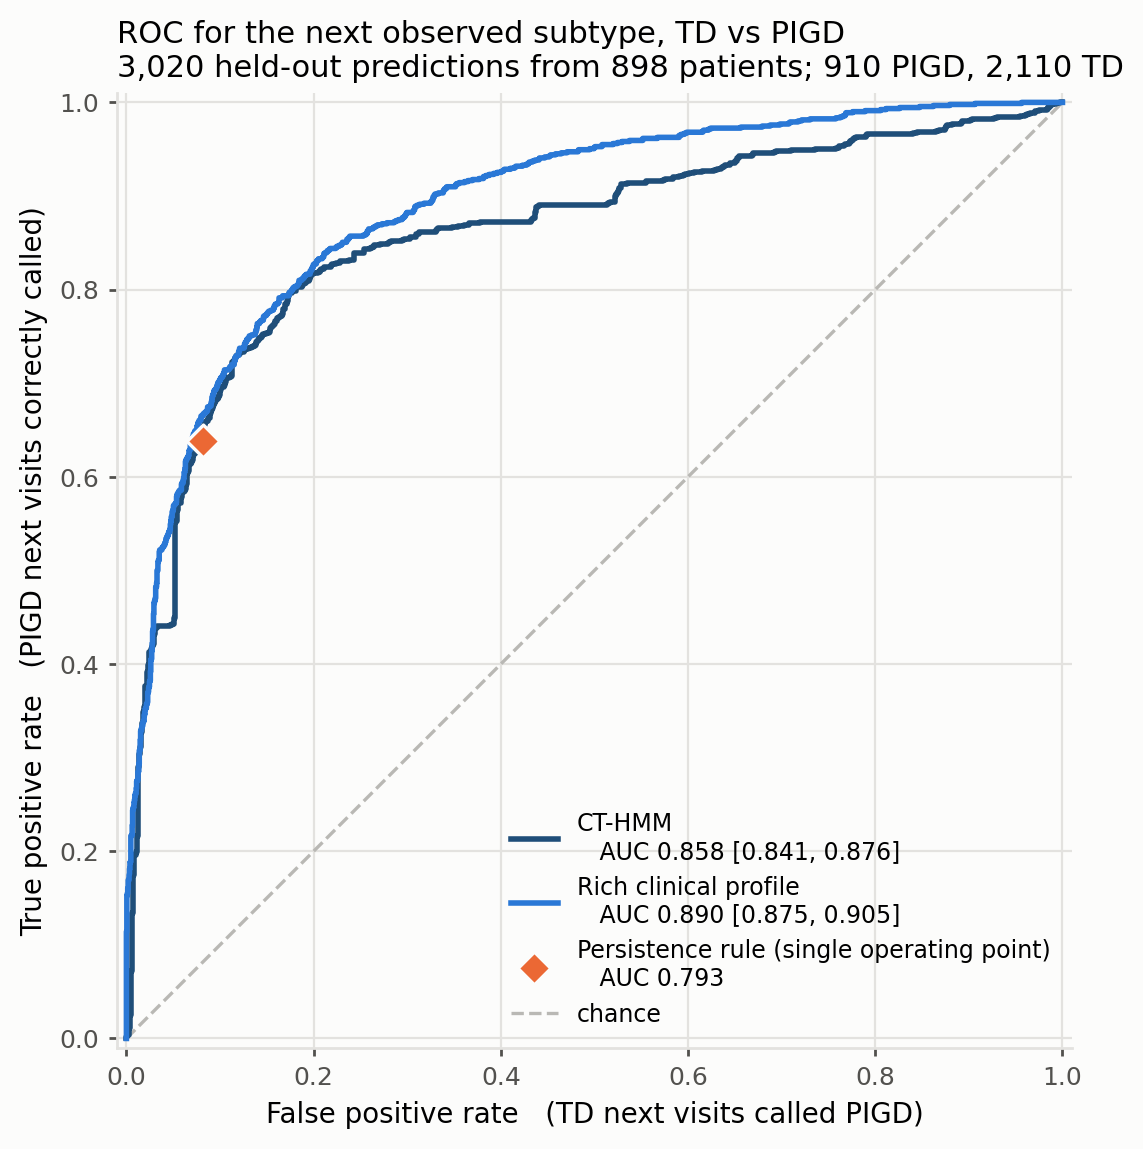
\includegraphics[width=0.74\textwidth]{f13_roc.png}
\caption{ROC curves for next-visit PIGD against TD on 3,020 matched transitions:
the nine-domain clinical profile, the hidden Markov model on the subtype history,
and the persistence rule. The profile ranks a PIGD visit above a TD visit
substantially better than the latent-state model while calling them no more
accurately at the 0.5 threshold.}
\label{fig:roc}
\end{figure}

\paragraph{The representation carries information the label does not.}
Against outcomes recorded later and never used in fitting, single coordinates of
the profile discriminate better than the subtype label
(Table~\ref{tab:profile}d, Figure~\ref{fig:outcomes}): Hoehn \& Yahr stage 3 or
worse at AUC 0.685 against the label's 0.579 ($+0.105$, $+0.054$ to $+0.156$),
and mild cognitive impairment at 0.710 against 0.549 ($+0.161$, $+0.109$ to
$+0.213$). For motor complications, which the label discriminates at chance
(0.504), the difference is $+0.027$ ($-0.039$ to $+0.094$). \textbf{No rate
coordinate beats the label by an interval that excludes zero} on any outcome. The
representation is genuinely multidimensional: seven of nine principal components
are required for 90\% of the across-patient variance of either the levels or the
rates.

\begin{figure}[t]
\centering
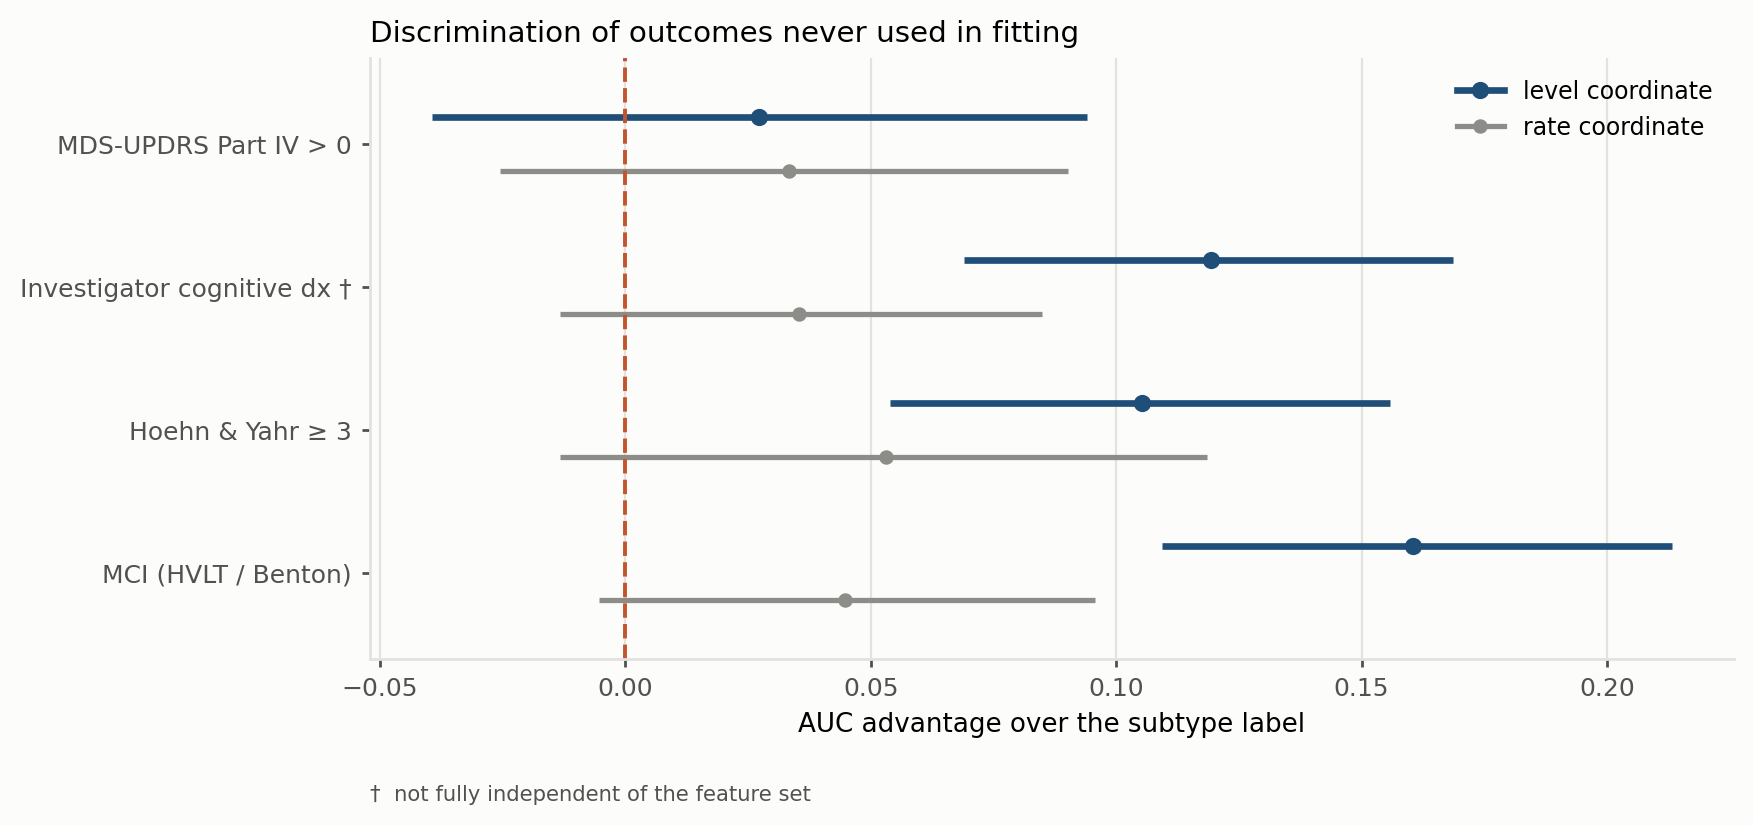
\includegraphics[width=0.86\textwidth]{f15_outcomes.png}
\caption{Discrimination of subsequently recorded clinical outcomes by the best
single profile coordinate against the subtype label. Coordinates were selected on
the same data against which they were compared, so each difference is an upper
bound. The level coordinates carry prognostic information about staging and
cognition that the categorical label does not; the rate coordinates do not.}
\label{fig:outcomes}
\end{figure}

\subsubsection{The same dissociation inside one model family}

The profile comparison changes the model class, the observation and the
validation design at once. To isolate the observation we widened only what the
latent-state model sees, leaving its latent process and decision rule untouched:
the observation becomes the pair (subtype, ratio band).

The result reproduces the dissociation exactly (Table~\ref{tab:bands},
Figure~\ref{fig:banded}). Accuracy does not improve --- $-0.0053$ ($-0.0134$ to
$+0.0034$) at band width 0.10, and between 0.832 and 0.836 at every width against
0.837 unbanded, every contrast containing zero. Calibration gets \emph{worse}:
the calibration gap rises from 0.0065 to 0.022--0.029. But AUC rises at every
width, by $+0.015$ to $+0.020$, every interval excluding zero. The gain is
concentrated in the current-TD stratum (0.669 to 0.750) and among cases with one
prior visit; it is absent from the Indeterminate and PIGD strata, and the
band-width sweep finds an interior optimum near 0.30 that is worth a few
thousandths of AUC and nothing on the two ranking metrics that weight the
operating region (Supplementary~\ref{sup:bands}).

An emission diagnostic explains why. Within each subtype, the band distributions
of the three latent states differ by total-variation distances of up to 0.66, so
the band genuinely carries information about the latent state --- but what it
carries re-orders cases that are already on the TD side of the boundary rather
than moving cases across it.

\begin{table}[t]
\centering
\caption{Adding the ratio band to the observation alphabet of the hidden Markov
model, at five band widths, on the same 3,029 two-class transitions. The latent
process and the decision rule are unchanged; only the observation differs. pAUC
is the partial area under the curve for false-positive rate at most 0.2.}
\label{tab:bands}
\small
\setlength{\tabcolsep}{5pt}
\begin{tabular}{@{}lrrrrrrr@{}}
\toprule
Observation alphabet & Cat. & Par. & Accuracy & AUC-ROC & PR-AUC & pAUC & Calib.\ gap \\
\midrule
Subtype only                 & 3  & 14  & \textbf{0.8369} & 0.8587 & 0.7496 & 0.7883 & \textbf{0.0065} \\
Subtype $\times$ band, 0.05  & 73 & 224 & 0.8336 & 0.8739 & 0.7330 & 0.7802 & 0.0250 \\
Subtype $\times$ band, 0.10  & 44 & 137 & 0.8316 & 0.8758 & 0.7398 & 0.7823 & 0.0285 \\
Subtype $\times$ band, 0.20  & 29 & 92  & 0.8336 & 0.8775 & \textbf{0.7540} & 0.7868 & 0.0240 \\
Subtype $\times$ band, 0.30  & 24 & 77  & 0.8359 & \textbf{0.8784} & 0.7523 & \textbf{0.7892} & 0.0224 \\
Subtype $\times$ band, 0.50  & 20 & 65  & 0.8320 & 0.8765 & 0.7409 & 0.7827 & 0.0291 \\
\midrule
\multicolumn{8}{@{}l}{\textit{Paired contrasts against the subtype-only model}}\\
\multicolumn{3}{@{}l}{Accuracy, band 0.10} & \multicolumn{5}{l}{$-0.0053$ \,($-0.0134$, $+0.0034$) \quad interval contains zero} \\
\multicolumn{3}{@{}l}{AUC-ROC, every width} & \multicolumn{5}{l}{$+0.0151$ to $+0.0197$ \quad every interval excludes zero} \\
\multicolumn{3}{@{}l}{PR-AUC, band 0.30} & \multicolumn{5}{l}{$+0.0027$ \,($-0.0170$, $+0.0214$) \quad interval contains zero} \\
\multicolumn{3}{@{}l}{Partial AUC, band 0.30} & \multicolumn{5}{l}{$+0.0009$ \,($-0.0074$, $+0.0090$) \quad interval contains zero} \\
\addlinespace[2pt]
\multicolumn{8}{@{}l}{\textit{Where the AUC gain sits (band 0.10 vs subtype only)}}\\
\multicolumn{3}{@{}l}{Current label TD ($n{=}2{,}080$)} & \multicolumn{5}{l}{0.669 $\to$ 0.750} \\
\multicolumn{3}{@{}l}{Current label Indeterminate ($n{=}270$)} & \multicolumn{5}{l}{0.633 $\to$ 0.635} \\
\multicolumn{3}{@{}l}{Current label PIGD ($n{=}679$)} & \multicolumn{5}{l}{0.665 $\to$ 0.673} \\
\bottomrule
\end{tabular}

\end{table}

\begin{figure}[t]
\centering
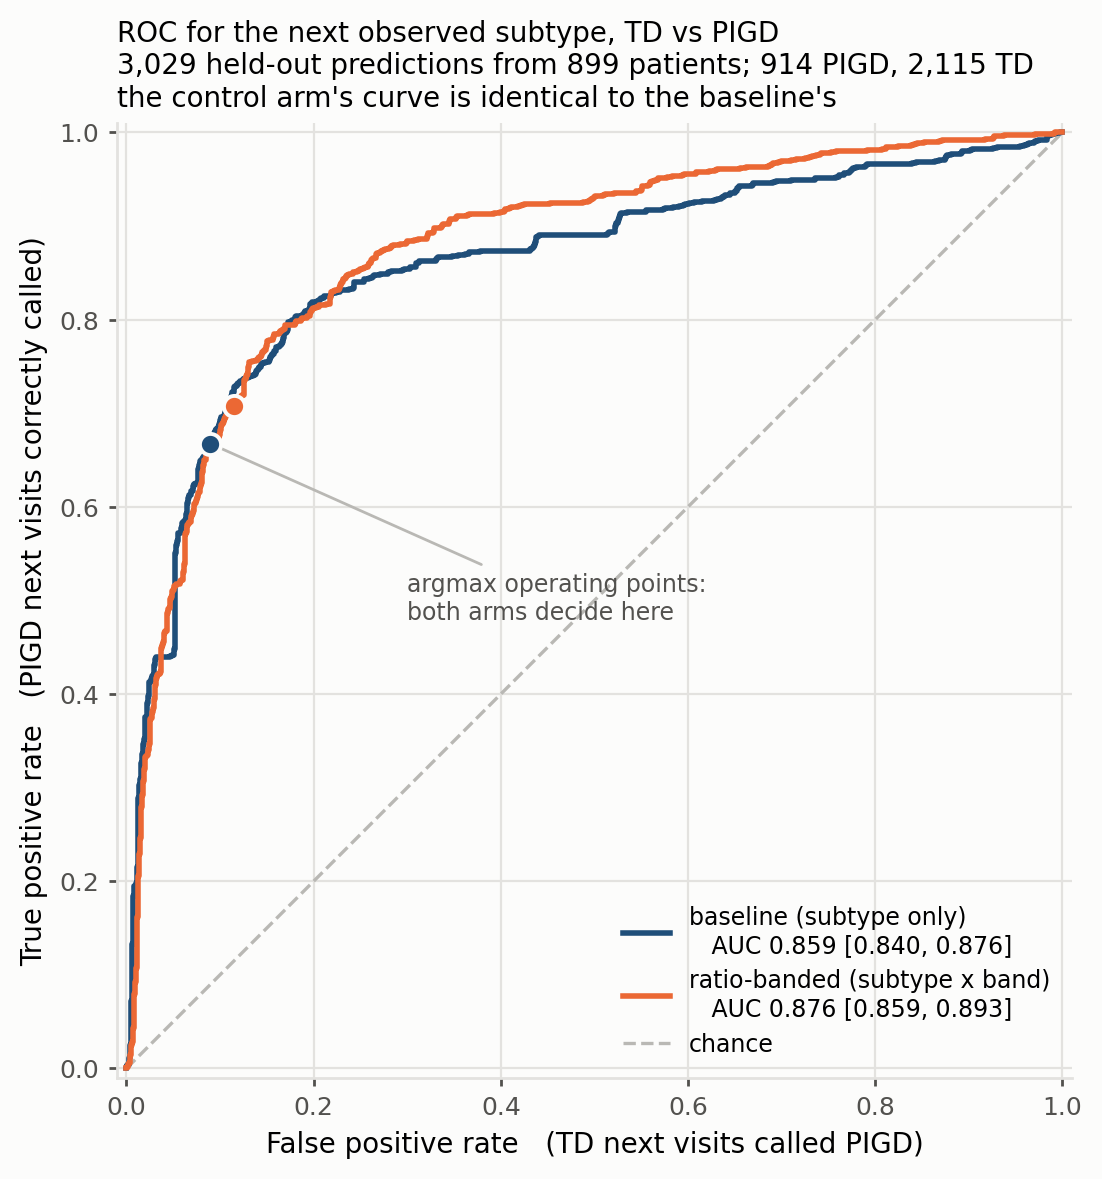
\includegraphics[width=0.74\textwidth]{f14_banded_roc.png}
\caption{ROC curves of the ratio-banded and the subtype-only hidden Markov model
on the same 3,029 transitions. Widening the observation alphabet to carry the
ratio band raises the area under the curve by $+0.017$ ($+0.009$ to $+0.026$)
while leaving accuracy unchanged and calibration worse --- the same dissociation
the nine-domain profile shows, obtained here inside one model family with one
latent process.}
\label{fig:banded}
\end{figure}

\paragraph{Interpretation.} Richer observations of the patient do improve the
\emph{ordering} of cases on either side of the decision boundary. They do not
improve the \emph{call} at the boundary, and they can make the probabilities
worse. Because the second demonstration holds the model class, the latent process
and the decision rule fixed, the pattern cannot be attributed to a change of
model family.

\subsection{What the ceiling is not}
\label{sec:ceiling}

Four candidate explanations for the accuracy ceiling remain. Each was tested and
each fails.

\paragraph{It is not a shortage of history.} Truncating the latent-state model's
prediction-time history to the last two visits leaves performance
indistinguishable from the full record on every metric: accuracy $-0.0041$
($-0.0189$ to $+0.0100$), balanced accuracy $-0.0063$, AUC $-0.0045$, Brier
$+0.0051$ and log loss $+0.0112$, all five intervals containing zero. A single
visit \emph{is} measurably worse --- accuracy $-0.0218$ ($-0.0423$ to $-0.0014$)
and AUC $-0.0617$ ($-0.0858$ to $-0.0385$) --- so the second visit carries real
information while the fourth and beyond do not. The nine-domain profile behaves
identically ($-0.0007$, $-0.0102$ to $+0.0085$), and substituting the current
visit's medication for the next visit's changes accuracy by $-0.0013$, which also
disposes of a concern about that input (Supplementary~\ref{sup:history}).

\paragraph{It is not the training regime.} Refitting the latent-state model on
two-visit sliding windows, so that training matches the restricted input, does
not help and degrades the probabilities: balanced accuracy $-0.0312$ ($-0.0441$
to $-0.0183$), AUC $-0.0210$, log loss $+0.0397$ against the full-sequence model.
A $2\times2$ design attributes the loss to the change in \emph{training}
($-0.0248$ balanced accuracy with prediction history held fixed) rather than to
the history restriction ($-0.0064$, interval containing zero). The fitted
parameters show why: trained on windows, the initial Indeterminate probability
falls from 0.155 to 0.044 and the Indeterminate emission diagonal rises off its
floor, because a window's first visit is treated as a draw from the initial
distribution and the model learns to explain every window's start rather than the
cohort's baseline.

\paragraph{It is not a property of early disease.} Across nine prediction stages
with at least 66 targets each, \textbf{no change in accuracy from stage 1
excludes zero} for either the latent-state model or the profile, and of 24
pre-specified paired tests exactly one interval excludes zero (the profile's
balanced accuracy at stage 1, $+0.046$). Balanced accuracy does rise with stage
for every model including persistence, but so does the PIGD share of outcomes,
from 23\% at stage 1 to 48\% at stage 9: the trend is cohort composition, not
learning. Within patients, the late-minus-early change in accuracy is $-0.024$
($-0.075$ to $+0.028$; Supplementary~\ref{sup:stage}).

\paragraph{It is not hidden by aggregation.} Weighting each patient equally rather
than each visit changes the headline little --- mean per-patient accuracy 0.834
(0.817--0.852) against a visit-level 0.839 --- but the distribution is strongly
bimodal rather than concentrated near that mean (Figure~\ref{fig:patient}). Of
898 patients, 572 (63.7\%) are predicted correctly at every eligible visit and 45
(5.0\%) at none; the median per-patient accuracy is 1.000.

The dominant source of variation is whether a patient's recorded label changes at
all. Patients whose eligible outcomes were all TD averaged 0.944, and those with
an even mixture of TD and PIGD outcomes averaged 0.468. \textbf{The persistence
rule shows almost the same gradient on the same groups --- 0.970 and 0.480 --- so
this describes the label sequence rather than model behaviour.} At the patient
level the paired comparisons repeat the visit-level ones, with 660 to 828 of the
matched patients unchanged under every contrast. These groupings were defined
after the predictions were generated and from recorded labels only; the analysis
is descriptive and is reported as exploratory.

\begin{figure}[t]
\centering
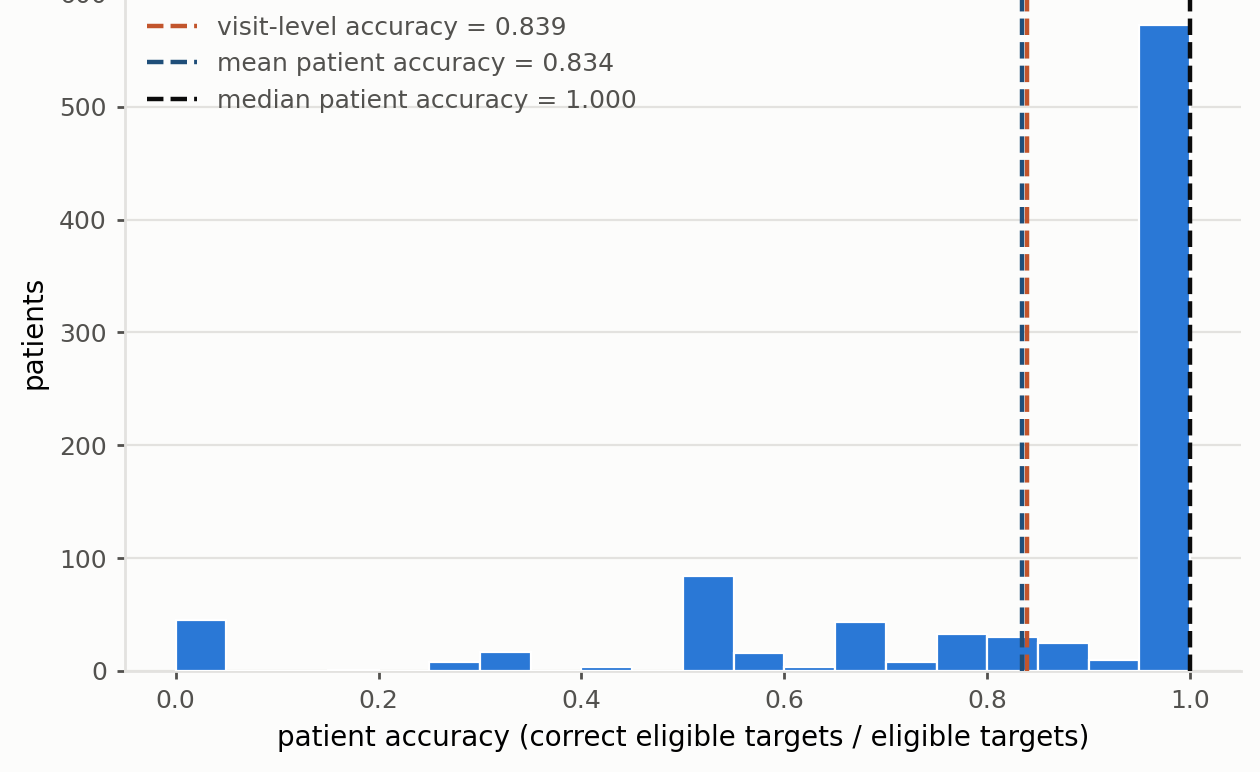
\includegraphics[width=0.80\textwidth]{f16_patient.png}
\caption{Distribution of per-patient two-class accuracy for the nine-domain
profile with the full history (898 patients, 3,021 eligible targets). The
distribution is bimodal rather than concentrated near its mean: 63.7\% of
patients are predicted correctly at every eligible visit and 5.0\% at none. The
persistence rule produces almost the same distribution.}
\label{fig:patient}
\end{figure}

% ====================================================================
\section{Discussion}
% ====================================================================

\subsection{Principal interpretation}
On one cohort and one evaluation protocol, model families embodying substantially
different assumptions predicted the next recorded motor subtype within 1.22
accuracy points of one another, with the best gaining about three points over a
rule that repeats the current label. Essentially all of that shared advantage
arose on the one tenth of assessments recorded Indeterminate, and none of the
fitted models recovered that class. Over the same transitions, more than a third
of observed subtype changes were reversed at the following visit, a quarter of
same-visit labels moved with the examination state alone, and moving the decision
thresholds by less than the spacing of attainable ratio values relabelled a fifth
of patients.

Read together, these results locate the limit on longitudinal subtype prediction
in this cohort in the reliability and representation of the label rather than in
the capacity of the models. That is a claim about this target, in this cohort,
under this protocol. It is not a claim that model capacity is irrelevant in
general, and it is not a claim that the families compared here exhaust what could
be tried.

\subsection{Observed label transitions are not biological progression}
The distinction this paper insists on is between a change in the recorded label
and a change in the patient. Three results bear on it directly, and none of them
requires a model.

A third of observed changes are undone at the very next assessment, and reversion
is concentrated in changes that touch the Indeterminate band, where it reaches
0.50 to 0.56. The estimated incidence of conversion to PIGD halves when the
conversion is required to hold across two consecutive visits. And the same visit,
scored from the OFF and the ON examination, carries a different label a quarter of
the time. A change of recorded subtype is therefore a composite of phenotypic
movement, rating variability and the state in which the examination happened to
be performed, and this design cannot separate them.

The practical consequence is that a conversion endpoint defined on a single
assessment overstated incidence in this cohort by roughly a factor of two
relative to one requiring a sustained change. That belongs in a study protocol
rather than in the analysis.

\subsection{Why the observed-label chain is the wrong model, and why fixing it
barely helps}
The recorded label fails a first-order Markov test in all three states, so a chain
in the label is rejected by the data. The natural repair --- a latent state read
through a misclassification matrix --- is supported on information criteria by a
wide margin, beats the chain in 10 of 10 resamples on held-out log-likelihood,
and is worth $+0.009$ accuracy on the two-class task with an interval that
excludes zero.

And yet it is worth only three accuracy points over a parameter-free rule on the
three-class task, of which 94\% comes from one stratum covering a tenth of the
data. The repair is correct and the gain is small, which is itself informative:
the thing the latent layer fixes --- the label's failure to be a sufficient
statistic for its own past --- is not the thing that limits accuracy.

\subsection{Bayesian trend modelling describes the population, not the patient}
The growth model's population slope of $-0.093$ per year is estimated precisely,
with a credible interval of $-0.116$ to $-0.068$ and a posterior probability of
being negative of 1.000. It is also nearly uninformative about any individual:
the between-patient SD of slopes is 0.103 per year, comparable to the population
slope itself, so the fitted distribution of individual rates spans both signs.

This is the general hazard in reading a population trend as a prediction, and it
is sharpened here by the second finding: the model's total residual SD is 1.14
against an Indeterminate band 0.25 wide. Even a perfectly estimated individual
trajectory would place the next observation almost anywhere relative to that
band. The model cannot separate observation noise from process noise --- the two
additive terms are not identified --- which is precisely the decomposition a
label-prediction model would need.

\subsection{Why Gaussian process performance differs across the ratio and the
subscores}
The flexible kernel beats the linear trend on the ratio by a clear margin and
loses to a trivial rule on the PIGD subscore. Three properties of the targets
explain the reversal.

The ratio is volatile (median within-patient SD 0.76) and benefits from a model
that can follow excursions; the subscores are far better behaved (0.19 and 0.14),
leaving less for flexibility to capture. The PIGD subscore has an atom at zero
covering a sixth of visits, which persistence respects exactly and a continuous
Gaussian cannot represent at all --- at those visits persistence predicts below
0.1 at 62\% of them and the Gaussian process never does. And the ratio is
undefined precisely at those visits, so the ratio model never sees the cases on
which the subscore model loses.

The reversal is therefore a statement about the match between a likelihood and a
target, not about the merit of flexible trajectory modelling. It is also the
clearest argument in this paper for the direction described in
Section~\ref{sec:future}.

\subsection{Richer observations improve ranking, not accuracy}
Two independent demonstrations give the same answer. A continuous nine-domain
profile ties with the latent-state model on the next label while raising AUC by
$+0.032$; a ratio band added inside the latent-state model's own observation
alphabet leaves accuracy unchanged, worsens calibration, and raises AUC by
$+0.017$ at every band width. The second holds the model class, the latent
process and the decision rule fixed, so the dissociation is a property of the
observation rather than of the architecture.

The mechanism is visible in the emission diagnostic: the extra information
re-orders cases that are already on one side of the decision boundary rather than
moving cases across it. A target defined by thresholding is insensitive to
information that does not bear on which side of the threshold a case falls.

\subsection{What the profile carries that the label does not}
The constructive finding of the programme is a dissociation of a different kind.
The nine-domain representation ties with the latent-state model on predicting the
label, yet its level coordinates discriminate later-recorded Hoehn \& Yahr stage
3 or worse and mild cognitive impairment substantially better than the label does
($+0.105$ and $+0.161$ AUC). A model does not reach a ceiling on one target while
exceeding the label on another because it lacks information.

Two cautions attach. The coordinates were selected on the same data against which
they were compared, so each difference is an upper bound; and the \emph{rate}
coordinates, which are the part of the representation that most resembles
``progression'', beat the label on no outcome by an interval that excludes zero.
The positive result is about levels, filtered across a patient's history, not
about estimated rates of change.

\subsection{Implications for benchmark design}
Three implications follow for anyone training or reporting a model on a derived
clinical endpoint of this kind.

\emph{Report a parameter-free baseline on the identical case list.} A rule that
names the current label reached 0.723 three-class accuracy here and attained the
highest macro-F1 of any specification we tested, because it was the only one that
ever predicted the minority class. An accuracy figure quoted without that
comparison is close to uninterpretable.

\emph{Decompose the margin.} An aggregate improvement of two to three accuracy
points looked like a uniform gain and was not: it was concentrated in one tenth of
the data, and in the remaining nine tenths two of the models were bit-for-bit
identical to the trivial rule.

\emph{Measure the endpoint before modelling it.} Reversion rate, interval
dependence, examination-state dependence and threshold sensitivity are all
computable without fitting anything, and in this cohort each of them bounded what
any model could achieve. This supports assessing the longitudinal stability of a
subtype system before adopting it as an endpoint, which the field-level appraisal
found had not been done for most such systems~\citep{mestre2021}.

\subsection{Comparison with prior work}
Our estimates sit coherently within the published literature where the cohorts
are comparable. The baseline distribution reproduced an independent analysis of
the same cohort to within a percentage point in each class~\citep{simuni2016}.
Prior work has measured net drift between two assessments; we measured immediate
reversion, and the two are not interchangeable --- the same cohort yields a
five-year cumulative incidence of conversion to PIGD of 35.3\% when a single
assessment defines the event and 15.3\% when the change must hold across two.
Lower stability estimates reported in clinic-based
cohorts~\citep{ren2020,ren2021,kohat2021,voncoelln2021} are consistent with a
more advanced case mix and with documented disagreement between competing
subtyping algorithms. That a continuous description of the same examination
carries prognostic information the categorical label does not is consistent with
the appraisal that found the evidence supporting existing subtype systems
thin~\citep{mestre2021,marras2024}, and with prior predictive work in this cohort
having largely targeted latent or data-driven states rather than the threshold
rule~\citep{severson2021,fereshtehnejad2017,dadu2022}.

\subsection{Clinical implications}
We treat the clinical implications cautiously, because this study does not
establish clinical utility and was not designed to.

What the results support is a set of recommendations about how the TD/PIGD label
is used as a longitudinal endpoint: a sustained-change definition for
conversions, an interval-aware treatment of follow-up, a reported comparison
against a trivial rule on the identical case list, and caution in reading a
single Indeterminate assessment as a clinical state.

What they do \emph{not} support should be equally explicit. This study does not
demonstrate readiness for clinical deployment, does not show improved patient
outcomes, does not validate any clinical diagnosis, does not support any treatment
recommendation, does not establish that any model is clinically superior to any
other, and does not establish generalisation beyond this cohort.

% ====================================================================
\section{Limitations}
\label{sec:limits}
% ====================================================================

\begin{enumerate}
\itemsep3pt
\item \textbf{The target is a rule's output, not an independent diagnosis.} We
predict the next recorded subtype label, a deterministic recomputation of a
published rule on sixteen ratings. The reversion we measure is reversion of that
rule's output and includes phenotypic fluctuation, rating variability and
examination-state effects together; this design cannot separate them.

\item \textbf{The ratio is undefined when the PIGD subscore is zero.} This affects
725 of 4,441 labelled visits (16.3\%), and 692 of the 4,295 visits in the
modelling cohort (16.1\%). The growth model and the ratio Gaussian process drop
these visits entirely.

\item \textbf{The ratio-based subset is not a random subset.} The excluded visits
are overwhelmingly tremor dominant (665 of 725 are TD), and the share of visits
with a defined ratio rises with follow-up. Quantities estimated on the ratio
subset are conditioned on the presence of some postural or gait impairment and are
not cohort-wide.

\item \textbf{The Indeterminate class is not predicted by any fitted model.} Every
three-class accuracy reported here is attained while recovering none of the 332
Indeterminate outcomes, and the persistence rule attains the best macro-F1 for
precisely that reason.

\item \textbf{Comparisons whose intervals contain zero do not establish
equivalence.} This applies to the subscore Gaussian process against the hidden
Markov model, the profile against the hidden Markov model, the two-visit history
window against the full history, and the stage-wise contrasts. No equivalence
margin was pre-specified for any of them.

\item \textbf{Evaluation was harmonised; estimation was not.} Families were fitted
under their own schemes and their saved predictions scored under one protocol, so
fitting efficiency and model capacity are not separable in the comparison.
Re-scoring saved predictions also cannot reproduce each original run's decision
rule bit for bit; the Monte Carlo propagation is a fresh draw.

\item \textbf{One comparison spans two validation designs.} The nine-domain
profile is validated by repeated five-fold cross-validation and the hidden Markov
model by leave-one-patient-out; their comparison is made on paired predictions
over identical cases, but the design difference favours the latter.

\item \textbf{Gaussian likelihoods on bounded, non-negative scores.} The ratio
models place 12.9\% to 13.9\% of their predictive mass below zero and the tremor
model 5.3\%, on values those quantities cannot take. No point prediction is
negative, but the misspecification is real and is the subject of
Section~\ref{sec:future}.

\item \textbf{Complete-case analysis with non-random label loss.} 89.6\% of
unlabelled visits lacked an OFF-medication examination, concentrating the loss in
treated patients later in follow-up.

\item \textbf{Conditional on attendance.} Every transition probability is
conditional on the next visit occurring, and every model is given the interval to
that visit, so none addresses when a patient will next be seen. Attrition is
informative: the log-odds of loss to follow-up rise by $+0.52$ per point of PIGD
score.

\item \textbf{The OFF/ON comparison confounds several effects.} It bounds the
label's within-visit stability but mixes medication response with time of day,
examination order and rater, so it is not a test--retest reliability coefficient.

\item \textbf{Model-specific caveats.} The five-state hidden Markov model
converged in only 404 of 934 folds and is reported as a negative result about
capacity, not as a comparable accuracy estimate. The growth model used a single
Gibbs chain; its half-chain stability was checked but formal multi-chain
convergence diagnostics were not computed. Sixteen of twenty full-profile fits
stopped at the iteration limit, with parameters and held-out scores stable across
repeats. The latent clinical-state fits were multimodal from four states upward.
The information criteria favouring the latent layer assume independent
observations and so favour it more than clustered data warrant, and their three
groups are not mutually comparable.

\item \textbf{Confounding by indication.} Medication enters the profile as an
input measured in routine care; its coefficient is positive in eight of nine
domains because patients who start levodopa are those who are worsening. No
coefficient on it supports a causal reading.

\item \textbf{Selection on the evaluation data.} The outcome coordinates of
Section~\ref{sec:richer} were selected on the same data against which they were
compared, making each reported difference an upper bound, and the investigator
cognitive diagnosis is not fully independent of the feature set.

\item \textbf{Multiplicity and post-hoc analyses.} Multiplicity is largely
uncorrected across the specifications compared. The margin decomposition, though
computed within a pre-specified protocol, was not an anticipated result and should
be read as a discovery rather than a pre-registered test; the patient-level
composition groups and the band-width sweep were specified after the predictions
were generated.

\item \textbf{Work specified but not run.} An integer-score measurement model of
the items passed synthetic recovery tests but was never run on the cohort, and a
re-execution that would have saved per-visit replicate labels was reviewed but not
run (Supplementary~\ref{sup:notrun}). Neither affects a reported result, but the
first is the analysis the posterior-predictive diagnostics recommended.

\item \textbf{One cohort, no external validation.} All results come from the PPMI
sporadic Parkinson's disease cohort. Nothing here has been replicated in an
external cohort, and the study should not be described as externally validated.

\item \textbf{No clinical utility is established.} This is a measurement and
benchmarking study on a derived endpoint.
\end{enumerate}

% ====================================================================
\section{Future Work}
\label{sec:future}
% ====================================================================

Three of the limitations above --- the undefined ratio, the systematically
excluded tremor-dominant visits, and the predictive mass placed below zero --- are
the same problem seen from different angles. All follow from modelling a ratio,
or from modelling bounded non-negative subscores with a Gaussian likelihood.

Work now in progress models the tremor and PIGD subscores \emph{jointly} under a
\emph{bounded} likelihood, deriving the subtype afterwards through the unchanged
rule~\eqref{eq:rule}. A joint model on the two subscores never forms the ratio, so
visits with $P = 0$ remain in the analysis and the 692 excluded visits of the
modelling cohort are recovered; and a likelihood respecting the bounded,
zero-inflated support of a mean of integer ratings in $[0,4]$ cannot place
predictive mass on impossible values, removing the 5\%--14\% of mass that the
Gaussian specifications place below zero.

Whether this changes the prediction of the recorded label is an open question. The
results reported here give no reason to expect a large change in accuracy, since
the limiting factor identified is the label and its band rather than the
likelihood; the expected gain is a correctly specified predictive distribution and
a cohort that is no longer conditioned on the presence of gait or postural
impairment. \textbf{This is ongoing work and no result from it is reported here.}
It is described because it addresses limitations of the present study, not as
evidence for any claim made in it.

A second direction follows from the posterior-predictive diagnostics. Those
analyses recommended a measurement-faithful model of the integer item scores, with
no intermediate state, as the decisive test of whether the Indeterminate class is
anything more than a lattice artefact. That model was specified and passed
synthetic recovery tests but was never run on the cohort
(Supplementary~\ref{sup:notrun}); running it would settle a question this paper
leaves open.

Finally, replication in an independent cohort would establish whether the
reversion rate, the examination-state dependence and the band's fragility are
properties of this cohort or of the rule. Because the limiting factor identified
here is the categorical endpoint, the more promising object of study where the
question is progression rather than classification may be a continuous description
of the same examination.

% ====================================================================
\section{Conclusion}
% ====================================================================

We asked whether longitudinal prediction of the Parkinson's disease motor subtype
is limited more by model capacity or by the reliability and representation of the
label. In this cohort, under one evaluation protocol, the evidence points to the
label.

Model families embodying substantially different assumptions --- Markov chains in
the recorded label, a hidden Markov model with a latent state and a fitted
misclassification matrix, a hierarchical Bayesian growth model of the ratio,
Gaussian processes on the ratio and on the two subscores, mixed models, a discrete
latent clinical state, a continuous nine-domain profile, and a latent-state model
reading the ratio band --- converged to within 1.22 accuracy points of one another
on 3,361 held-out transitions from 934 patients. The best discrete-state
specification exceeded a parameter-free persistence rule by $+3.1$ accuracy points
(95\% CI $+2.2$ to $+4.1$), and 94.3\% of that advantage arose on the 9.9\% of
assessments recorded Indeterminate. No fitted model recovered that class, and the
persistence rule attained the highest macro-F1 of any specification tested.

Against this, the endpoint itself proved unreliable in ways measurable before any
model: 35.2\% of observed subtype changes reversed at the very next visit,
requiring a conversion to hold for two consecutive assessments removed 51.7\% of
apparent PIGD conversions, the same visit scored OFF and ON medication carried the
same label at only 75.2\% of pairs, the recorded label failed a first-order Markov
test in all three states, and moving the thresholds by less than the spacing of
attainable ratio values relabelled a fifth of patients. A total residual spread of
1.14 against an Indeterminate band 0.25 wide explains, without reference to any
model, why the middle class is not recovered; and a pre-registered
posterior-predictive check rejects the natural continuous generative account of
the label, localising the misfit to the integer lattice and to one transition
direction.

Richer observations of the patient change the ranking of cases but not the call at
the boundary --- a dissociation we demonstrate both across model classes and
within a single family --- and the ceiling survives every remaining explanation we
could test: history length, training regime, disease stage and patient-level
heterogeneity.

The contribution is a set of measurements about an endpoint and a protocol under
which claims about it can be compared, not a new model. The practical consequence
is not that the TD/PIGD distinction should be discarded, which these results do
not support, but that its use as a longitudinal endpoint should rest on a
sustained-change definition, an interval-aware treatment of follow-up, and a
reported comparison against a trivial rule on the identical case list. Where the
question is progression rather than classification, a continuous representation of
the same examination --- modelled jointly and under a bounded likelihood, as in
the ongoing work described above --- is the more promising direction.

These conclusions are bounded by the limitations of Section~\ref{sec:limits}. They
concern one observational cohort and one labelling rule; no external cohort was
used, no clinical utility is established, and the comparisons that failed to
detect a difference do not establish equivalence.

% ====================================================================
\section*{Acknowledgements}
% ====================================================================
\addcontentsline{toc}{section}{Acknowledgements}

Data used in the preparation of this article was obtained on 2026-08-20 from the
Parkinson's Progression Markers Initiative (PPMI) database
(\url{www.ppmi-info.org/access-data-specimens/download-data}),
RRID:SCR\_006431. For up-to-date information on the study, visit
\url{www.ppmi-info.org}.

PPMI --- a public-private partnership --- is funded by the Michael J. Fox
Foundation for Parkinson's Research and funding partners, including AbbVie,
Alamar Biosciences, Aligning Science Across Parkinson's (ASAP), Arrowhead
Pharma, Arvinas, AskBio, BIAL, BioArctic, Biohaven, BlueRock Therapeutics,
Bristol Myers Squibb, Calico Labs, Capsida Biotherapeutics, Critical Path
Institute, DaCapo Brainscience, Denali, Edmond J. Safra Foundation, Eli Lilly,
Gain Therapeutics, GE Healthcare, Genentech, GSK, Insitro, Johnson \& Johnson
Innovative Medicine, Lundbeck, Merck, Neumora, Neuron23, Novartis, Olink,
Regeneron, Roche, Sanofi, Tenvie, UCB, Vanqua Bio, Voyager Therapeutics, The
Weston Family Foundation.

% ====================================================================
\section*{Data Availability}
% ====================================================================
\addcontentsline{toc}{section}{Data Availability}
PPMI data are available to qualified researchers under the PPMI Data Use
Agreement and cannot be redistributed by the authors. Analysis code and the
configuration fixing every parameter of the pipeline are maintained in the
project repository.

\bibliographystyle{plainnat}
\bibliography{refs}

\clearpage
%% ====================================================================
%%  Supplementary Material.  Input by main.tex after the bibliography.
%% ====================================================================

\setcounter{section}{0}
\setcounter{figure}{0}
\setcounter{table}{0}
\renewcommand{\thesection}{S\arabic{section}}
\renewcommand{\thesubsection}{S\arabic{section}.\arabic{subsection}}
% distinct hyperref anchors, so the reset counters do not collide with the main text
\renewcommand{\theHsection}{supp.\arabic{section}}
\renewcommand{\theHsubsection}{supp.\arabic{section}.\arabic{subsection}}
\renewcommand{\theHfigure}{suppF.\arabic{figure}}
\renewcommand{\theHtable}{suppT.\arabic{table}}
\renewcommand{\thefigure}{S\arabic{figure}}
\renewcommand{\thetable}{S\arabic{table}}
\renewcommand{\theequation}{S\arabic{equation}}
\setcounter{equation}{0}

\begin{center}
{\LARGE\bfseries Supplementary Material}\\[4pt]
{\large Towards Longitudinal Prediction of Parkinson's Disease Motor Subtypes}
\end{center}

\vspace{6pt}
\noindent
This supplement reports the analyses that support the main text but are not
needed to follow its argument, together with the complete inventory of the
programme's analyses and an account of the work that was specified but never run
on the cohort. Every number here comes from the same frozen visit panel and the
same evaluation protocol as the main text; intervals are patient-clustered
bootstraps unless stated otherwise.

\vspace{6pt}
\noindent
\textbf{Contents.}
\ref{sup:ind}~The Indeterminate class as a transient \textbullet{}
\ref{sup:ppc}~Localising the generative misfit \textbullet{}
\ref{sup:hmm}~Fitted parameters, the emission floor and model stability \textbullet{}
\ref{sup:firstvisit}~Prediction with no history \textbullet{}
\ref{sup:studentt}~Student-t variants of the growth model \textbullet{}
\ref{sup:subscore}~The full subscore comparison \textbullet{}
\ref{sup:temporal}~Time-varying rates and their identifiability \textbullet{}
\ref{sup:clinical}~Discrete latent clinical states \textbullet{}
\ref{sup:misc}~Information criteria, boundary calls and dimensionality \textbullet{}
\ref{sup:stage}~Accuracy by prediction stage \textbullet{}
\ref{sup:history}~History windows and training regime \textbullet{}
\ref{sup:patient}~Patient-level accuracy \textbullet{}
\ref{sup:bands}~The band-width sweep \textbullet{}
\ref{sup:inventory}~Complete analysis inventory \textbullet{}
\ref{sup:notrun}~Work specified but not run.

% --------------------------------------------------------------------
\section{The Indeterminate class as a transient}
\label{sup:ind}
% --------------------------------------------------------------------

Section~\ref{sec:dynamics} of the main text reports a pre-registered audit of the
Indeterminate class whose reading rule required two statistics to agree, and
which is inconclusive because they do not. The full statistics are in
Table~\ref{tab:dynamics}e of the main text; this section gives the survival view
and the counts behind them.

Of 268 entries into the Indeterminate class, 188 have an observed next visit:
102 revert to the origin label, 33 are sustained, and 53 move on to the other
extreme label. Of 394 direct TD--PIGD changes, 284 have an observed outcome, of
which 99 revert. Among the 135 entries that have two later visits, \emph{three}
are still Indeterminate at both.

Figure~\ref{sfig:exit} gives the Kaplan--Meier time to leave each label. The
median time to leave the Indeterminate label is 1.08 years, against 2.08 years
for PIGD and 5.41 years for TD. On a scale where the median inter-visit interval
is one year, an Indeterminate label is typically gone by the next assessment.

\begin{figure}[htbp]
\centering
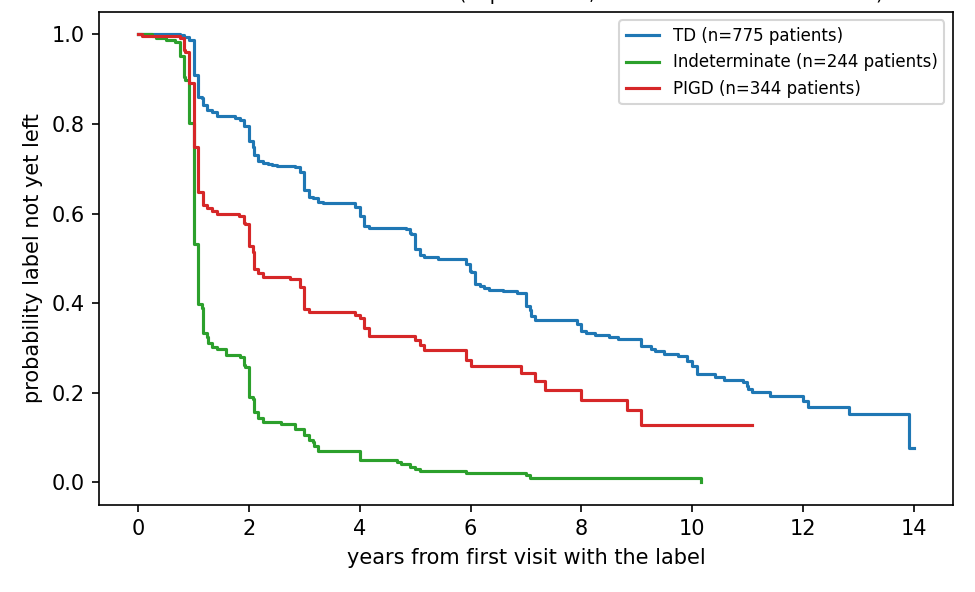
\includegraphics[width=0.80\textwidth]{s02_exit_ind.png}
\caption{Kaplan--Meier time to the first different recorded label, by the label
held at entry, censored at the last labelled visit. The Indeterminate label is
left far faster than either extreme label.}
\label{sfig:exit}
\end{figure}

Figure~\ref{sfig:reversion} gives the reversion rates by type of change that
underlie panel (a) of Table~\ref{tab:dynamics}.

\begin{figure}[htbp]
\centering
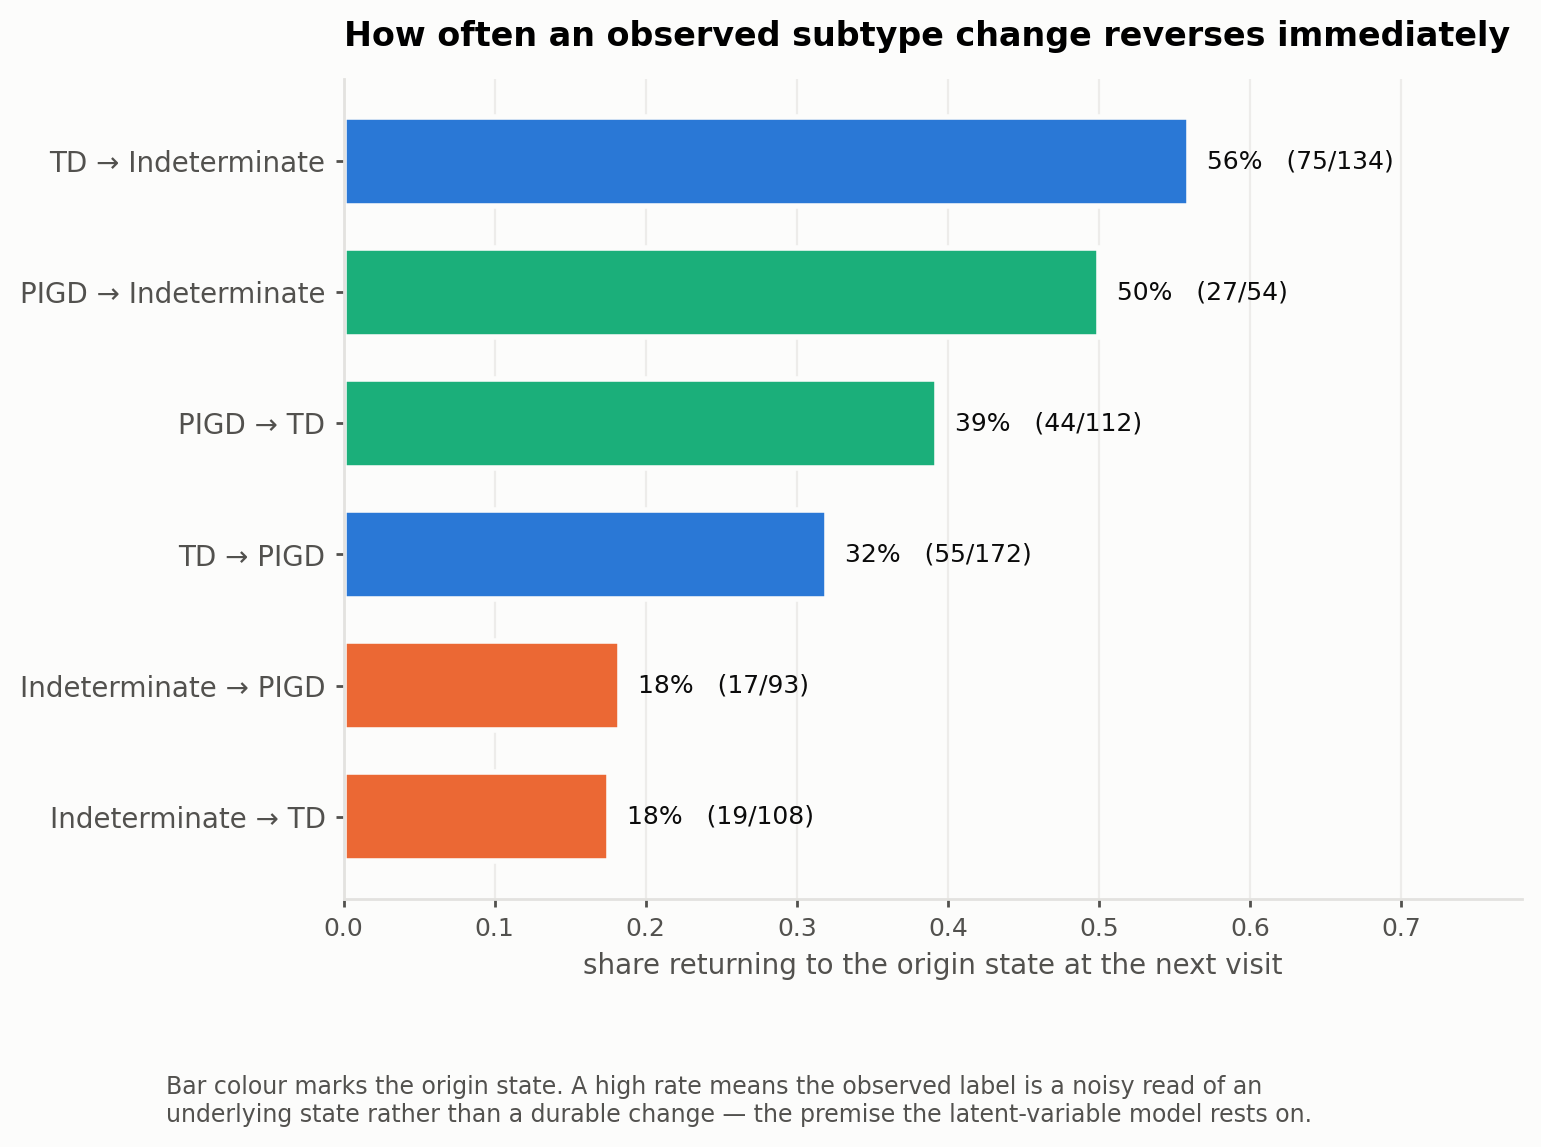
\includegraphics[width=0.80\textwidth]{s01_reversion.png}
\caption{Proportion of observed changes that return to the origin label at the
following visit, by type of change, with patient-clustered bootstrap 95\%
intervals. Changes into the Indeterminate band revert at about half, changes
crossing the full width of the scale at about a third.}
\label{sfig:reversion}
\end{figure}

\paragraph{Limitation.} The clustering statistic has low power at 441
Indeterminate visits, so the inconclusive verdict reflects the design as much as
the data.

% --------------------------------------------------------------------
\section{Localising the generative misfit}
\label{sup:ppc}
% --------------------------------------------------------------------

Section~\ref{sec:ppc} reports that a hierarchical growth model of the ratio with
Student-t slopes and residuals fails a pre-registered posterior-predictive check.
Diagnostics localise the misfit without attaching a verdict.

\paragraph{The Indeterminate excess is a lattice effect.} The excess of 183
Indeterminate visits over the generator's expectation is concentrated at PIGD
item sums 2 (50\% of the excess), 3 (24\%) and 4--5 (22\%); at sum 1 the observed
and expected counts agree (70 against 71.8). Within each stratum the
Indeterminate cells of the lattice hold about as many visits as their
neighbouring cells, so the Indeterminate visits are ordinary lattice points
rather than a local concentration. A band of nominal width 0.25 captures 1.82
times its width in lattice points at PIGD sums 1 and 2; correcting for that
inflation gives an expected share of about 0.068, two thirds of the way from the
observed 0.103 to the generator's 0.051. The whole gap in the ratio distribution
opens inside $(0.90, 1.15]$ and closes again above 2.

\paragraph{The reversion deficit is direction-specific.}
Figure~\ref{sfig:direction} gives the outcome of direct TD--PIGD changes by
direction. TD-to-PIGD changes revert at 0.253 (0.187--0.325) against a generator
expectation of 0.469 --- 37 observed reversions against 83 expected --- whereas
PIGD-to-TD changes revert at 0.398 against an expectation of 0.396. There are
also fewer direct changes overall than the generator implies (244 against 315
with an observed outcome). A symmetric-noise model of a continuous quantity
cannot produce an asymmetry of this kind.

\begin{figure}[htbp]
\centering
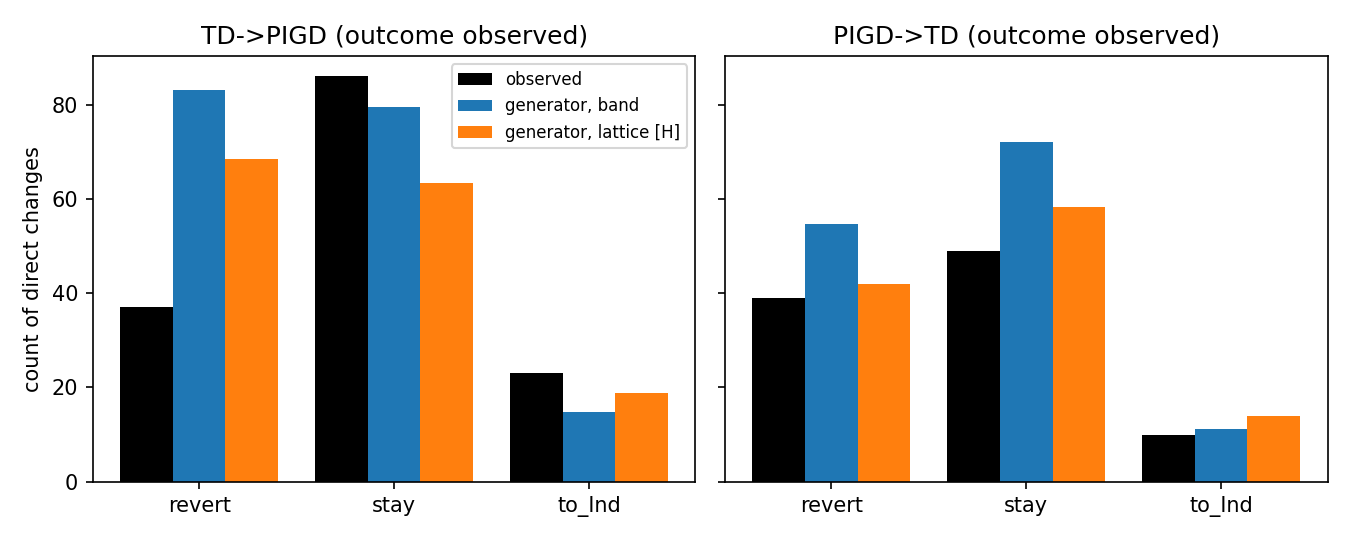
\includegraphics[width=\textwidth]{s03_direction.png}
\caption{Outcome of direct TD--PIGD changes by direction: observed counts against
the expectation under the fitted continuous-ratio generator, treating the band as
a continuous interval and as its lattice catchment. The deficit of observed
reversions is confined to the TD-to-PIGD direction.}
\label{sfig:direction}
\end{figure}

\paragraph{Two caveats.} The diagnostic reference is the covariate-blind generator
rather than the patient-conditional replicate distribution the check itself used,
because the replicate labels were not saved; the re-execution that would have
saved them is described in \ref{sup:notrun}. A valid Student-t residual
diagnostic was not possible from the saved outputs because the fold posteriors of
the random effects were not retained. The misfit is present, and larger, among
the 585 patients with no excluded PIGD-zero visit, which weakens the exclusion of
Section~\ref{sec:undefined} as its driver.

% --------------------------------------------------------------------
\section{Fitted parameters, the emission floor and model stability}
\label{sup:hmm}
% --------------------------------------------------------------------

\subsection{Fitted parameters and the first split}
Table~\ref{stab:hmm} gives the fitted misclassification matrix, the generators
and mean sojourn times of the observed-label and latent chains, and the held-out
performance on the single 70/30 patient split that preceded the
leave-one-patient-out protocol.

Three points follow. The latent generator differs sharply from the observed-label
generator: the latent TD state leaves for PIGD directly at 0.006 per year against
0.058 for the recorded label, and implied mean sojourns are 10.1, 2.1 and 16.5
years in the latent states against 3.4, 0.4 and 2.3 years in the recorded label.
Horizon probabilities computed from the latent generator are latent-to-latent and
\textbf{must not} be read as probabilities of the recorded label: the latent
five-year probability of PIGD given TD is 0.191, whereas the recorded-label chain
gives 0.296.

On the first split the latent-state model reached $-0.638$ log-likelihood per
pair against $-0.665$ for the discrete chain and $-0.675$ for the continuous
chain, and across ten further random splits it beat the discrete chain on every
one, by $+0.028$ per pair on average (SD 0.009). The continuous-time chain
\emph{without} a latent layer loses to the discrete chain at every interval
stratum, because the discrete chain's ``next visit'' absorbs the attendance
schedule that the continuous chain has to model with six rates.

\begin{table}[htbp]
\centering
\caption{Fitted parameters of the three-state hidden Markov model and held-out
performance on the first 70/30 patient split.}
\label{stab:hmm}
\small
\begin{tabular}{@{}lrrr@{}}
\toprule
\multicolumn{4}{@{}l}{\textit{(a) Fitted misclassification matrix $E$ (rows: latent state)}}\\
Latent state & $\Pr(Y{=}\TD)$ & $\Pr(Y{=}\Ind)$ & $\Pr(Y{=}\PIGD)$ \\
\midrule
TD            & 0.9412 & 0.0383 & 0.0205 \\
Indeterminate & 0.2500 & \textbf{0.5000} & 0.2500 \\
PIGD          & 0.1056 & 0.0520 & 0.8424 \\
\midrule
\multicolumn{4}{@{}l}{\textit{(b) Off-diagonal rates (per year) and mean sojourn times (years)}}\\
Quantity & \multicolumn{1}{c}{Observed-label chain} & \multicolumn{2}{c}{Latent chain} \\
\midrule
TD $\to$ Indeterminate            & 0.2348 & \multicolumn{2}{r}{0.0937} \\
TD $\to$ PIGD                     & 0.0583 & \multicolumn{2}{r}{0.0057} \\
Indeterminate $\to$ TD            & 1.2212 & \multicolumn{2}{r}{0.1156} \\
Indeterminate $\to$ PIGD          & 1.0689 & \multicolumn{2}{r}{0.3557} \\
PIGD $\to$ TD                     & 0.0880 & \multicolumn{2}{r}{0.0000} \\
PIGD $\to$ Indeterminate          & 0.3499 & \multicolumn{2}{r}{0.0605} \\
\addlinespace[2pt]
Mean sojourn, TD                  & 3.41 & \multicolumn{2}{r}{10.06} \\
Mean sojourn, Indeterminate       & 0.44 & \multicolumn{2}{r}{2.12} \\
Mean sojourn, PIGD                & 2.28 & \multicolumn{2}{r}{16.52} \\
\midrule
\multicolumn{4}{@{}l}{\textit{(c) Held-out performance on the 70/30 split (1,002 pairs)}}\\
Model & Log-lik.\ / pair & Accuracy & Brier \\
\midrule
Hidden Markov model               & $-0.6384$ & 0.7695 & 0.3458 \\
Markov chain, discrete-time       & $-0.6653$ & 0.7675 & 0.3625 \\
Markov chain, continuous-time     & $-0.6752$ & 0.7655 & 0.3670 \\
Marginal null                     & $-0.8633$ & 0.6248 & 0.5185 \\
\multicolumn{4}{@{}l}{Across ten further splits: HMM $-$ discrete chain $= +0.0284$ (SD 0.0094), positive in 10 of 10.}\\
\bottomrule
\end{tabular}

\end{table}

\begin{figure}[htbp]
\centering
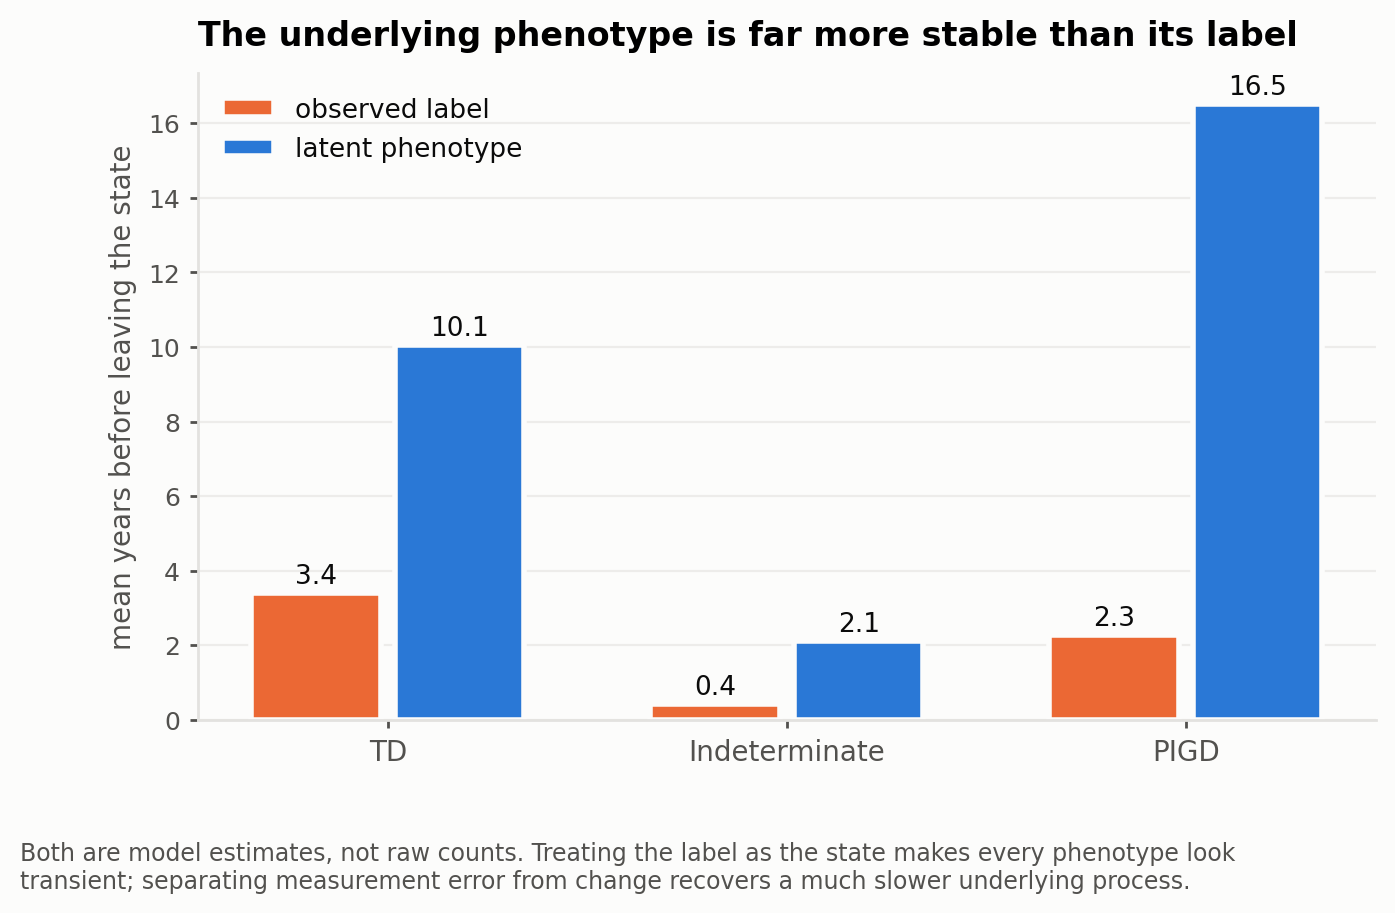
\includegraphics[width=0.80\textwidth]{s04_sojourn.png}
\caption{Mean sojourn times implied by the chain in the recorded label and by the
latent chain of the hidden Markov model. The latent states are far more
persistent than the labels that read them, which is the model's account of the
label's instability.}
\label{sfig:sojourn}
\end{figure}

\subsection{Is the optimum unique, and do more states help?}
Table~\ref{stab:stability} reports 40 random restarts per configuration on the
full cohort and the held-out performance of each configuration.

The three-state floor-constrained fit has a \emph{unique} optimum: all 40 starts
reach the same log-likelihood to within 0.01, with generator entries agreeing to
0.0014 and emission entries to 0.0003. Without the floor the three-state fit sits
on a ridge --- 38 of 40 starts are within 0.01 of the best, yet their emission
entries differ by up to 0.93 --- and the five-state fit is multimodal, with one
of 40 starts within 0.01 of the best and 36 distinct optima at that resolution.

On held-out prediction every configuration is equivalent: accuracies between
0.752 and 0.755 and log-likelihoods between $-0.669$ and $-0.675$. A nested
selection procedure that chose the unconstrained three-state model in eight outer
folds and the five-state model in two reaches 0.755, the same as the audited
model. \textbf{The floor therefore buys identifiability, not accuracy.}

A prior-corrected decision rule that divides each predicted probability by its
class prevalence recovers Indeterminate recall of 0.25 to 0.32 at the cost of
accuracy, which falls to 0.68--0.71. The predicted probabilities themselves do
not change, which locates the failure to predict the minority class in the
interaction between the argmax rule and a rare class, not in the fitted model.

\begin{table}[htbp]
\centering
\caption{Stability of the fitted optimum across random restarts, and held-out
performance of alternative configurations under the argmax rule and under a
prior-corrected rule.}
\label{stab:stability}
\small
\begin{tabular}{@{}lrrrrrr@{}}
\toprule
\multicolumn{7}{@{}l}{\textit{(a) Full-cohort fits from 40 random starts per configuration}}\\
Configuration & Par. & Best log-lik. & Worst log-lik. & Within 0.01 & Optima & Max $|\Delta E|$ \\
\midrule
3 states, floor 0.5 & 14 & $-2969.06$ & $-2969.06$ & 1.000 & 1  & 0.0003 \\
3 states, floor 0.6 & 14 & $-2974.77$ & $-3657.69$ & 0.975 & 2  & 0.0002 \\
3 states, floor 0.7 & 14 & $-2979.10$ & $-3657.69$ & 0.975 & 2  & 0.0000 \\
3 states, free      & 14 & $-2955.32$ & $-2955.45$ & 0.950 & 2  & \textbf{0.9280} \\
4 states, free      & 23 & $-2947.37$ & $-2954.83$ & 0.600 & 15 & 0.0050 \\
5 states, free      & 34 & $-2938.82$ & $-2953.92$ & \textbf{0.025} & \textbf{36} & 0.0000 \\
\midrule
\multicolumn{7}{@{}l}{\textit{(b) Held-out performance of each configuration (argmax rule)}}\\
Configuration & \multicolumn{2}{l}{Accuracy} & \multicolumn{2}{l}{95\% CI} & Bal.\ acc. & Rec.\ Ind. \\
\midrule
3 states, floor 0.5 & \multicolumn{2}{l}{0.7542} & \multicolumn{2}{l}{(0.7351, 0.7734)} & 0.5259 & 0.000 \\
3 states, free      & \multicolumn{2}{l}{0.7539} & \multicolumn{2}{l}{(0.7341, 0.7733)} & 0.5222 & 0.000 \\
4 states, free      & \multicolumn{2}{l}{0.7525} & \multicolumn{2}{l}{(0.7327, 0.7715)} & 0.5222 & 0.000 \\
5 states, free      & \multicolumn{2}{l}{0.7542} & \multicolumn{2}{l}{(0.7348, 0.7732)} & 0.5256 & 0.000 \\
\midrule
\multicolumn{7}{@{}l}{\textit{(c) A prior-corrected decision rule recovers the minority class at a cost}}\\
3 states, floor 0.5 & \multicolumn{2}{l}{0.7123} & \multicolumn{2}{l}{(0.6912, 0.7342)} & 0.5706 & \textbf{0.253} \\
3 states, free      & \multicolumn{2}{l}{0.6897} & \multicolumn{2}{l}{(0.6662, 0.7139)} & 0.5709 & 0.307 \\
5 states, free      & \multicolumn{2}{l}{0.6807} & \multicolumn{2}{l}{(0.6558, 0.7065)} & 0.5702 & 0.319 \\
\bottomrule
\end{tabular}

\end{table}

\subsection{The five-state leave-one-patient-out run}
The five-state specification re-scored in the harmonised comparison reached
0.7513, below the three-state model. Its fits converged in only 404 of 934 folds,
so 59.2\% of its predictions come from non-converged fits. It is reported as a
negative result about model capacity and is not used to support any other claim.

\begin{figure}[htbp]
\centering
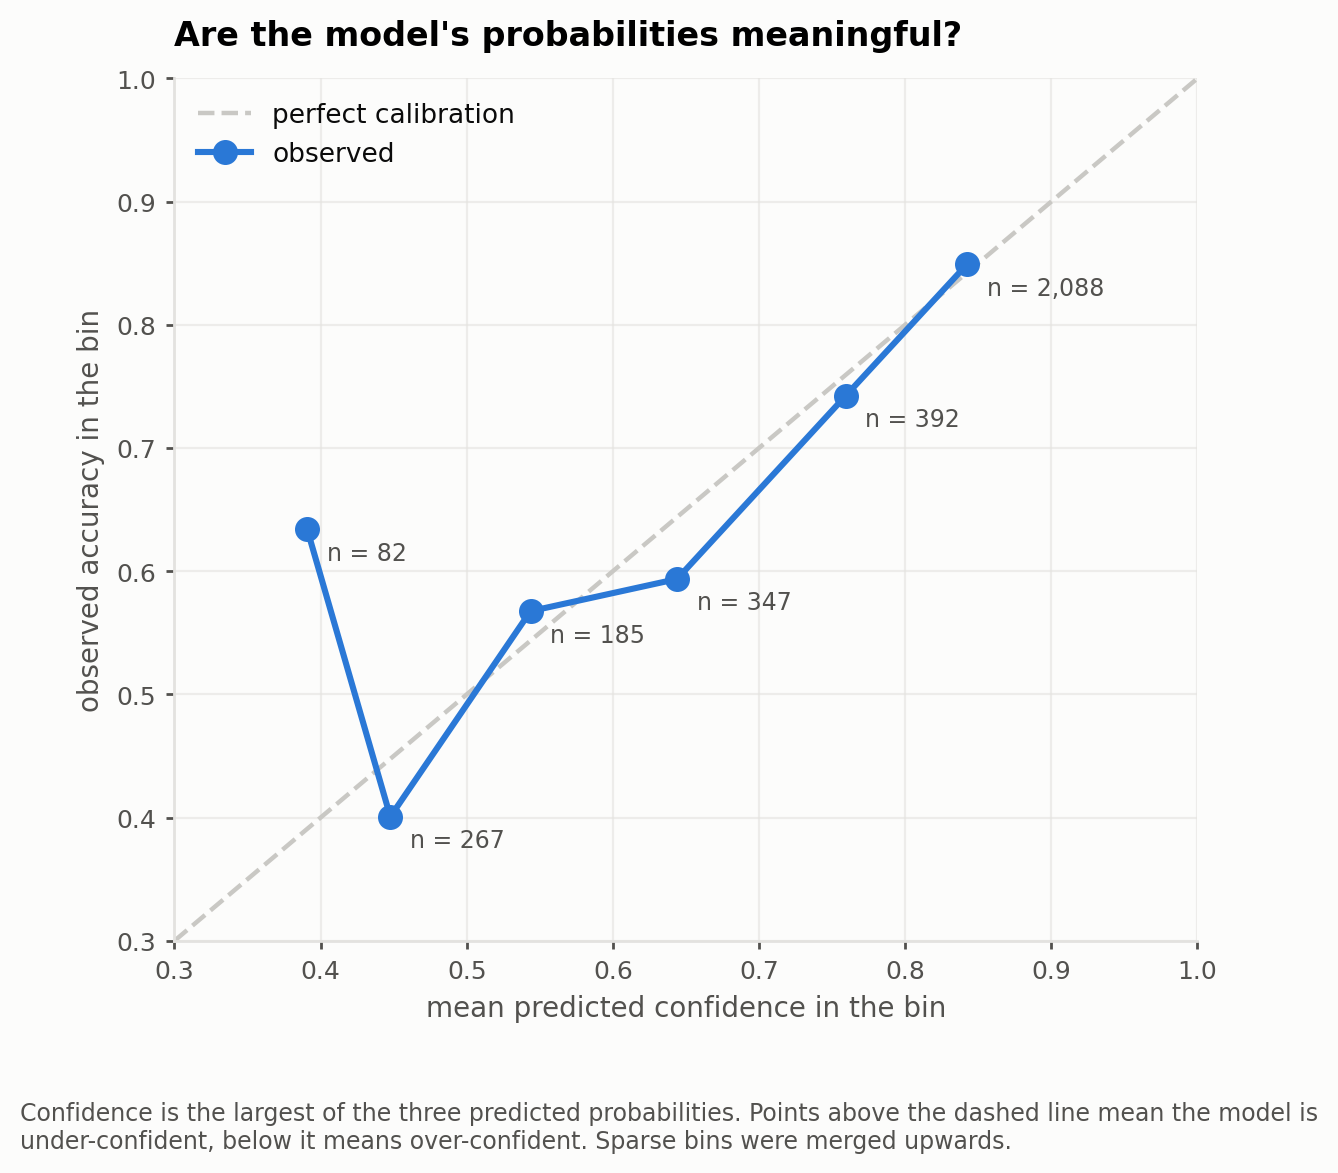
\includegraphics[width=0.74\textwidth]{s05_calibration.png}
\caption{Calibration of the hidden Markov model's maximum predicted probability
under leave-one-patient-out. The reliability curve is close to the diagonal at
the confidence levels the model actually uses.}
\label{sfig:calib}
\end{figure}

% --------------------------------------------------------------------
\section{Prediction with no history}
\label{sup:firstvisit}
% --------------------------------------------------------------------

What can be predicted at a patient's first visit, before any longitudinal
information exists, bounds what the longitudinal models add.

Averaged over ten random 70/30 splits (Table~\ref{stab:firstvisit}), a lookup of
the current label and the prediction horizon gives $-0.781$ log-likelihood per
prediction; adding the baseline ratio gives $-0.773$, adding ten baseline
clinical measures $-0.763$, and both $-0.755$, against $-0.787$ for the hidden
Markov model given no history --- a gain of 0.032 per prediction for the full
first-visit model.

The MDS-UPDRS Part II total is the only covariate whose removal costs more than
0.01 per prediction. DaTscan putamen binding, age and Hoehn \& Yahr stage cost
0.005, 0.004 and 0.002, and the cognitive, olfactory, autonomic and sleep
measures cost nothing or less than nothing. \textbf{None of the
diffuse-synucleinopathy markers predicts the motor label.} Accuracy falls with
horizon from 0.776 within 1.5 years to 0.616 beyond 6.5 years.

\begin{table}[htbp]
\centering
\caption{First-visit prediction with no longitudinal history.}
\label{stab:firstvisit}
\small
\begin{tabular}{@{}lrr@{}}
\toprule
\multicolumn{3}{@{}l}{\textit{(a) Nested first-visit models: held-out log-likelihood per prediction (mean of 10 splits)}}\\
Model & Mean & SD across splits \\
\midrule
Hidden Markov model, no history       & $-0.7869$ & 0.0246 \\
Current subtype $+$ horizon           & $-0.7813$ & 0.0280 \\
\quad $+$ baseline ratio              & $-0.7735$ & 0.0311 \\
\quad $+$ ten baseline covariates     & $-0.7625$ & 0.0378 \\
\quad $+$ ratio $+$ covariates        & $\mathbf{-0.7550}$ & 0.0416 \\
\midrule
\multicolumn{3}{@{}l}{\textit{(b) Cost of dropping each covariate (log-likelihood per prediction)}}\\
Covariate & \multicolumn{2}{r}{Cost of dropping} \\
\midrule
MDS-UPDRS Part II total               & \multicolumn{2}{r}{0.0153} \\
DaTscan putamen binding, bilateral    & \multicolumn{2}{r}{0.0050} \\
Age                                   & \multicolumn{2}{r}{0.0042} \\
Hoehn \& Yahr stage                   & \multicolumn{2}{r}{0.0021} \\
Sex                                   & \multicolumn{2}{r}{0.0002} \\
MoCA, UPSIT, disease duration, SCOPA-AUT, RBDSQ & \multicolumn{2}{r}{$\leq 0$} \\
\midrule
\multicolumn{3}{@{}l}{\textit{(c) Performance by prediction horizon (main split)}}\\
Horizon & $n$ & Accuracy \\
\midrule
$<1.5$ y        & 241 & 0.7759 \\
1.5--3.5 y      & 358 & 0.7570 \\
3.5--6.5 y      & 218 & 0.6789 \\
$>6.5$ y        & 185 & 0.6162 \\
\bottomrule
\end{tabular}

\end{table}

\paragraph{Limitations.} Covariates are mean-imputed within the training split,
and this model was not run under leave-one-patient-out, so its figures are not
directly comparable with the main text's.

% --------------------------------------------------------------------
\section{Student-t variants of the growth model}
\label{sup:studentt}
% --------------------------------------------------------------------

Four variants of the growth model~\eqref{eq:hb} were compared over seven patient
splits, crossing Gaussian or Student-t patient slopes with Gaussian or Student-t
residuals (Table~\ref{stab:studentt}).

\paragraph{Residual tails: supported.} Replacing Gaussian residuals with Student-t
residuals improves held-out prediction unambiguously --- $+0.112$ log predictive
density per visit ($+0.061$ to $+0.168$) with Gaussian slopes, and $+0.106$
($+0.058$ to $+0.158$) with Student-t slopes, positive in all seven splits --- and
improves the class-label metric by about $+0.038$. The fitted residual degrees of
freedom are about 2.1.

\paragraph{Slope tails: not supported.} The original sampler for the slope degrees
of freedom did not converge ($\hat{R} = 1.018$, effective sample size 248) and the
question was declared inconclusive. A pre-registered reassessment with a collapsed
slice sampler converged ($\hat{R} = 1.004$, effective sample size 937) and found a
full-cohort posterior median of 2.09 (1.48--4.11), but met the per-split decision
criterion in only one of seven splits against a threshold of five. The procedure
was calibrated: zero false flags in 180 null cohorts across three scenarios, and
55 of 60 detections in the positive control. The verdict is \textbf{not
supported}.

\paragraph{Why this matters.} The heavy residual tails are the same phenomenon the
lag-1 residual analysis and the posterior-predictive check see from different
directions: occasional large excursions of the ratio that do not persist to the
next visit. They are a property of the measurement, not of patient-level
heterogeneity in progression rate --- which is exactly what the negative result on
slope tails says.

\begin{table}[htbp]
\centering
\caption{Student-t variants of the growth model over seven patient splits. GG,
GT, TG and TT denote Gaussian or Student-t slopes and residuals respectively.}
\label{stab:studentt}
\small
\begin{tabular}{@{}lllr@{}}
\toprule
Question & Quantity & Estimate (95\% interval) & Splits \\
\midrule
\multicolumn{4}{@{}l}{\textit{(a) Are the residuals heavy-tailed? (Q1)}}\\
 & GT $-$ GG, log predictive density per visit & $+0.1115$ ($+0.0606$, $+0.1676$) & 7/7 \\
 & GT $-$ GG, class-label metric              & $+0.0382$ ($+0.0205$, $+0.0549$) & 7/7 \\
 & TT $-$ TG, log predictive density per visit & $+0.1060$ ($+0.0577$, $+0.1575$) & 7/7 \\
 & TT $-$ TG, class-label metric              & $+0.0379$ ($+0.0212$, $+0.0546$) & 7/7 \\
 & \multicolumn{3}{l}{\textbf{Verdict: supported.} Residual degrees of freedom $\approx 2.1$.} \\
\addlinespace[3pt]
\multicolumn{4}{@{}l}{\textit{(b) Are the patient slopes heavy-tailed? (Q2)}}\\
 & Original run: $\hat{R}$ / effective sample size & 1.018 / 248 & inconclusive \\
 & Reassessment: $\hat{R}$ / effective sample size & 1.0044 / 937 & converged \\
 & Full-cohort posterior median $\nu_{\mathrm{slope}}$ & 2.09 (1.48, 4.11) & --- \\
 & Per-split criterion met ($\nu$ upper bound $<10$) & 1 of 7 & threshold 5/7 \\
 & Null calibration, scenarios C1--C3 & 0 flags in 180 cohorts & --- \\
 & Positive control, scenario P & 55 of 60 detected & --- \\
 & \multicolumn{3}{l}{\textbf{Verdict: not supported.} No evidence of extreme slope tails.} \\
\addlinespace[3pt]
\multicolumn{4}{@{}l}{\textit{(c) Predictive value of each variant against the Gaussian model (Q3)}}\\
 & TG, class-label metric & $+0.0034$ ($+0.0007$, $+0.0063$) & 6/7 \\
 & GT, class-label metric & $+0.0382$ ($+0.0205$, $+0.0549$) & 7/7 \\
 & TT, class-label metric & $+0.0412$ ($+0.0229$, $+0.0586$) & 7/7 \\
\bottomrule
\end{tabular}

\end{table}

% --------------------------------------------------------------------
\section{The full subscore comparison}
\label{sup:subscore}
% --------------------------------------------------------------------

Table~\ref{stab:subscore} gives the fifteen-arm held-out comparison of subscore
models on identical points, the pre-specified paired contrasts, the derived-label
contrasts against the hidden Markov model, and the parameters of the joint
bivariate mixed model.

\paragraph{The cross-output block is worth nothing.} The full coregionalisation
block is indistinguishable from its diagonal counterpart on every metric and both
outcomes: the largest effect is a change of $-0.0002$ in tremor CRPS. The reason
is that the two subscores are nearly uncorrelated, with a random-intercept
correlation of $-0.015$ and a residual correlation of $+0.019$. All 3,736
multi-output fits converged.

\paragraph{Temporal flexibility helps the proper scores, not the absolute error.}
Kernels carrying both a linear term and a flexible component ($K_2$, $K_3$) beat
the simpler ones on CRPS and log score for both outcomes --- joint log score
$+0.073$ ($+0.051$ to $+0.096$) for $K_2$ against $K_0$ --- while MAE moves by
thousandths. Every Gaussian process beats persistence on CRPS and log score, and
loses to it on PIGD absolute error.

\paragraph{The interpretable parametric comparator loses.} The joint bivariate
mixed model estimates population slopes of $+0.023$ per year for tremor and
$+0.066$ for PIGD, with intraclass correlations of 0.61 and 0.45. Its held-out
MAE is worse than persistence on both outcomes ($+0.012$ and $+0.035$), and its
derived label is worse than the hidden Markov model on log loss ($+0.018$,
$+0.004$ to $+0.032$).

\paragraph{The derived label under two rules.} Classifying the point prediction
gives 0.730 accuracy and recovers Indeterminate at recall 0.17; taking the argmax
of the Monte Carlo probability vector gives 0.757 and recovers it at 0.000. The
two rules differ by more than the entire spread between fitted models, which is
why the main text harmonises on one of them (Section~\ref{sec:harmonisation}).

\begin{table}[htbp]
\centering
\caption{The full subscore comparison on identical leave-one-patient-out points.}
\label{stab:subscore}
\footnotesize
\begin{tabular}{@{}llrrrr@{}}
\toprule
Outcome & Model & MAE & CRPS & Log score & Cov.\ 95\% \\
\midrule
\multicolumn{6}{@{}l}{\textit{(a) Fifteen-arm held-out comparison (934 patients, 3,361 points)}}\\
tremor & GP, $K_0$              & 0.2385 & 0.1716 & $-0.2482$ & 0.939 \\
tremor & GP, $K_1$              & 0.2395 & 0.1708 & $-0.2392$ & 0.936 \\
tremor & GP, $K_2$              & 0.2358 & 0.1689 & $-0.2264$ & 0.937 \\
tremor & GP, $K_3$              & 0.2359 & 0.1690 & $-0.2262$ & 0.937 \\
tremor & GP, joint $K_1$ full   & 0.2391 & 0.1706 & $-0.2378$ & 0.936 \\
tremor & Mixed model (RI)       & 0.2546 & 0.1817 & $-0.3151$ & 0.935 \\
tremor & Patient mean           & 0.2498 & 0.1830 & $-0.3158$ & 0.926 \\
tremor & Persistence            & 0.2426 & 0.1797 & $-0.3024$ & 0.953 \\
\addlinespace[2pt]
pigd   & GP, $K_0$              & 0.2156 & 0.1634 & $-0.2848$ & 0.944 \\
pigd   & GP, $K_1$              & 0.2175 & 0.1618 & $-0.2648$ & 0.933 \\
pigd   & GP, $K_2$              & 0.2132 & 0.1601 & $-0.2339$ & 0.939 \\
pigd   & GP, $K_3$              & 0.2129 & 0.1599 & $-0.2334$ & 0.939 \\
pigd   & GP, joint $K_1$ full   & 0.2173 & 0.1617 & $-0.2644$ & 0.933 \\
pigd   & Mixed model (RI)       & 0.2391 & 0.1809 & $-0.4225$ & 0.940 \\
pigd   & Patient mean           & 0.2400 & 0.1985 & $-0.5281$ & 0.932 \\
pigd   & Persistence            & \textbf{0.2040} & 0.1724 & $-0.3486$ & 0.951 \\
\midrule
\multicolumn{6}{@{}l}{\textit{(b) Pre-specified paired contrasts}}\\
\multicolumn{2}{@{}l}{Cross-output block vs its diagonal ($K_1$, tremor, CRPS)}
   & \multicolumn{4}{l}{$-0.0002$ ($-0.0003$, $+0.0000$) \quad neither} \\
\multicolumn{2}{@{}l}{Temporal flexibility, $K_2 - K_0$ (joint log score)}
   & \multicolumn{4}{l}{$+0.0726$ ($+0.0511$, $+0.0957$) \quad \textbf{model}} \\
\multicolumn{2}{@{}l}{$K_1 -$ persistence (joint log score)}
   & \multicolumn{4}{l}{$+0.1437$ ($+0.1020$, $+0.1860$) \quad \textbf{model}} \\
\midrule
\multicolumn{6}{@{}l}{\textit{(c) Derived three-class label vs the hidden Markov model on the same 3,361 points}}\\
\multicolumn{2}{@{}l}{GP $K_1$, accuracy (argmax)} & \multicolumn{4}{l}{$+0.0024$ ($-0.0045$, $+0.0092$)} \\
\multicolumn{2}{@{}l}{GP joint $K_1$, accuracy (argmax)} & \multicolumn{4}{l}{$+0.0045$ ($-0.0026$, $+0.0117$)} \\
\multicolumn{2}{@{}l}{GP $K_1$, log loss} & \multicolumn{4}{l}{$-0.0196$ ($-0.0317$, $-0.0073$) \quad \textbf{favours the GP}} \\
\multicolumn{2}{@{}l}{Mixed model, log loss} & \multicolumn{4}{l}{$+0.0177$ ($+0.0035$, $+0.0324$) \quad \textbf{favours the HMM}} \\
\midrule
\multicolumn{6}{@{}l}{\textit{(d) Joint bivariate mixed model: fixed effects (934 patients, 8,590 observations)}}\\
\multicolumn{2}{@{}l}{Tremor intercept / slope per year}
   & \multicolumn{4}{l}{0.5841 (0.5594, 0.6089) \,/\, $+0.0233$ ($+0.0202$, $+0.0265$)} \\
\multicolumn{2}{@{}l}{PIGD intercept / slope per year}
   & \multicolumn{4}{l}{0.2301 (0.2085, 0.2517) \,/\, $+0.0655$ ($+0.0621$, $+0.0689$)} \\
\multicolumn{2}{@{}l}{Random-intercept / residual correlation}
   & \multicolumn{4}{l}{$-0.0153$ \,/\, $+0.0186$} \\
\multicolumn{2}{@{}l}{Intraclass correlation, tremor / PIGD}
   & \multicolumn{4}{l}{0.6067 \,/\, 0.4527} \\
\bottomrule
\end{tabular}

\end{table}

\paragraph{Limitations.} Raw-scale Gaussian likelihoods on bounded, zero-inflated
scores; the derived label uses Monte Carlo through a ratio of two Gaussians
clipped at zero; the subscore models train on 934 patients and the ratio model on
821, so their absolute errors are not comparable with each other.

% --------------------------------------------------------------------
\section{Time-varying rates and their identifiability}
\label{sup:temporal}
% --------------------------------------------------------------------

Table~\ref{stab:temporal} reports the period-specific slopes of the two subscores
under a linear-spline mixed model, the within-patient change in rate, a dedicated
identifiability audit, and an attrition model.

\paragraph{The population pattern is clear.} The PIGD slope rises across follow-up
(0.045, 0.057 and 0.080 per year in years 0--2, 2--5 and beyond 5) and the tremor
slope falls (0.033, 0.033 and 0.013). The contrasts between the last and the first
period are $+0.035$ for PIGD and $-0.020$ for tremor, and within the 226 patients
observed in both periods the PIGD rate rises by $+0.073$ ($+0.043$ to $+0.101$)
and the tremor rate falls by $-0.040$ ($-0.073$ to $-0.008$). So the pattern is
within patients as well as between them (Figure~\ref{sfig:slopes}).

\paragraph{But it is not identifiable, not honest, and not predictive.} A
supremum likelihood-ratio test confirms a departure from linearity (39.1 against
a bootstrap 95th percentile of 7.7 under a random-intercept null and 20.4 under a
random-slope null, $P = 0.005$ under both), but the best single knot sits at 4.75
years with a bootstrap range of 2.5 to 10 years, and a quadratic mean is preferred
by AIC over a linear one by 37.8 units. The Wald intervals on the late-period
slopes are too narrow by factors of 1.7 (tremor) and 2.2 (PIGD) against a patient
bootstrap. Attrition is informative: the log-odds of loss to follow-up after a
visit rise by $+0.52$ ($+0.36$ to $+0.71$) per point of PIGD score. On a
disease-duration time axis the slope changes at five years no longer exclude zero,
and the treated share rises from 0.10 at baseline to 0.95 by year five, so the
acceleration is confounded with duration and treatment.

Held out, the spline improves PIGD absolute error over the constant-rate model by
$-0.0034$ ($-0.0044$ to $-0.0023$) and tremor not at all, and both lose to
persistence; the derived label is 0.709 under either. \textbf{This is a population
description, not a predictive feature}, and it is why no time-varying structure
enters the prediction models of the main text.

\begin{table}[htbp]
\centering
\caption{Time-varying rates of the two subscores, and the audit of their
identifiability and interval coverage.}
\label{stab:temporal}
\small
\begin{tabular}{@{}llrll@{}}
\toprule
Outcome & Period & Slope / y & Wald 95\% CI & Patient-bootstrap 95\% CI \\
\midrule
\multicolumn{5}{@{}l}{\textit{(a) Period-specific population slopes (knots at 2 and 5 years)}}\\
tremor & 0--2 y  & 0.0327 & (0.0196, 0.0458) & (0.0201, 0.0450) \\
tremor & 2--5 y  & 0.0325 & (0.0212, 0.0439) & (0.0189, 0.0458) \\
tremor & $>$5 y  & 0.0126 & (0.0056, 0.0197) & (0.0001, 0.0238) \\
pigd   & 0--2 y  & 0.0450 & (0.0309, 0.0592) & (0.0348, 0.0564) \\
pigd   & 2--5 y  & 0.0574 & (0.0453, 0.0695) & (0.0429, 0.0733) \\
pigd   & $>$5 y  & 0.0800 & (0.0724, 0.0875) & (0.0640, 0.0971) \\
\addlinespace[2pt]
\multicolumn{5}{@{}l}{SE ratio, bootstrap / Wald, late period: tremor 1.72, PIGD 2.23.}\\
\midrule
\multicolumn{5}{@{}l}{\textit{(b) Within-patient change in rate (patients observed in both periods)}}\\
pigd   & 0--2 $\to$ $>$5 y & $+0.0727$ & \multicolumn{2}{l}{($+0.0425$, $+0.1014$), $n = 226$} \\
tremor & 0--2 $\to$ $>$5 y & $-0.0396$ & \multicolumn{2}{l}{($-0.0731$, $-0.0079$), $n = 226$} \\
\midrule
\multicolumn{5}{@{}l}{\textit{(c) Is the change in rate identifiable?}}\\
\multicolumn{2}{@{}l}{Supremum likelihood ratio} & 39.13 & \multicolumn{2}{l}{$P = 0.005$ under both null models} \\
\multicolumn{2}{@{}l}{Null 95th percentile} & 7.68 / 20.39 & \multicolumn{2}{l}{random-intercept / random-slope null} \\
\multicolumn{2}{@{}l}{Best single knot} & 4.75 y & \multicolumn{2}{l}{bootstrap 2.5--97.5 pct: 2.5 to 10 y} \\
\multicolumn{2}{@{}l}{Held-out gain over a linear trend} & \multicolumn{3}{l}{PIGD MAE $-0.0034$; tremor none; both lose to persistence} \\
\midrule
\multicolumn{5}{@{}l}{\textit{(d) Attrition after a visit (logistic, bootstrap intervals)}}\\
\multicolumn{2}{@{}l}{Years from baseline} & $+0.1386$ & \multicolumn{2}{l}{($+0.1221$, $+0.1576$)} \\
\multicolumn{2}{@{}l}{PIGD subscore} & $+0.5206$ & \multicolumn{2}{l}{($+0.3598$, $+0.7137$)} \\
\multicolumn{2}{@{}l}{Tremor subscore} & $+0.0024$ & \multicolumn{2}{l}{($-0.1535$, $+0.1521$)} \\
\bottomrule
\end{tabular}

\end{table}

\begin{figure}[htbp]
\centering
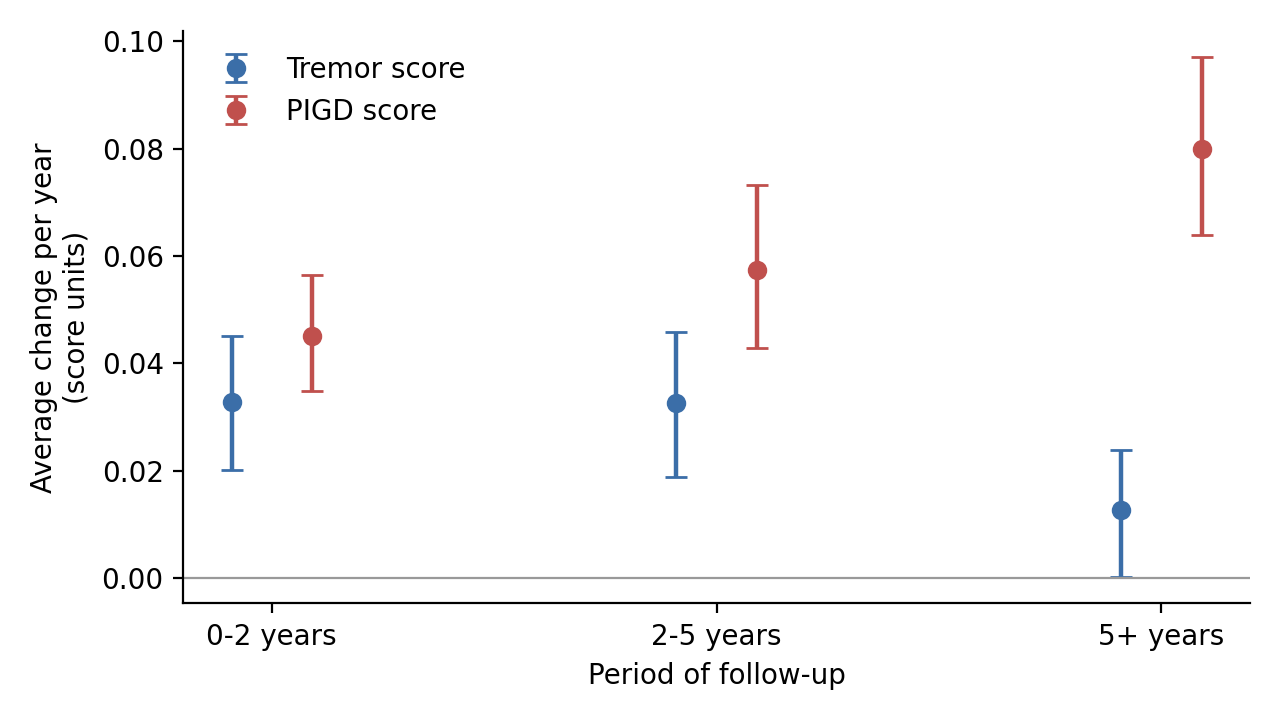
\includegraphics[width=0.84\textwidth]{s06_slopes.png}
\caption{Period-specific population slopes of the tremor and PIGD subscores under
the linear-spline mixed model. The PIGD rate accelerates and the tremor rate
decelerates over follow-up; the Wald intervals shown are too narrow by factors of
1.7 and 2.2 against a patient bootstrap.}
\label{sfig:slopes}
\end{figure}

% --------------------------------------------------------------------
\section{Discrete latent clinical states}
\label{sup:clinical}
% --------------------------------------------------------------------

Section~\ref{sec:richer} reports that a discrete latent state over ten clinical
measurements predicts the next label substantially \emph{worse} than the subtype
history alone. Table~\ref{stab:clinical} gives the full comparison.

State count was selected on a 280-patient development set by held-out next-visit
log-density, which improves monotonically from two to eight states; six states
were chosen by the one-standard-error rule and eight by the maximum. The fits are
multimodal from four states upward, with the spread of the training
log-likelihood across random starts exceeding 1,000 nats.

On 2,091 identical two-class cases the six-state model reaches 0.7255 and the
eight-state model 0.7336, against 0.8384 for the subtype-history model: paired
differences of $-0.1130$ and $-0.1048$, both intervals excluding zero. The loss is
concentrated where the current label is PIGD, with accuracy 0.397 against 0.787
and PIGD recall 0.218 against 0.659.

The bottleneck, not the measurements, is responsible. A direct logistic model on
the same ten measurements and the interval reaches 0.8307 with the \emph{best}
Brier score and log loss of any model on that evaluation set --- $+0.1052$ over
the latent model, and indistinguishable from the subtype-history model
($-0.0077$, $-0.0204$ to $+0.0046$). Restricting it to the tremor and PIGD scores
alone changes nothing ($-0.0010$, $-0.0114$ to $+0.0091$), so eight of the ten
measurements add nothing to this target.

\paragraph{Interpretation.} Forcing ten continuous measurements through a handful
of discrete states orders patients by overall severity and discards the
within-patient variation the prediction needs. This experiment is the reason the
programme replaced the discrete state with the continuous per-domain profile of
Section~\ref{sec:richer}.

\begin{table}[htbp]
\centering
\caption{Discrete latent clinical states against the subtype history and against
direct models on the same measurements. $^{\dagger}$The persistence rule's log
loss is reported clipped.}
\label{stab:clinical}
\footnotesize
\setlength{\tabcolsep}{4pt}
\begin{tabular}{@{}lrlrr@{}}
\toprule
Model & Accuracy & 95\% CI & Brier & Log loss \\
\midrule
\multicolumn{5}{@{}l}{\textit{Identical 2,091 two-class cases, 627 patients with cases}}\\
Subtype-history hidden Markov model (labels only) & \textbf{0.8384} & (0.8183, 0.8568) & 0.1211 & 0.3953 \\
Persistence (last non-Indeterminate label)        & 0.8350 & (0.8147, 0.8541) & 0.1590 & $4.173^{\dagger}$ \\
Direct logistic on the ten measurements           & 0.8307 & (0.8086, 0.8515) & \textbf{0.1156} & \textbf{0.3646} \\
Direct logistic on tremor and PIGD scores only    & 0.8297 & (0.8080, 0.8495) & 0.1202 & 0.3819 \\
Latent clinical-state HMM, 6 states               & 0.7255 & (0.6960, 0.7534) & 0.1831 & 0.5493 \\
Latent clinical-state HMM, 8 states               & 0.7336 & (0.7062, 0.7607) & 0.1817 & 0.5444 \\
\midrule
\multicolumn{5}{@{}l}{\textit{Paired contrasts}}\\
\multicolumn{2}{@{}l}{Latent clinical state (6) $-$ subtype-history HMM}
   & \multicolumn{3}{l}{$-0.1130$ ($-0.1438$, $-0.0807$) \quad \textbf{excludes zero}} \\
\multicolumn{2}{@{}l}{Latent clinical state (8) $-$ subtype-history HMM}
   & \multicolumn{3}{l}{$-0.1048$ ($-0.1357$, $-0.0757$) \quad \textbf{excludes zero}} \\
\multicolumn{2}{@{}l}{Same measurements, no latent bottleneck}
   & \multicolumn{3}{l}{$+0.1052$ ($+0.0756$, $+0.1338$) \quad \textbf{excludes zero}} \\
\multicolumn{2}{@{}l}{Ten measurements $-$ subtype history}
   & \multicolumn{3}{l}{$-0.0077$ ($-0.0204$, $+0.0046$)} \\
\multicolumn{2}{@{}l}{Two label-defining scores $-$ all ten}
   & \multicolumn{3}{l}{$-0.0010$ ($-0.0114$, $+0.0091$)} \\
\midrule
\multicolumn{5}{@{}l}{\textit{Where the latent model loses: accuracy by the label recorded at the prediction point}}\\
\multicolumn{2}{@{}l}{Current TD} & \multicolumn{3}{l}{0.844 (latent) vs 0.881 (subtype history)} \\
\multicolumn{2}{@{}l}{Current Indeterminate} & \multicolumn{3}{l}{0.568 vs 0.614} \\
\multicolumn{2}{@{}l}{Current PIGD} & \multicolumn{3}{l}{\textbf{0.397} vs 0.787} \\
\bottomrule
\end{tabular}

\end{table}

\paragraph{Limitation.} The evaluation set is a 654-patient subset, so absolute
numbers differ from the 899-patient runs elsewhere in the paper; only the paired
contrasts on identical cases should be read across.

% --------------------------------------------------------------------
\section{Information criteria, boundary calls and dimensionality}
\label{sup:misc}
% --------------------------------------------------------------------

Table~\ref{stab:misc} collects three supporting analyses.

\paragraph{(a) Information criteria.} Among models sharing a joint sequence
likelihood, the hidden Markov model is preferred over a discrete chain with an
initial distribution by 224 AIC units and 186 BIC units, and over the continuous
chain by 250 AIC units. Among the chains alone the discrete chain is preferred
over the continuous one by 25 units. Among profile variants the full model is
preferred over the level-only variant by 221 AIC and 67 BIC units. \textbf{The
three groups are not mutually comparable} --- the chains' conditional pair
likelihood, the joint sequence likelihood and the profile's continuous density
are different objects --- and these criteria are in-sample and assume independent
observations, so they favour the latent layer more than clustered data warrant.

\paragraph{(b) Calls at Indeterminate visits.} At the 287 Indeterminate visits
with a defined ratio, does a model call the side of the band the ratio sits
nearer? The hidden Markov model agrees with the nearer boundary at 0.488 against
0.462 expected under independence, an excess of $+0.026$ ($-0.029$ to $+0.078$);
the profile at 0.502 against 0.471, an excess of $+0.031$ ($-0.022$ to $+0.088$).
Both intervals contain zero, as does the sensitivity analysis restricted to the
213 visits closest to a boundary. The models' \emph{probabilities} lean towards
the nearer side --- AUC 0.584 and 0.575 for ranking nearer-PIGD visits --- but
their \emph{calls} barely do. This is the same accuracy-versus-ranking
dissociation reported in the main text, seen at the one stratum that matters most.

\paragraph{(c) Dimensionality of the profile.} Seven of nine principal components
are required for 90\% of the across-patient variance of either the level or the
rate coordinates, with the first carrying 42\% and 37\% respectively and
participation-ratio effective ranks of 4.3 and 5.1
(Figure~\ref{sfig:dim}). The representation is therefore genuinely
multidimensional and not a severity score in disguise.

\begin{table}[htbp]
\centering
\caption{Information criteria, model calls at Indeterminate visits, and the
dimensionality of the nine-domain representation.}
\label{stab:misc}
\small
\setlength{\tabcolsep}{5pt}
\begin{tabular}{@{}llrr@{}}
\toprule
\multicolumn{4}{@{}l}{\textit{(a) Information criteria; groups are comparable only within themselves}}\\
Group & Model & $\Delta$AIC & $\Delta$BIC \\
\midrule
Joint sequence likelihood & Hidden Markov model (3 latent states) & 0.0 & 0.0 \\
                          & Discrete chain $+$ initial state      & 224.1 & 185.9 \\
                          & Continuous chain $+$ initial state    & 249.6 & 211.4 \\
\addlinespace[2pt]
Conditional pair likelihood & Markov chain, discrete-time         & 0.0 & 0.0 \\
                            & Markov chain, continuous-time       & 25.5 & 25.5 \\
\addlinespace[2pt]
Rich-profile variants     & Level $+$ rate $+$ medication         & 0.0 & 0.0 \\
                          & Level only (random walk)              & 220.8 & 66.8 \\
                          & Level $+$ rate, no medication         & 344.0 & 266.9 \\
\midrule
\multicolumn{4}{@{}l}{\textit{(b) Calls at the 287 Indeterminate visits with a defined ratio (220 patients)}}\\
Quantity & Model & \multicolumn{2}{l}{Estimate (95\% CI)} \\
\midrule
Agreement with nearer boundary & Hidden Markov model & \multicolumn{2}{l}{0.488 (0.434, 0.540)} \\
                               & Rich clinical profile & \multicolumn{2}{l}{0.502 (0.448, 0.559)} \\
Expected under independence    & Hidden Markov model & \multicolumn{2}{l}{0.462} \\
                               & Rich clinical profile & \multicolumn{2}{l}{0.471} \\
Excess over independence       & Hidden Markov model & \multicolumn{2}{l}{$+0.026$ ($-0.029$, $+0.078$)} \\
                               & Rich clinical profile & \multicolumn{2}{l}{$+0.031$ ($-0.022$, $+0.088$)} \\
\quad sensitivity set ($n{=}213$) & Hidden Markov model & \multicolumn{2}{l}{$+0.038$ ($-0.029$, $+0.103$)} \\
                               & Rich clinical profile & \multicolumn{2}{l}{$+0.062$ ($-0.002$, $+0.127$)} \\
AUC for ranking nearer-PIGD    & Hidden Markov model & \multicolumn{2}{l}{0.584 (0.516, 0.653)} \\
                               & Rich clinical profile & \multicolumn{2}{l}{0.575 (0.505, 0.640)} \\
\midrule
\multicolumn{4}{@{}l}{\textit{(c) Dimensionality of the nine-domain representation (934 patients)}}\\
Quantity & & Level & Rate \\
\midrule
First principal component, variance share & & 42.2\% & 37.2\% \\
First three components, cumulative        & & 66.3\% & 60.2\% \\
Components needed for 90\%                & & 7 of 9 & 7 of 9 \\
Participation-ratio effective rank        & & 4.34 & 5.11 \\
\bottomrule
\end{tabular}

\end{table}

\begin{figure}[htbp]
\centering
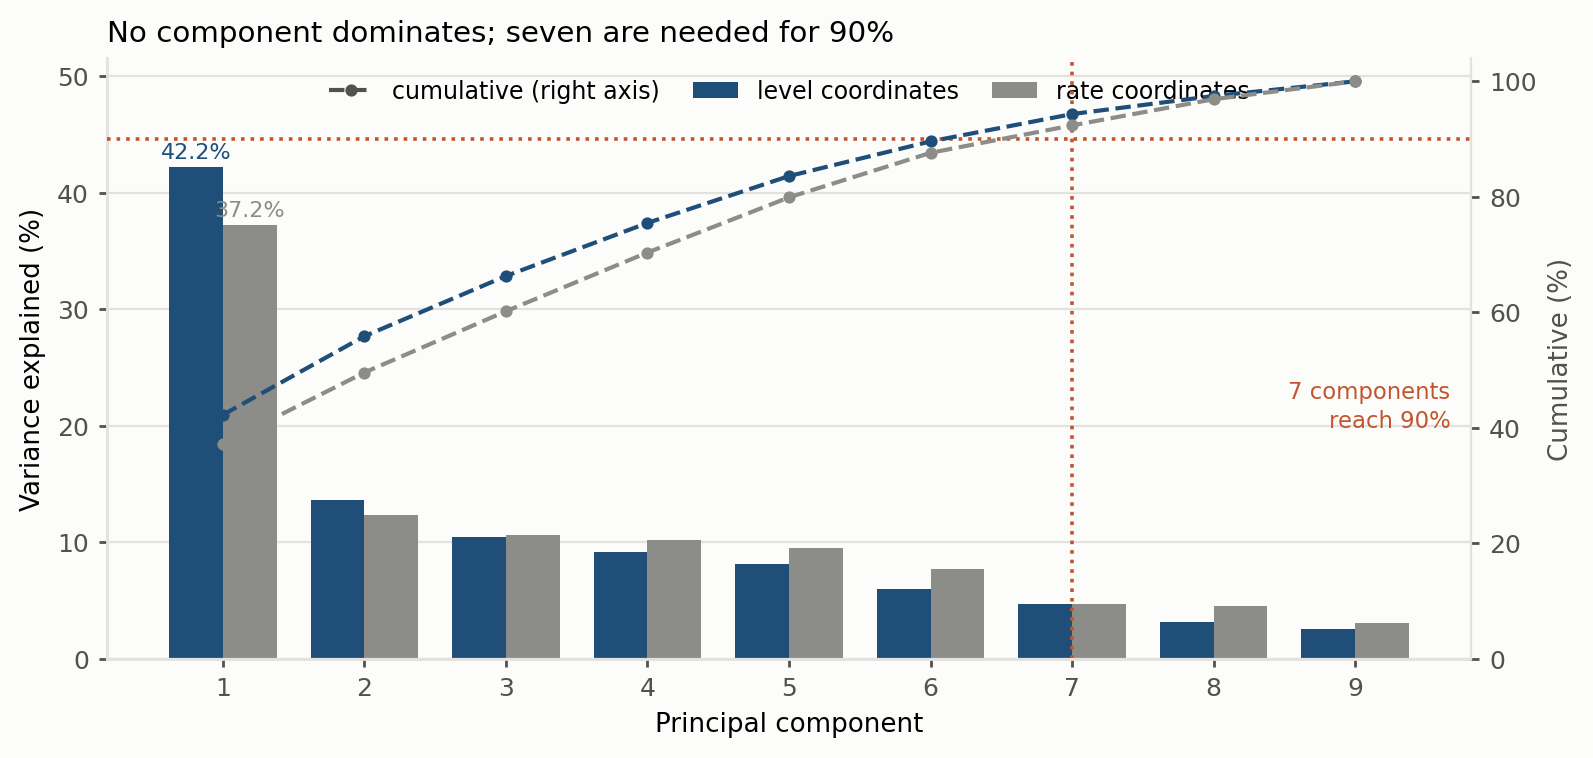
\includegraphics[width=0.74\textwidth]{s11_dimensionality.png}
\caption{Cumulative share of across-patient variance explained by successive
principal components of the profile's level and rate coordinates. Seven of nine
components are needed for 90\% of either.}
\label{sfig:dim}
\end{figure}

% --------------------------------------------------------------------
\section{Accuracy by prediction stage}
\label{sup:stage}
% --------------------------------------------------------------------

Does prediction get easier as a patient accumulates visits?
Table~\ref{stab:stage} reports two-class metrics at each prediction stage, where
stage $k$ predicts visit $k+1$ from visits $1 \dots k$, for the nine stages with
at least 66 targets.

\textbf{No change in accuracy from stage 1 excludes zero} for either model at any
reliable stage, and of 24 pre-specified paired tests exactly one interval excludes
zero: the profile's balanced accuracy at stage 1, $+0.046$ ($+0.023$ to $+0.070$),
which reflects its better PIGD sensitivity when only one visit is known and does
not persist.

Balanced accuracy does rise with stage for every model --- including the
persistence rule, from 0.717 at stage 1 to 0.816 at stage 9 --- but so does the
PIGD share of outcomes, from 23\% to 48\%. The trend is cohort composition, not
learning. Within the 225 patients observed at both early and late stages, the
late-minus-early change in accuracy is $-0.024$ ($-0.075$ to $+0.028$) for the
hidden Markov model and $-0.035$ ($-0.089$ to $+0.020$) for the profile.

\begin{table}[htbp]
\centering
\caption{Two-class metrics by prediction stage (3,017 targets of 896 patients).}
\label{stab:stage}
\small
\begin{tabular}{@{}rrrrrrr@{}}
\toprule
Stage & $n$ targets & \% PIGD & HMM acc. & Profile acc. & Persist.\ acc. & HMM bal.\ acc. \\
\midrule
1 & 835 & 23.5 & 0.8347 & 0.8455 & 0.8323 & 0.7293 \\
2 & 693 & 26.0 & 0.8644 & 0.8644 & 0.8600 & 0.8110 \\
3 & 450 & 29.3 & 0.8267 & 0.8200 & 0.8289 & 0.7799 \\
4 & 305 & 31.8 & 0.8098 & 0.8230 & 0.8033 & 0.7698 \\
5 & 200 & 34.0 & 0.8200 & 0.8350 & 0.8250 & 0.7888 \\
6 & 171 & 40.9 & 0.8304 & 0.8129 & 0.8187 & 0.8148 \\
7 & 125 & 40.0 & 0.8400 & 0.8240 & 0.8240 & 0.8200 \\
8 & 93  & 46.2 & 0.8495 & 0.8387 & 0.8602 & 0.8453 \\
9 & 66  & 48.5 & 0.8485 & 0.8485 & 0.8182 & 0.8474 \\
\midrule
\multicolumn{7}{@{}l}{Of 24 pre-specified paired tests, one interval excludes zero: the profile's balanced accuracy}\\
\multicolumn{7}{@{}l}{at stage 1, $+0.046$ ($+0.023$, $+0.070$). No change in accuracy from stage 1 excludes zero for}\\
\multicolumn{7}{@{}l}{either model at any reliable stage. Within-patient late $-$ early change in accuracy: hidden Markov}\\
\multicolumn{7}{@{}l}{model $-0.024$ ($-0.075$, $+0.028$); profile $-0.035$ ($-0.089$, $+0.020$); $n = 225$ patients.}\\
\bottomrule
\end{tabular}

\end{table}

\begin{figure}[htbp]
\centering
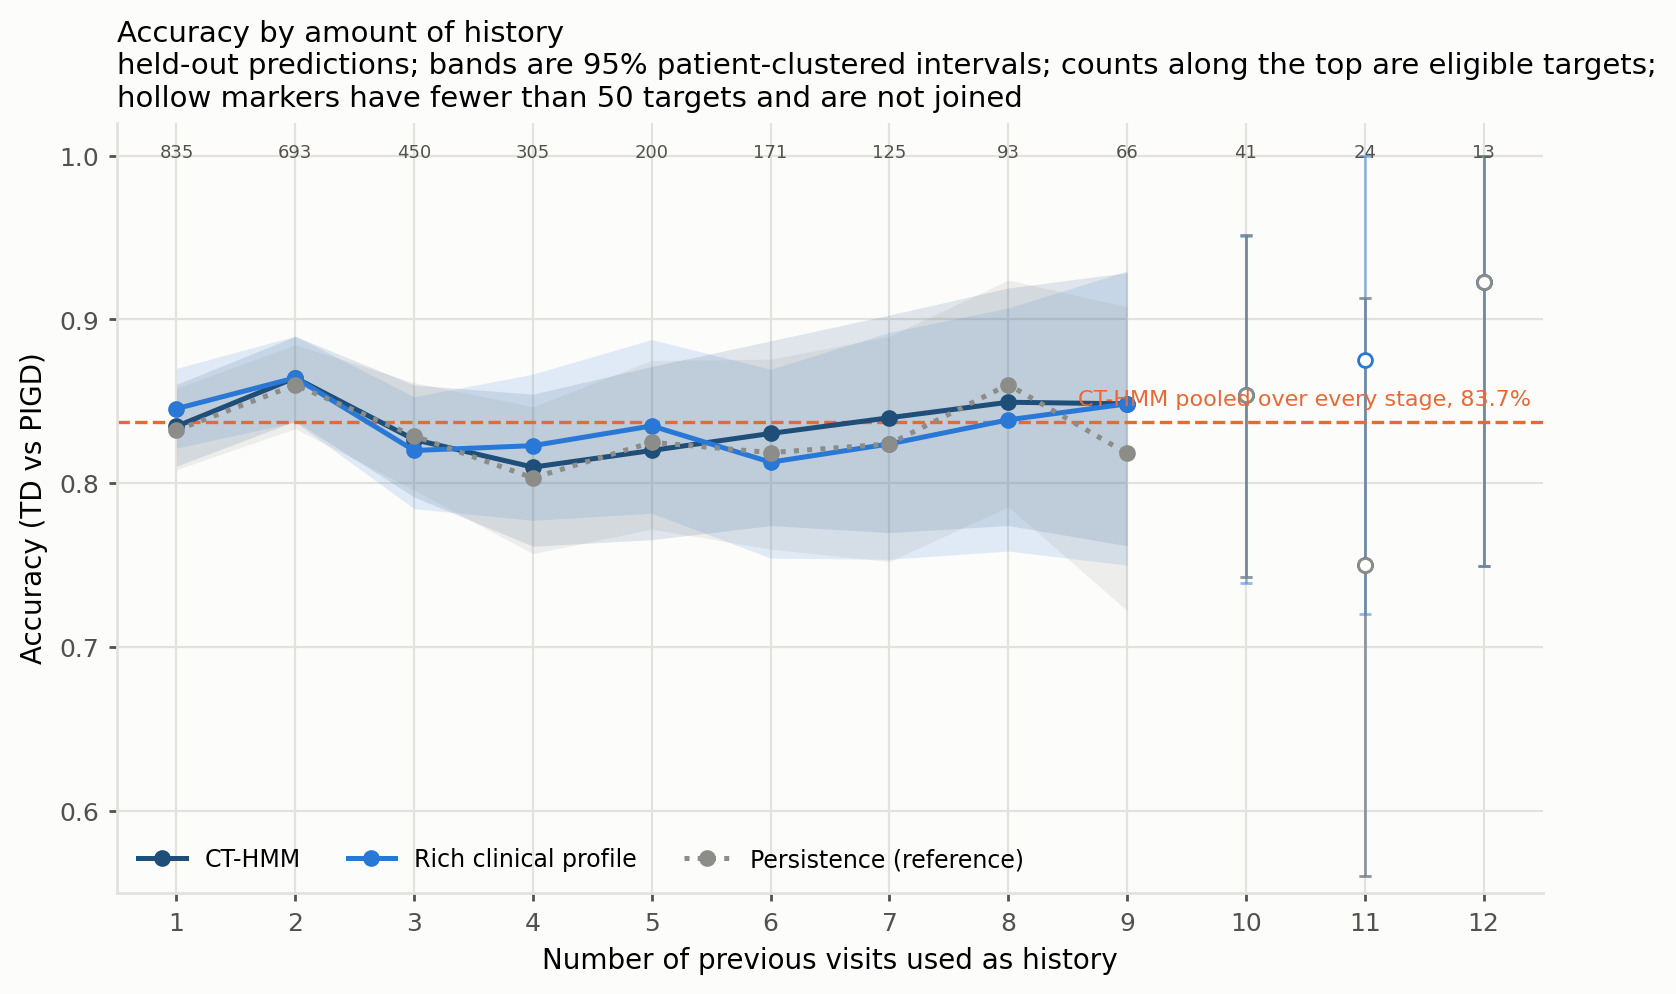
\includegraphics[width=0.80\textwidth]{s07_stage.png}
\caption{Two-class accuracy by prediction stage for the hidden Markov model, the
nine-domain profile and the persistence rule, with patient-clustered bootstrap
intervals. Late stages are small and selected on follow-up.}
\label{sfig:stage}
\end{figure}

\paragraph{Limitation.} Late stages are small and comprise patients selected on
long follow-up.

% --------------------------------------------------------------------
\section{History windows and training regime}
\label{sup:history}
% --------------------------------------------------------------------

Table~\ref{stab:history} collects the four designs that test whether the ceiling
is explained by the amount of history available or by how the model was trained.

\paragraph{Two visits are enough.} Truncating the hidden Markov model's
prediction-time history to the last two visits changes accuracy by $-0.0041$
($-0.0189$ to $+0.0100$) and AUC by $-0.0045$, both intervals containing zero;
three and five visits are likewise indistinguishable from the full record. Only a
single visit is measurably worse, by $-0.0218$ in accuracy and $-0.0617$ in AUC,
because with one visit the model has no run length to read
(Figure~\ref{sfig:windows}). The profile behaves identically.

\paragraph{Retraining on short windows is harmful.} Refitting the model on
two-visit sliding windows costs $-0.0312$ ($-0.0441$ to $-0.0183$) in balanced
accuracy, $-0.0210$ in AUC and $+0.0397$ in log loss against the full-sequence
model. A $2\times2$ design attributes the loss to the change in \emph{training}
($-0.0248$ balanced accuracy with prediction history held fixed) rather than to
the history restriction ($-0.0064$, interval containing zero). The window-trained
model falls \emph{below} persistence in balanced accuracy, through a loss of PIGD
sensitivity (0.608 against 0.706). The fitted parameters show why: the initial
Indeterminate probability falls from 0.155 to 0.044 and the Indeterminate
emission diagonal rises off its floor from 0.500 to 0.665, because a window's
first visit is treated as a draw from the initial distribution and the model
learns to explain every window's start rather than the cohort's baseline
(Figure~\ref{sfig:retrained}). Disjoint windows recover some of the AUC but halve
the training set.

\paragraph{The medication input is not doing hidden work.} Substituting the
current visit's levodopa-equivalent dose for the next visit's changes the
profile's accuracy by $-0.0013$ ($-0.0056$ to $+0.0026$), so knowing the target
visit's prescribed dose is worth nothing.

\begin{table}[htbp]
\centering
\caption{History windows and training regime, for the hidden Markov model and for
the nine-domain profile. All comparisons are paired on common targets.}
\label{stab:history}
\footnotesize
\begin{tabular}{@{}llrll@{}}
\toprule
Model & Comparison & $\Delta$ accuracy & 95\% CI & $\Delta$ AUC (95\% CI) \\
\midrule
\multicolumn{5}{@{}l}{\textit{(a) Truncated prediction history, hidden Markov model (734 common targets, 228 patients)}}\\
HMM & last 2 $-$ full (primary) & $-0.0041$ & ($-0.0189$, $+0.0100$) & $-0.0045$ ($-0.0150$, $+0.0043$) \\
HMM & last 3 $-$ full           & $+0.0027$ & ($-0.0065$, $+0.0117$) & $+0.0014$ ($-0.0032$, $+0.0061$) \\
HMM & last 5 $-$ full           & $+0.0014$ & ($+0.0000$, $+0.0043$) & $+0.0001$ ($-0.0009$, $+0.0011$) \\
HMM & last 1 $-$ full           & $-0.0218$ & ($-0.0423$, $-0.0014$) & $-0.0617$ ($-0.0858$, $-0.0385$) \\
\addlinespace[3pt]
\multicolumn{5}{@{}l}{\textit{(b) Truncated prediction history, rich clinical profile (1,489 common targets, 481 patients)}}\\
Profile & last 2 $-$ full (primary) & $-0.0007$ & ($-0.0102$, $+0.0085$) & $-0.0025$ ($-0.0069$, $+0.0016$) \\
Profile & last 3 $-$ full           & $+0.0020$ & ($-0.0062$, $+0.0096$) & $+0.0000$ ($-0.0030$, $+0.0030$) \\
Profile & current-visit medication substituted & $-0.0013$ & ($-0.0056$, $+0.0026$) & $+0.0003$ ($-0.0008$, $+0.0014$) \\
\addlinespace[3pt]
\multicolumn{5}{@{}l}{\textit{(c) Retraining the hidden Markov model on two-visit windows (2,192 common targets, 742 patients)}}\\
\multicolumn{2}{@{}l}{Window-trained, last 2 $-$ full-trained, full (primary)} & $-0.0082$ & ($-0.0193$, $+0.0026$) & $-0.0210$ ($-0.0301$, $-0.0120$) \\
\multicolumn{2}{@{}l}{\quad training effect, history fixed} & $-0.0064$ & ($-0.0155$, $+0.0027$) & $-0.0127$ ($-0.0197$, $-0.0060$) \\
\multicolumn{2}{@{}l}{\quad history effect, training fixed} & $-0.0018$ & ($-0.0089$, $+0.0054$) & $-0.0084$ ($-0.0144$, $-0.0026$) \\
\multicolumn{5}{@{}l}{Balanced accuracy, primary contrast: $-0.0312$ ($-0.0441$, $-0.0183$); PIGD sensitivity 0.608 vs 0.706.}\\
\addlinespace[3pt]
\multicolumn{5}{@{}l}{\textit{(d) The same two designs for the rich clinical profile}}\\
Profile & last 1 $-$ full history   & $-0.0139$ & ($-0.0221$, $-0.0057$) & $-0.0105$ ($-0.0150$, $-0.0062$) \\
Profile & last 2 $-$ full history   & $+0.0046$ & ($-0.0031$, $+0.0123$) & $-0.0026$ ($-0.0060$, $+0.0008$) \\
\multicolumn{2}{@{}l}{Window-trained $-$ full-trained (profile)} & $-0.0040$ & ($-0.0157$, $+0.0083$) & --- \\
\bottomrule
\end{tabular}

\end{table}

\begin{figure}[htbp]
\centering
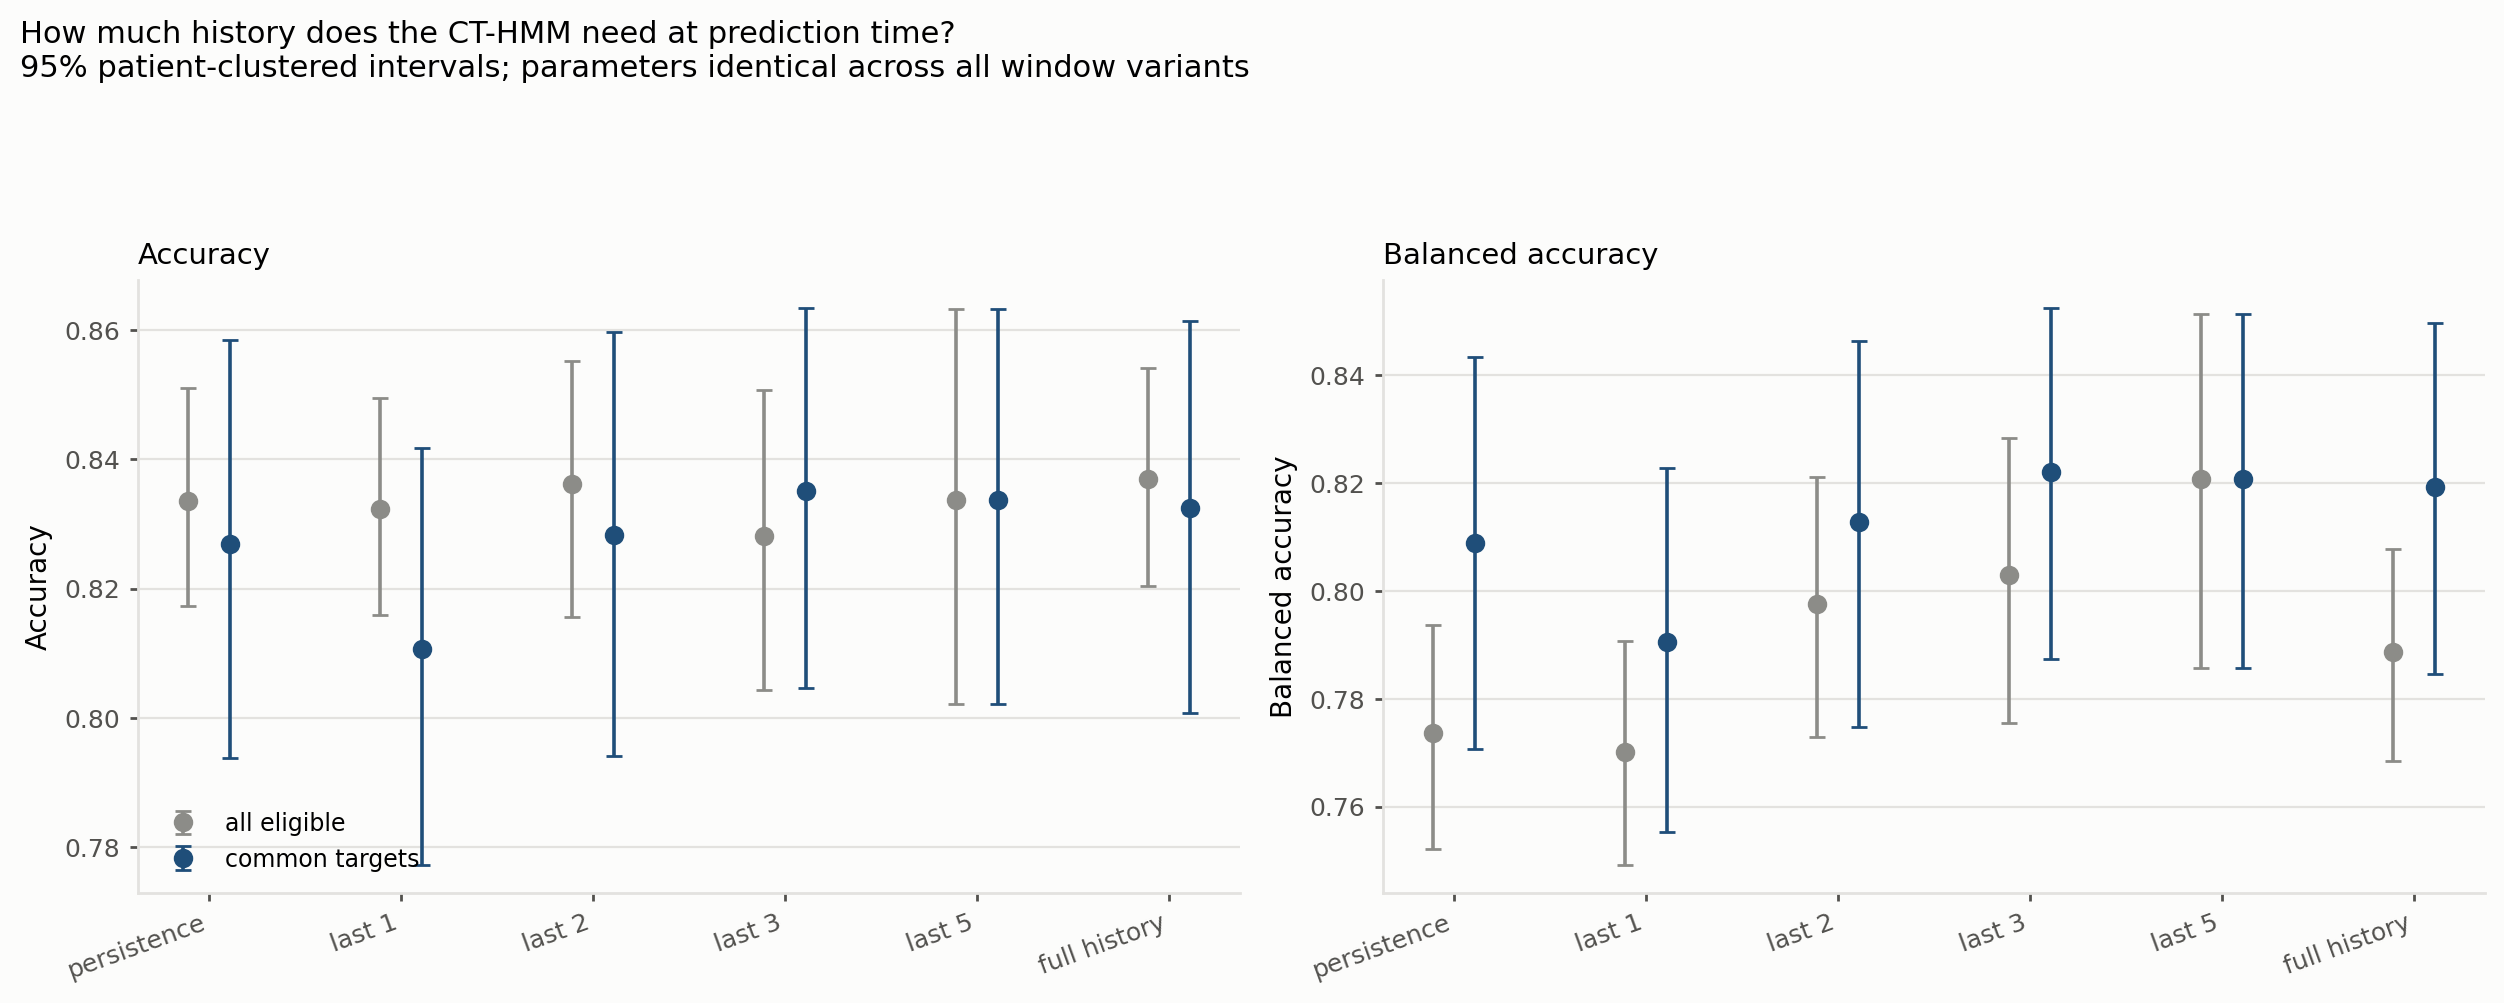
\includegraphics[width=0.80\textwidth]{s08_windows.png}
\caption{Hidden Markov model accuracy by prediction history window, on all
eligible targets and on the common targets every window can score. Only the
single-visit window is measurably worse than the full history.}
\label{sfig:windows}
\end{figure}

\begin{figure}[htbp]
\centering
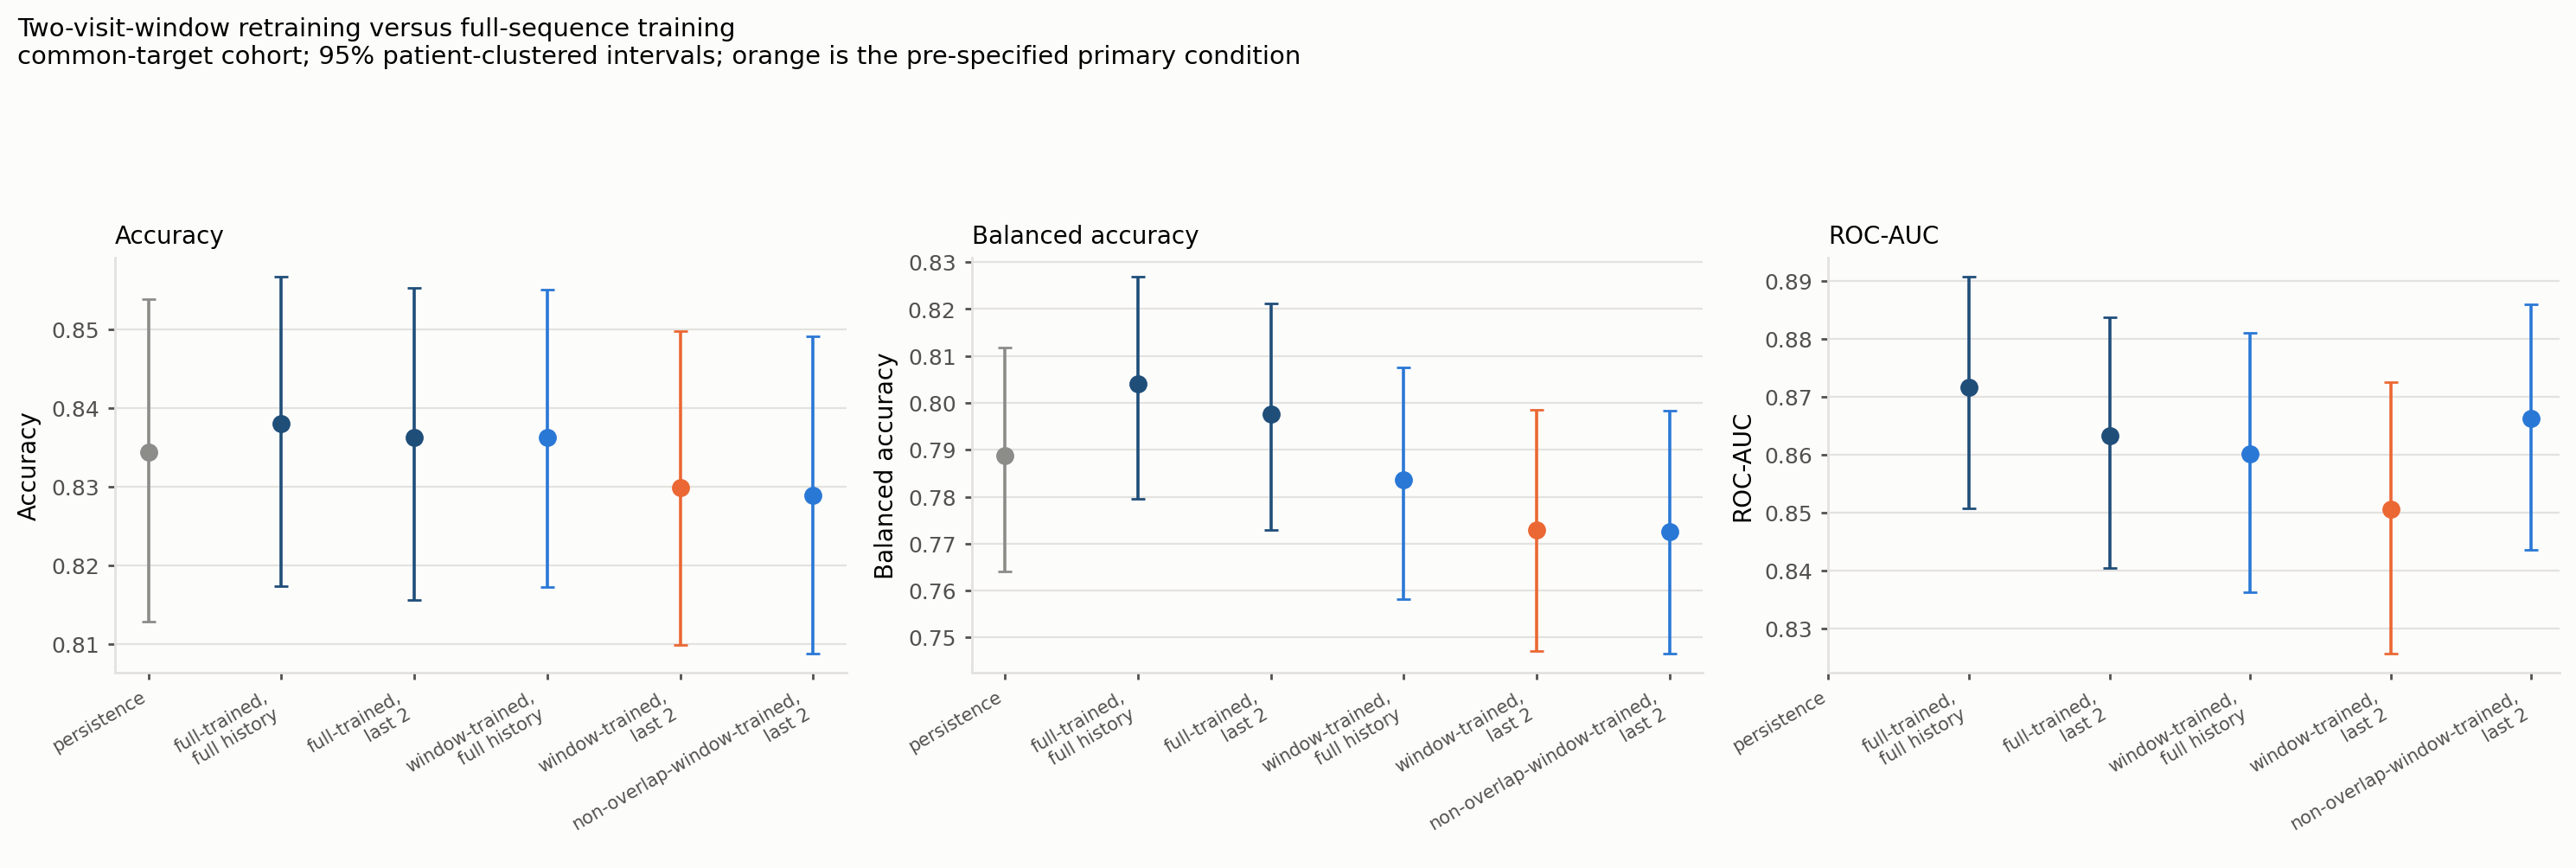
\includegraphics[width=0.84\textwidth]{s09_retrained.png}
\caption{The two-by-two design crossing training regime (full sequences or
two-visit windows) with prediction history (full or last two). The loss is
attributable to the training regime, not to the history restriction.}
\label{sfig:retrained}
\end{figure}

\paragraph{Limitation.} The common cohort for the history-window comparison is the
228 patients with at least six visits, a group selected on long follow-up.

% --------------------------------------------------------------------
\section{Patient-level accuracy}
\label{sup:patient}
% --------------------------------------------------------------------

Visit-level accuracy over-weights patients with long follow-up.
Table~\ref{stab:patient} recomputes every condition at the patient level.

Mean per-patient accuracy is 0.834 (0.817--0.852) against a visit-level 0.839,
but the distribution is bimodal: 63.7\% of patients are predicted correctly at
every eligible visit and 5.0\% at none, with a median of 1.000.

The mode a patient falls in is set by the composition of their recorded target
labels. Patients whose targets are all TD are predicted at 0.944 (persistence
0.970), all PIGD at 0.811 (0.733), majority TD at 0.684 (0.670), majority PIGD at
0.592 (0.541), and evenly split at 0.468 (0.480). \textbf{The persistence rule
shows the same gradient}, so this describes the label sequence rather than model
behaviour.

Per-patient PIGD sensitivity averages 0.550, rising to 0.722 among the 225
patients with at least two PIGD targets, where the share of patients with no
correct PIGD prediction falls from 32.5\% to 6.2\%. TD specificity averages 0.858.

At the patient level the paired comparisons repeat the visit-level ones, with 660
to 828 of the matched patients unchanged under every contrast; the models move at
most a few per cent of patients in either direction relative to persistence.

\begin{table}[htbp]
\centering
\caption{Patient-level accuracy: distribution, composition groups, class-specific
rates and paired comparisons.}
\label{stab:patient}
\small
\begin{tabular}{@{}lrrrrr@{}}
\toprule
\multicolumn{6}{@{}l}{\textit{(a) Distribution of per-patient two-class accuracy}}\\
Condition & $n$ patients & Visit-level & Mean patient & Median & \% perfect \\
\midrule
Profile, full history   & 898 & 0.8391 & 0.8342 & 1.000 & 63.7 \\
Profile, last 2 visits  & 740 & 0.8425 & 0.8395 & 1.000 & 68.2 \\
Profile, last 1 visit   & 898 & 0.8252 & 0.8219 & 1.000 & 63.3 \\
Persistence             & 898 & 0.8338 & 0.8307 & 1.000 & 63.1 \\
\multicolumn{6}{@{}l}{Profile, full history: 5.0\% of patients correct at no visit; 8.2\% below 50\%; 70.9\% at 80\% or better.}\\
\midrule
\multicolumn{6}{@{}l}{\textit{(b) Per-patient accuracy by the composition of that patient's recorded target labels}}\\
Composition & $n$ patients & $n$ targets & Profile & Persistence & \\
\midrule
All TD targets      & 510 & 1,461 & 0.9444 & 0.9697 & \\
Majority TD         & 105 & 600   & 0.6838 & 0.6704 & \\
Evenly split        & 60  & 188   & \textbf{0.4685} & \textbf{0.4799} & \\
Majority PIGD       & 61  & 333   & 0.5921 & 0.5413 & \\
All PIGD targets    & 162 & 439   & 0.8112 & 0.7330 & \\
\midrule
\multicolumn{6}{@{}l}{\textit{(c) Per-patient class-specific rates}}\\
\multicolumn{2}{@{}l}{Mean PIGD sensitivity, all patients with PIGD targets} & \multicolumn{2}{r}{0.5503} & \multicolumn{2}{l}{(persistence 0.4679)} \\
\multicolumn{2}{@{}l}{\quad among patients with $\geq 2$ PIGD targets} & \multicolumn{2}{r}{0.7222} & \multicolumn{2}{l}{(persistence 0.6537)} \\
\multicolumn{2}{@{}l}{Mean TD specificity} & \multicolumn{2}{r}{0.8583} & \multicolumn{2}{l}{(persistence 0.8834)} \\
\midrule
\multicolumn{6}{@{}l}{\textit{(d) Patient-level paired comparisons (mean difference, patients improved / worsened / unchanged)}}\\
\multicolumn{2}{@{}l}{Last 1 vs full history} & $-0.0123$ & \multicolumn{3}{l}{($-0.0225$, $-0.0017$); 46 / 78 / 774} \\
\multicolumn{2}{@{}l}{Last 2 vs full history} & $+0.0080$ & \multicolumn{3}{l}{($-0.0000$, $+0.0164$); 41 / 30 / 669} \\
\multicolumn{2}{@{}l}{Window-trained vs full-trained} & $-0.0040$ & \multicolumn{3}{l}{($-0.0157$, $+0.0083$); 36 / 44 / 660} \\
\multicolumn{2}{@{}l}{Full history vs persistence} & $+0.0029$ & \multicolumn{3}{l}{($-0.0078$, $+0.0141$); 72 / 58 / 768} \\
\bottomrule
\end{tabular}

\end{table}

\paragraph{Limitation.} The composition groups are defined from the outcomes and
are exploratory; nothing about severity or progression can be read from them.

% --------------------------------------------------------------------
\section{The band-width sweep}
\label{sup:bands}
% --------------------------------------------------------------------

Section~\ref{sec:richer} reports that adding the ratio band to the observation
alphabet raises ranking without raising accuracy. This section asks whether the
chosen band width was a poor one. Table~\ref{tab:bands} of the main text gives
the five-width sweep; Figure~\ref{sfig:bandwidth} plots it.

Accuracy lies between 0.832 and 0.836 at every width against 0.837 unbanded, and
every accuracy contrast includes zero. AUC-ROC is 0.874 to 0.878 across widths
against 0.859 unbanded, and every width gains AUC by an interval excluding zero.
Against the reference width of 0.10, width 0.30 is better on all three ranking
metrics by intervals that exclude zero, but the margins are a few thousandths;
against the \emph{unbanded} model, no width gains average precision or partial
AUC, the two ranking metrics that weight the operating region.

The optimum is interior and arises where the alphabet is coarse enough that every
category holds at least eight training observations: at width 0.05 the alphabet
has 73 categories and 28 of them hold fewer than ten observations, against zero
at width 0.50. Brier score, log loss and the calibration gap are all best at width
0.30 and all worse than the unbanded model's.

\paragraph{Conclusion.} The reference width was not a poor choice, the optimum is
not worth having, and \textbf{no width turns the ranking gain into an accuracy or
calibration gain}. The conclusion of the main text is insensitive to the band
width.

\begin{figure}[htbp]
\centering
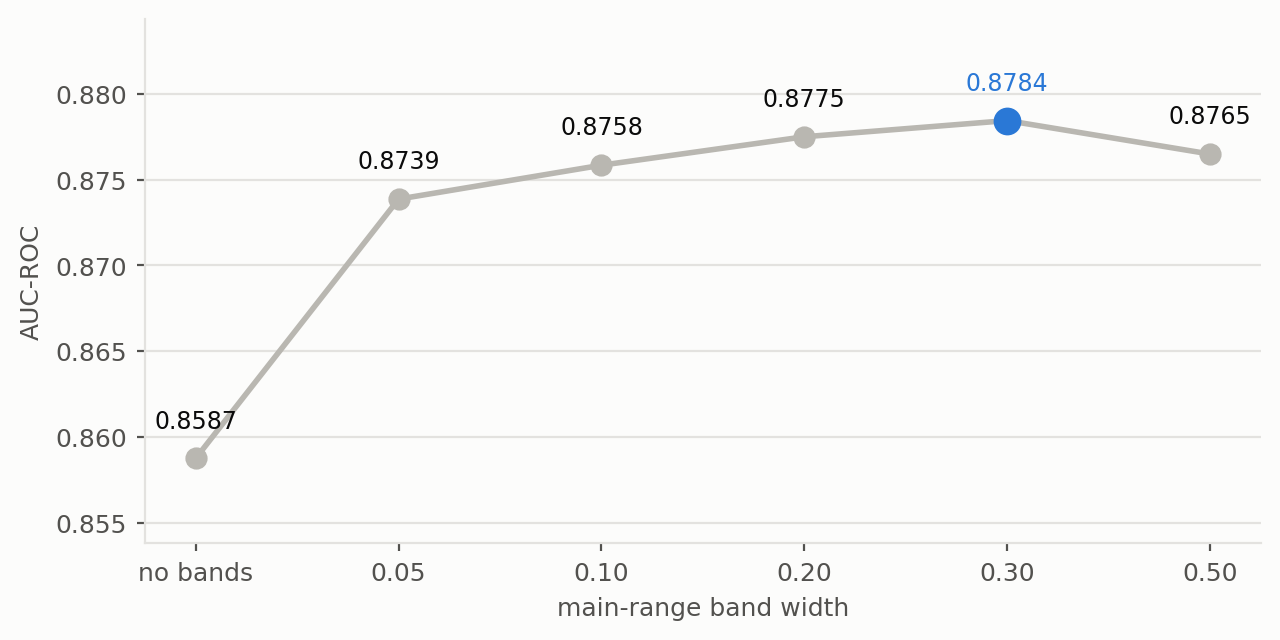
\includegraphics[width=\textwidth]{s10_bandwidth.png}
\caption{Band-width sweep: area under the ROC curve by main-range band width,
against the unbanded model at the left. Every banded width gains AUC over the
unbanded model, and the interior optimum near 0.30 (highlighted) is worth a few
thousandths of AUC over the rest. Average precision and partial AUC are in
Table~\ref{tab:bands} of the main text and do not share this optimum.}
\label{sfig:bandwidth}
\end{figure}

\paragraph{Limitations.} Five widths; the tail structure is common to all arms;
the sweep is a sensitivity analysis and was not pre-registered as a selection.

% --------------------------------------------------------------------
\section{Complete analysis inventory}
\label{sup:inventory}
% --------------------------------------------------------------------

Table~\ref{stab:inventory} lists every analysis in the programme that bears on the
question of this paper, with its cohort, its status and where it is reported. The
table is the completeness record for the study: every completed analysis appears
either in the main text or in this supplement, and the two analyses that were
specified but never run on the cohort are listed as such and described in
\ref{sup:notrun}.

Analyses belonging to a separate line of work on unsupervised structure in the
cohort are outside the scope of this paper, contribute to none of its results,
and are not listed.

\begin{small}
\begin{longtable}{@{}p{0.40\textwidth}p{0.27\textwidth}p{0.11\textwidth}p{0.14\textwidth}@{}}
\toprule
Analysis & Cohort / units & Status & Reported in \\
\midrule
\endfirsthead
\toprule
Analysis & Cohort / units & Status & Reported in \\
\midrule
\endhead
\multicolumn{4}{@{}l}{\textit{The target: how the label is built and how fragile it is}}\\
Cohort construction and participant flow & 1,080 pt / 5,774 visits & completed & \S\ref{sec:data} \\
Exact reconstruction of the label from raw items & 1,080 pt / 5,774 visits & completed & \S\ref{sec:construction} \\
Label agreement between OFF and ON examinations & 714 pt / 2,343 pairs & completed & \S\ref{sec:construction} \\
Attainable ratios on the integer lattice & 4,441 labelled visits & completed & \S\ref{sec:construction} \\
Threshold-placement sensitivity & 1,080 pt / 4,441 visits & completed & \S\ref{sec:construction} \\
\addlinespace[3pt]
\multicolumn{4}{@{}l}{\textit{The dynamics of the label, measured before any model}}\\
Transition structure, reversion, conversion, interval dependence & 934 pt / 3,361 transitions & completed & \S\ref{sec:dynamics} \\
First-order Markov property in the recorded label & 2,427 triples & completed & \S\ref{sec:dynamics} \\
Pre-registered audit of the Indeterminate class & 934 pt & completed; inconclusive by its own rule & \S\ref{sec:dynamics}, \ref{sup:ind} \\
Lag-1 autocorrelation of within-patient residual change & 397 pt / 2,050 pairs & completed & \S\ref{sec:dynamics} \\
\addlinespace[3pt]
\multicolumn{4}{@{}l}{\textit{Can a generative model of the ratio reproduce the label?}}\\
Pre-registered posterior-predictive label check & 821 pt / 3,528 visits & completed; negative & \S\ref{sec:ppc} \\
Diagnostic localisation of the misfit & 821 pt / 3,528 visits & completed; descriptive & \S\ref{sec:ppc}, \ref{sup:ppc} \\
\addlinespace[3pt]
\multicolumn{4}{@{}l}{\textit{Models of the label itself}}\\
Chains and the latent-state model on one split & 1,002 held-out pairs & completed & \ref{sup:hmm} \\
Leave-one-patient-out three-class prediction & 934 pt / 3,361 transitions & completed & \S\ref{sec:discrete} \\
Uniqueness of the fitted optimum; configuration sensitivity & 934 pt / 3,361 & completed & \ref{sup:hmm} \\
Five latent states & 934 pt / 3,361 & completed; negative, 404/934 folds converged & \S\ref{sec:discrete}, \ref{sup:hmm} \\
Prediction with no history (first-visit model) & 1,002 held-out rows & completed & \ref{sup:firstvisit} \\
\addlinespace[3pt]
\multicolumn{4}{@{}l}{\textit{Models of the continuous quantity the label is cut from}}\\
Hierarchical Bayesian growth model of the ratio & 821 pt; 825 matched pairs & completed & \S\ref{sec:continuous} \\
Student-t slope and residual variants & 821 pt / 7 splits & completed & \ref{sup:studentt} \\
Gaussian-process regression of the ratio & 821 pt / 2,707 points & completed & \S\ref{sec:continuous} \\
Independent Gaussian processes on the two subscores & 934 pt / 3,361 points & completed & \S\ref{sec:continuous} \\
Joint bivariate mixed model of the subscores & 934 pt / 8,590 obs & completed & \ref{sup:subscore} \\
Multi-output Gaussian processes & 934 pt / 3,361 points & completed & \ref{sup:subscore} \\
Fifteen-arm held-out subscore comparison & 934 pt / 3,361 points & completed & \ref{sup:subscore} \\
Time-varying spline model of the subscore rates & 934 pt & completed & \ref{sup:temporal} \\
Identifiability and interval audit of that model & 934 pt & completed & \ref{sup:temporal} \\
\addlinespace[3pt]
\multicolumn{4}{@{}l}{\textit{The harmonised comparison}}\\
Fourteen specifications under one decision rule & 934 pt / 3,361 transitions & completed & \S\ref{sec:harmonised} \\
Decomposition of each margin by current label & 934 pt / 3,361 transitions & completed & \S\ref{sec:harmonised} \\
\addlinespace[3pt]
\multicolumn{4}{@{}l}{\textit{Does a richer observation help?}}\\
Two-class next-visit prediction, seven models & 899 pt / 3,029 transitions & completed & \S\ref{sec:richer} \\
Discrete latent state over ten clinical measurements & 654 pt / 2,091 cases & completed; negative & \S\ref{sec:richer}, \ref{sup:clinical} \\
Continuous level-and-rate profile over nine domains & 934 pt / 3,353 predictions & completed & \S\ref{sec:richer} \\
Profile-derived label against the latent-state model & 898 pt / 3,020 transitions & completed & \S\ref{sec:richer} \\
Information criteria within likelihood families & full cohort & completed & \ref{sup:misc} \\
Threshold-free discrimination of next-visit PIGD & 898 pt / 3,020 transitions & completed & \S\ref{sec:richer} \\
Ratio band added to the observation alphabet & 899 pt / 3,029 transitions & completed & \S\ref{sec:richer} \\
Band-width sweep over five widths & 899 pt / 3,029 transitions & completed & \S\ref{sec:richer}, \ref{sup:bands} \\
\addlinespace[3pt]
\multicolumn{4}{@{}l}{\textit{Where and when prediction fails}}\\
Model calls at Indeterminate visits & 220 pt / 287 visits & completed & \ref{sup:misc} \\
Accuracy by prediction stage & 896 pt / 3,017 targets & completed & \ref{sup:stage} \\
Truncated prediction history, latent-state model & 228 pt / 734 common targets & completed & \S\ref{sec:ceiling}, \ref{sup:history} \\
Truncated prediction history, clinical profile & 481 pt / 1,489 common targets & completed & \ref{sup:history} \\
Retraining the latent-state model on two-visit windows & 742 pt / 2,192 targets & completed; negative & \ref{sup:history} \\
Truncated history and retraining for the profile & 898 / 740 pt & completed & \ref{sup:history} \\
Patient-level distribution of accuracy & 898 pt & completed & \S\ref{sec:ceiling}, \ref{sup:patient} \\
\addlinespace[3pt]
\multicolumn{4}{@{}l}{\textit{Specified but not run on the cohort}}\\
Integer-score measurement model of the items & --- & synthetic recovery only; not run on real data & \ref{sup:notrun} \\
Re-execution saving per-visit replicate labels & --- & specified, reviewed, not run & \ref{sup:notrun} \\
\bottomrule
\end{longtable}

\end{small}
\label{stab:inventory}

% --------------------------------------------------------------------
\section{Work specified but not run}
\label{sup:notrun}
% --------------------------------------------------------------------

Two analyses were specified in full, implemented, and tested on synthetic data,
but never run on the cohort. Neither supports any result in this paper, and
neither is reported as a finding. They are recorded here because the first is the
analysis the posterior-predictive diagnostics of Section~\ref{sec:ppc} identified
as the decisive next test.

\paragraph{An integer-score measurement model of the items.} The diagnostics in
\ref{sup:ppc} attribute the generative model's failure to the integer lattice
rather than to an additional state. The implied test is a model of the item scores
themselves --- an ordinal item-response specification with adaptive
Gauss--Hermite quadrature, carrying no intermediate state --- asking whether a
measurement-faithful generator reproduces the Indeterminate share without one.
The specification passed its synthetic parameter-recovery tests. It was never run
on the cohort, so \textbf{whether such a model reproduces the label record is
unresolved}, and this paper draws no conclusion about it.

\paragraph{A re-execution saving per-visit replicate labels.} The
posterior-predictive check did not retain the per-visit replicate labels, which is
why the diagnostics in \ref{sup:ppc} are referenced to a covariate-blind
generator rather than to the patient-conditional replicate distribution the check
itself used. A protocol-compliant re-execution that would have saved them was
specified and reviewed but not run. This limits the diagnostics to a descriptive
localisation of the misfit; it does not affect the check's verdict, which is based
on the saved omnibus statistic and its pre-registered threshold.


\end{document}
